\chapter{Temporary Muon Spectrometer}
\label{ch:tms}



%%%%%%%%%%%%%%%%%%%%%%%%%%%%%%%%
\section{Overview of the \dshort{tms}}
\label{sec:tms-ovvw}

%%%%%%%%%%%%%%%
\subsection{Introduction and Scope}
\label{sec:tms-ovvw-intro}

The \dword{dune} Collaboration's goal is to have a gaseous argon \dword{tpc} (\dword{ndgar}) in a magnetic field immediately downstream of a liquid argon \dword{tpc}(\dword{ndlar}), to measure the momenta of muons exiting the liquid, as well as to study neutrino-argon interactions in more detail. This is foreseen to be primarily a non-US contribution, and is presently not on a timescale guaranteed to be ready when \dword{dune} operations to begin. The \dword{tms} is therefore intended to operate for the early part of the running when beam intensities are at their lowest and \dword{dune} is not systematics limited.

This instrument is designed to have very low technical risk, be inexpensive, and have a well-understood construction time, to allow maximum flexibility to take advantage of positive developments on the international front. To that end, we intend to advance a mechanical design to the point where the go/no-go decision date is well-understood, but to defer the full electronics design until we are closer to that point, lest we do a detailed design around components that will have become obsolete.

%%%%%%%%%%%%%%%Not in Tim's new organization
\subsection{Design and Principle of Operation}
\label{sec:tms-ovvw-op}

The \dword{tms} is a magnetized steel range stack between \dword{ndlar} and \dword{sand}. The purpose of the Muon Spectrometer is to measure the charge and momentum of muons that exit \dword{ndlar} with a momentum precision comparable to the Far Detector (taken to be 4\%) in the kinematically relevant region of  \SIrange{1}{5}{\GeV}.  The face is the same size as \dword{ndlar} and the depth in the beam direction is \SI{7}{\m}.  It consists of four columns of scintillator modules and three columns of steel; each row is \num{100} layers, with each layer containing \num{192} scintillator strips in modules of \num{48}. Panels are tilted $\pm 3^{\circ}$ in alternating U and V views. The detector is shown in Figure \ref{fig:tms_anl_fig1}. 

\begin{dunefigure}[The \dword{tms} support structure, steel plates, modules and coils]{fig:tms_anl_fig1}
{The \dword{tms} support structure, upstream \SI{15}{\mm} steel plates (green), downstream \SI{40}{\mm} steel plates (blue), modules (grey), and coils (orange).  Current in the two central coils flows in the opposite direction as the left-most and right-most coils, producing magnetic fields that are upward in the left and right-most steel columns, and down in the central steel column.}
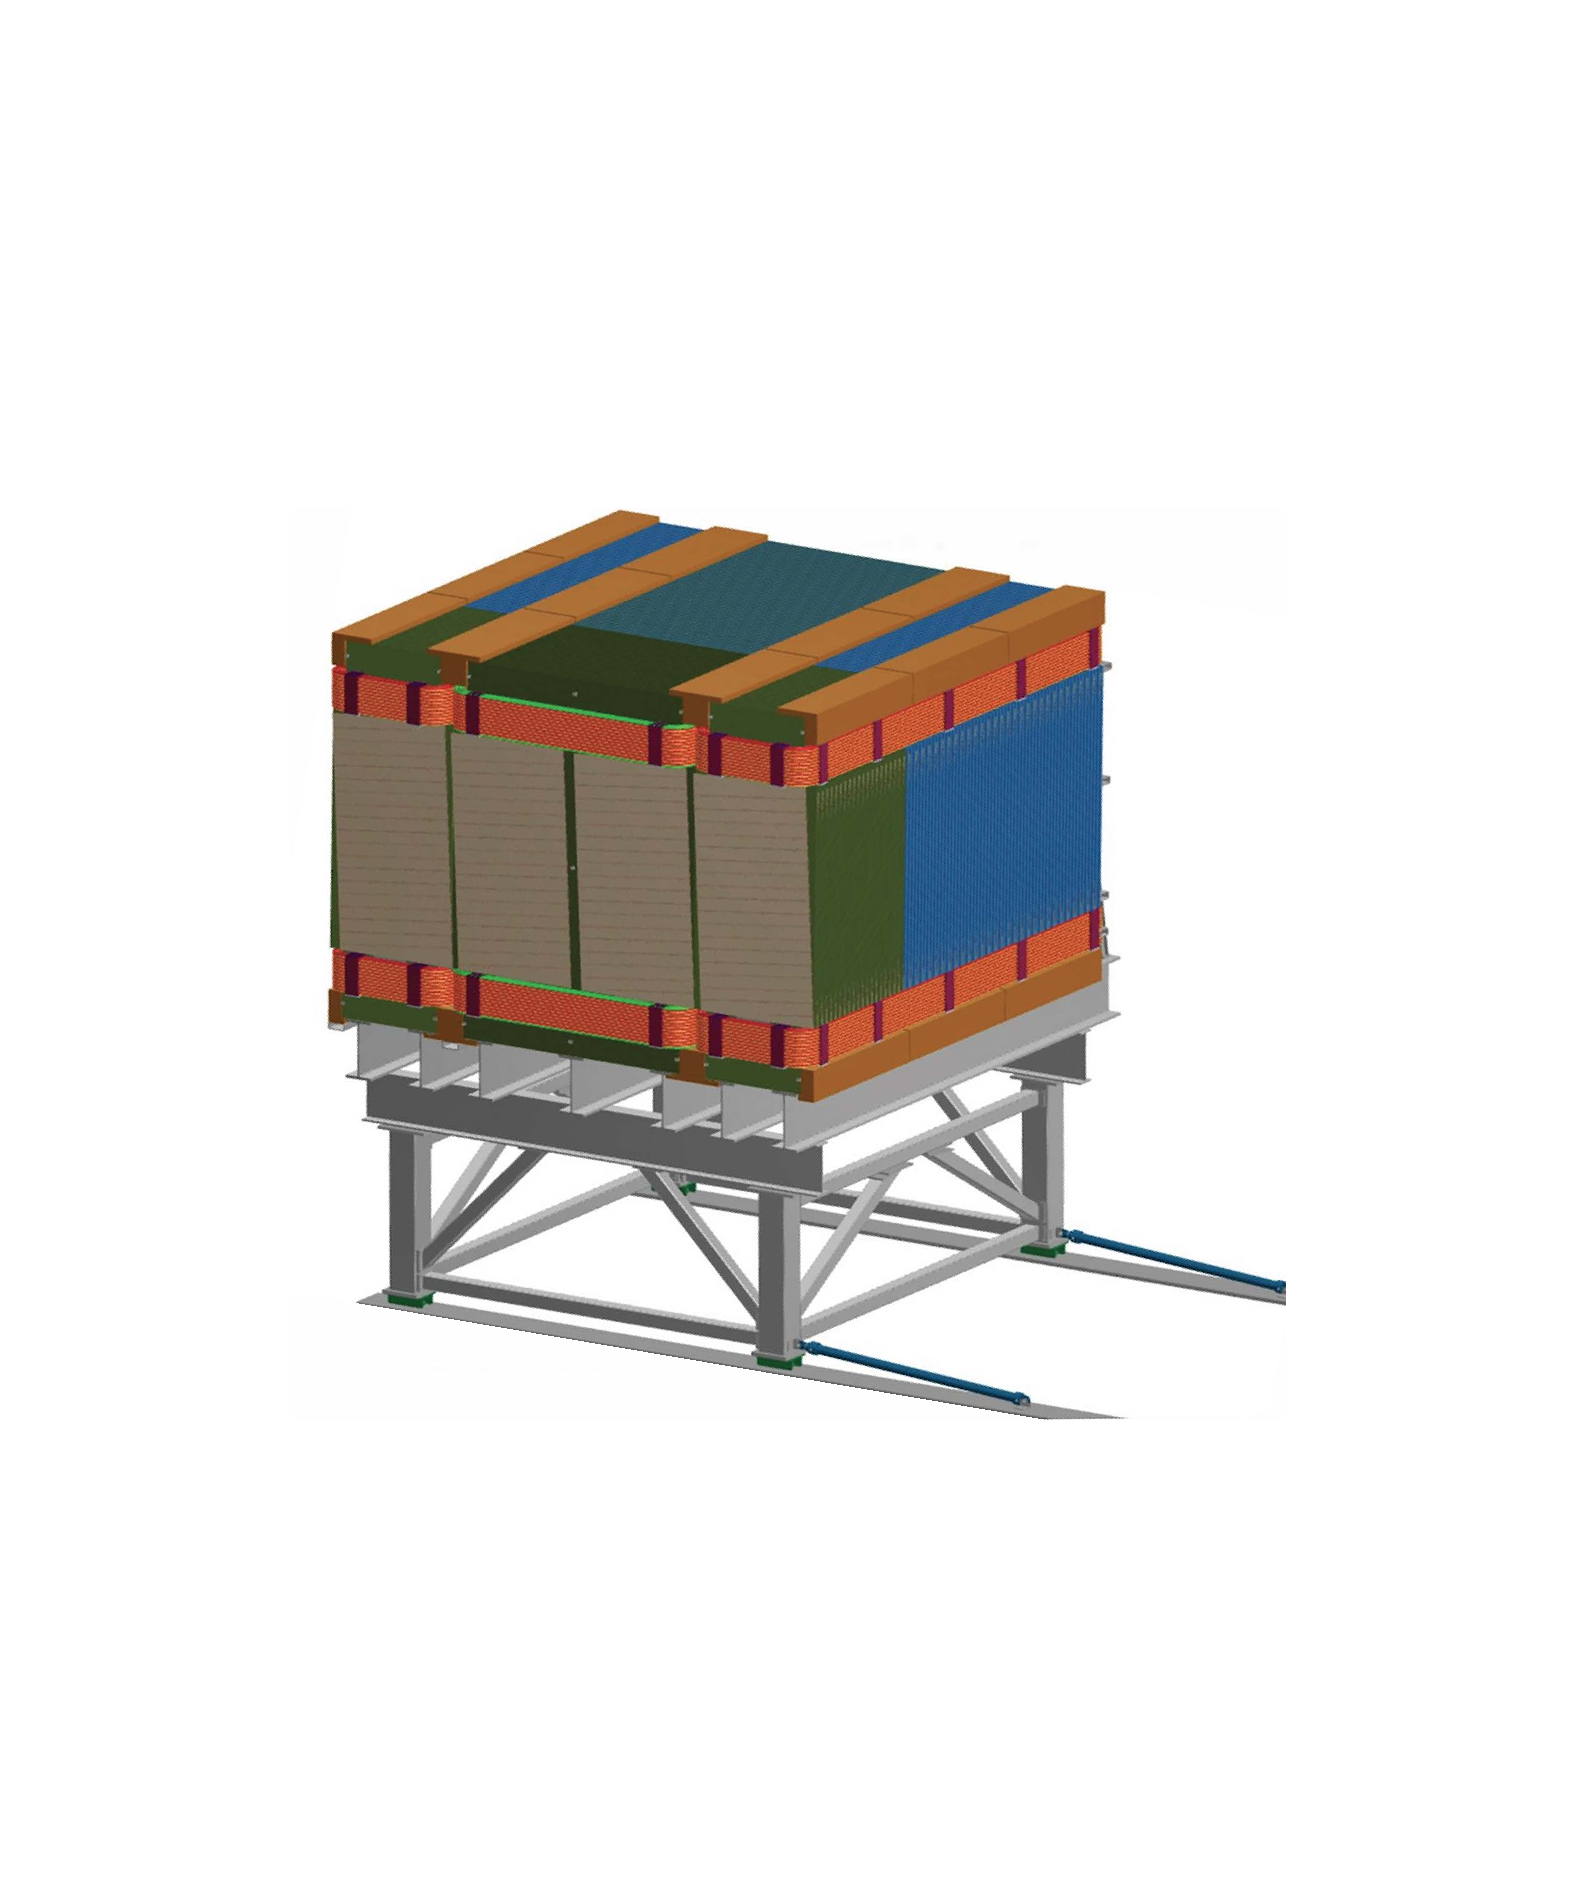
\includegraphics[width=0.55\textwidth]{graphics/tms/Detector/tms_anl_iso2.pdf}
\end{dunefigure}

The device measures muon energy by measuring the range, not via magnetic bend. At muon energies in the relevant range for this detector, $E < 5$~GeV, the range is expected to be the best estimator of energy. This sets the number of layers, as the ability to measure range is equivalent to measuring the last layer the muon traverses. Measuring to a resolution of 4\% implies that adjacent layers should be spaced about 4\% apart, but this would lead to \num{100} different plate thicknesses. We approximate this by having two widths: the upstream \num{40} layers are 15~mm thick, driven by manufacturability concerns, and the downstream \num{60} layers are 40~mm thick, to maximize the threshold energy for muons to stop. More details are shown in Section \ref{sec:muonres}).

The energy in each counter is recorded using a 12-bit ADC. Measuring muon energy via calorimetry is not competitive with range, as we would expect a resolution of $(15-20\%)/\sqrt{E}$, but it provides four benefits:
\begin{itemize}
\item{Muons that have undergone exceptionally high energy loss, for instance from a large energy bremsstrahlung can be potentially identified and either be removed from analysis or have a correction applied. This could reduce tails from the resolution.}
\item{Muons nearing their stopping point increase their ionization by a factor $1/\beta^2$. Fitting this can improve resolution on the exact stopping point. } 
\item{Muons stopping in the scintillator itself will show a Bragg peak. } 
\item{The signal has a weak dependence on the muon's $y$-position. } 
\end{itemize}

None of these would be sufficient to devote substantial resources to energy measurement, but electronics cost is such that the cost impact is minimal: integrated front-end chips with 12-bit ADCs are available at comparable costs to ones that have only a single bit latch.

The purpose of the magnet is charge identification, not momentum measurement. The width of the scintillator is as large as it can be and still separate positive and negative tracks. Charge is determined by fitting hits to both $\mu^+$ and $\mu^-$ hypotheses, and based on fit quality, assigning charge as ``positive'', ``negative'', or ``undetermined'', in the case that both fits are poor. These fits can be either standalone or include tracks in the liquid argon. The charge separation is worst at low energy, because the number of hits in the TMS is small, as is the liquid argon track, as we only can measure soft muons produced near the downstream edge of the liquid argon. 

The scintillator panel design emphasizes precision in the magnet bend view (the $x$-direction). The detectors are arranged in alternating $u$ and $v$ layers, set at $\pm 3 \degree$ from vertical. This provides approximately 45~cm resolution in the non-bend view. Replacing a fraction of the panels with dedicated $y$-direction panels, but this would degrade charge identification, especially at low momentum.

\subsection{Design Parameters}
\label{sec:tms-ovvw-param}

The \dword{dune} \dword{nd} is designed to meet the physics requirements of the \dword{dune} experiment. The eventual statistical uncertainty on the \dword{fd} $\nu_{e}$ rate is less than 3\%, placing stringent requirements on the systematic constraints provided by the \dword{nd}. However, in the early data taking period, the statistical uncertainty in the \dword{fd} dominates and reduces these requirements. As such, the physics goals of the first few years of the \dword{dune} program place less stringent requirements on the \dword{nd}. The \dword{tms} is designed to meet the physics requirements of the initial data taking period of approximately 100 kt-MW-yrs. 
In this period, split equally between horn polarities, 412 (188) oscillated $\nu_{e}$ are expected in \dword{fhc} mode and 84 (176) oscillated $\bar{\nu}_{e}$ in \dword{rhc} mode in the normal (inverted) hierarchy for $\delta_{CP} = 0$,. Thus, the statistical uncertainty on the appearance rate will be $\sim 5-11\%$. Total systematic effects at the level of a few percent, while critical in the long term, do not impact these initial data.

Initial \dword{dune} analyses will use neutrino interactions in the \dword{ndlar} detector to predict the \dword{fd} reconstructed event spectra. The reconstruction precision of the \dword{ndlar} events must be comparable to the \dword{fd}. Most \dword{fd} muons are identified and their momenta measured by range, with a resolution of 4\% 
%and $4\pi$ angular acceptance
. This drives the requirements of the \dword{tms}, which must match this momentum resolution with acceptance that covers the neutrino interaction phase space.
Since the angular acceptance of the \dword{tms} is larger than that of the \dword{ndgar} the acceptance of the \dword{tms} alone is not a limiting factor in the overall performance of the \dword{nd}.

The principal design parameters are given in Table~\ref{tab:table-tms-params}.

\begin{dunetable}
[\dword{tms} Parameters]
{cc}
{tab:table-tms-params}
{Temporary Muon Spectrometer Parameters}
Parameter & Value \\ \toprowrule
Steel dimensions & 7.4 $\times$ 5.0 $\times$ 7.0~m  \\ \colhline
Steel plate thickness & 40 planes of 15~mm, 60 planes of 40~mm  \\ \colhline
Steel mass & 850 tons \\ \colhline
Magnetic Field & Typically 1.0-1.1 Tesla \\ \colhline
Active Area & 20.22 $\rm m^2$ \\ \colhline
Number of detector planes & 100 \\ \colhline
Channels per plane & 192, in 4 panels of 48 each \\ \colhline
Total channels & 19200 \\ \colhline
Timing resolution & $\leq$~19~ns (single RF bucket) \\
% no \colhline on final row
\end{dunetable}

The steel is magnetized to enable identification of muon charge
with better than 98\% accuracy. A particular challenge is that the generated magnetic field needs to be low inside the liquid argon to match the performance of the un-magnetized far detector. The fast timing allows us to resolve which RF bucket produced the muon of interest, which substantially reduces occupancy: fewer than 10\% of RF buckets contain a muon from a neutrino interaction in the liquid argon. Neutrinos will interact in the \dword{tms} steel, but the mean number of such interactions is only about 0.5, most of which will be meters away from the muon of interest.

%%%%%%%%%%%%%%%Not in Tim's new organization - probably belongs elsewhere
\subsection{Performance}
\label{sec:tms-ovvw-perf}
\subsubsection{Discussion of MINOS performance}
%\fixme{Mat will find people to write}
%\fixme{Clarence has some of the MINOS docDB documents if needed}

Perhaps the most similar functional detector to the \dword{tms} is the \dword{minos} near detector, which is a steel-scintillator sampling calorimeter comprised of alternating planes of 2.54 cm thick magnetized (1.28 T) steel and 1 cm thick by 4 cm wide polystyrene scintillator strips \cite{minosNIM}. This detector recently served as the muon spectrometer for particles exiting the \dword{minerva} detector \cite{MINERvA:2006aa}. Figure \ref{fig:minos_resolution} shows the fractional bias for the range based momentum reconstruction of 3-4 GeV muons in \dword{minos} \cite{bhattacharyaMINOS}. A resolution of ~5\% is demonstrated. Some notable difference with the \dword{tms} design are: the beam energy is higher, the magnetic field is toroidal, and the steel is thicker/sampling fraction lower. Nevertheless, this comparison demonstrates the performance that can be expected from this choice of technology. The remainder of this section focuses on the performance studies that are underway to demonstrate that the \dword{tms} design achieves the required performance, however the success of a previous experiment with this technology provides a demonstration of achievable results.   

\begin{dunefigure}[Momentum resolution of the \dword{minos} near detector]{fig:minos_resolution}
{Left: Resolution of momentum measured from range for tracks that stop in the MINOS detector with a true muon energy of 3-4 GeV. The red line shows results of a Gaussian fit performed
between points at half maximum. Right: The log version of the same plot \cite{bhattacharyaMINOS}.
}
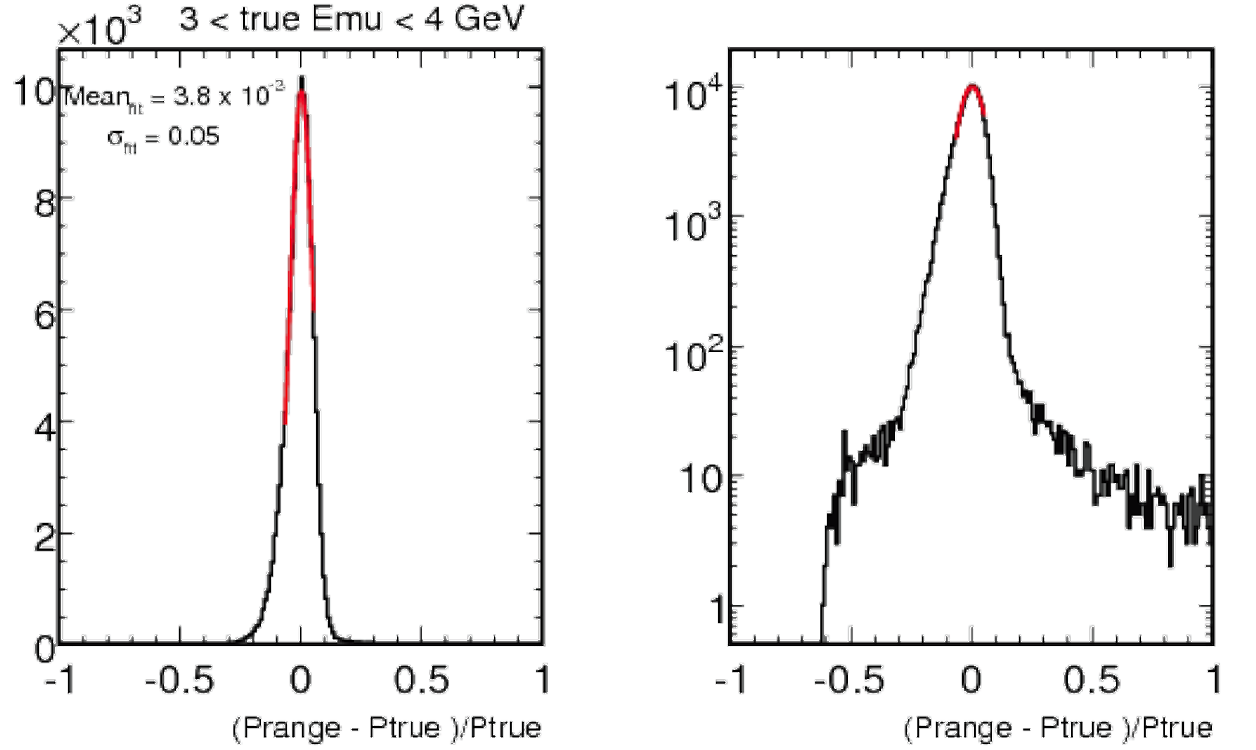
\includegraphics[width=0.7\textwidth]{graphics/tms/Minos/MINOS Resolution.png}
\end{dunefigure}

\subsubsection{Software --- Simulation and Analysis}

Neutrino interactions are simulated with \dword{genie} version 2.12.10 using the physics list \texttt{DefaultPlusValenciaMEC} \cite{Andreopoulos:2009rq}. Particles exiting the struck nucleus are propagated through the \dword{ndlar} and \dword{tms} detectors using a Geant4-based model (edep-sim) \cite{edepsim}.


For most analyses, the signal process is a $\nu_{\mu}$ charged-current interaction in the \dword{ndlar} fiducial volume. The outgoing muon exits the \dword{ndlar} active volume, passes through the cryostat material, and enters the \dword{tms}. Truth level energy deposits in the active scintillator are recorded and used to reconstruct events. 

The analyses presented herein use 10M events generated in the \dword{ndlar} volume from the standard simulated \dword{dune} \dword{fhc} flux . This results in approximately 4M events with energy deposits in the \dword{tms}, and 2M events that are fully contained in the \dword{tms}. 

\subsubsection{Geometry Implementation (GDML)}
A simple Geometry Description Markup Language (GDML) version of the \dword{tms} was created using DUNEggd, an interface to for designing DUNE geometries with the General Geometry Description (GGD) software system \cite{ref:ggd}. This system was chosen to assure compatibility with existing Near Detector geometries of the ND Hall, \dword{ndlar}, GAr, and SAND detectors. 

The geometry consist of 200 total layers of alternating steel (7.85 g/cc, 99\% iron, 0.45\% Si, 0.4\% C by mass) and scintillator (1.05 g/cc, 92\% C, 8\% H by mass). The steel is implemented as 3 plates. The central plate is 3.5 m wide by 3.2 m tall. Plates placed to either side of the central plate measure 1.75 m by 3.2 m. A 2 cm gap separates the side plates from the central plate. The first 40 layers of steel are 1.5 cm thick. The rear 60 layers of steel are 4 cm thick. There is a 4 cm gap between each steel layer. 

The scintillator is implemented as a collection of 3.5~cm wide by 3~m tall by 1~cm thick vertical bars arranged into 1.68 m wide modules. Four modules are placed side by side with a 7 cm gap between the central modules and 9 cm gaps separating inner and outer modules. These scintillator layers are replicated in the gap between steel layers.  

The steel plates are magnetized in the geometry. The thin (thick) central steel plates are given a vertically oriented downward pointing magnetic field of 1.25 T (0.9 T), while the outer steel thin (thick) steel plates have their field pointing upwards with a strength of 1.5 T (1.0 T). This is an older geometry than the one references in Table ~\ref{tab:table-tms-params}. The magnet coils are not currently included, but are expected to sit above and below the scintillator, so we don't expect this to have a major effect. 

This GDML geometry for the \dword{tms} is placed in an existing model of the ND Hall with an existing model of the \dword{ndlar}. The coordinate system for this geometry is defined with $y$ anti-aligned with gravity, $z$ running horizontally in the direction of the beam, and $x$ aligned horizontally to the left of the beam direction. The origin is located at the center point on the hall wall where the beam enters. The \dword{tms} is placed 8.2 m downstream from the \dword{ndlar} (center to center) and centered 2.51 m below the origin in y.   

Figures \ref{fig:geom_in_hall} and \ref{fig:geom_3d} show the geometry.

%\begin{dunefigure}[]{fig:geom_front}
%{Upstream view of the TMS geometry in black and \dword{ndlar} in %yellow.}
%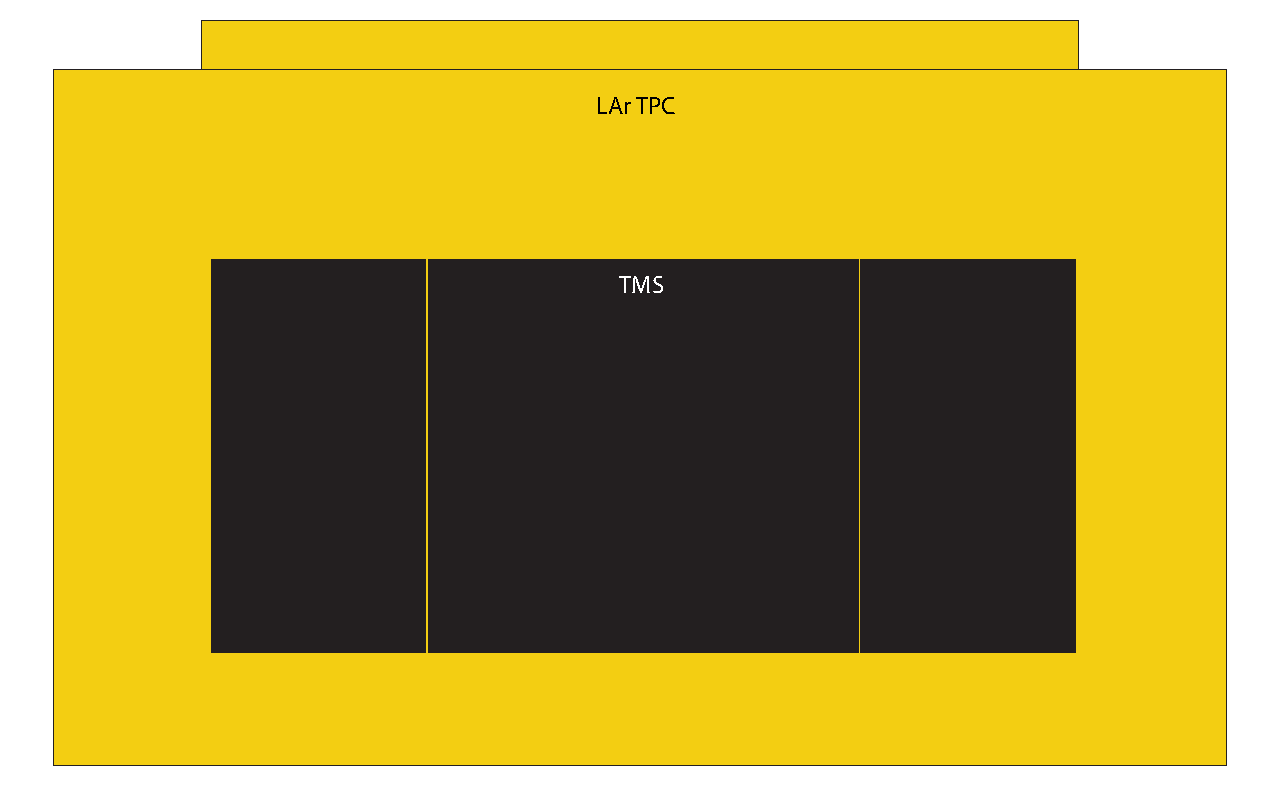
\includegraphics[width=0.8\textwidth]{graphics/tms/Geometry/front_view.pdf}
%\end{dunefigure}
%\begin{dunefigure}[]{fig:geom_top}
%{Top view of the TMS geometry in black and \dword{ndlar} in yellow.}
%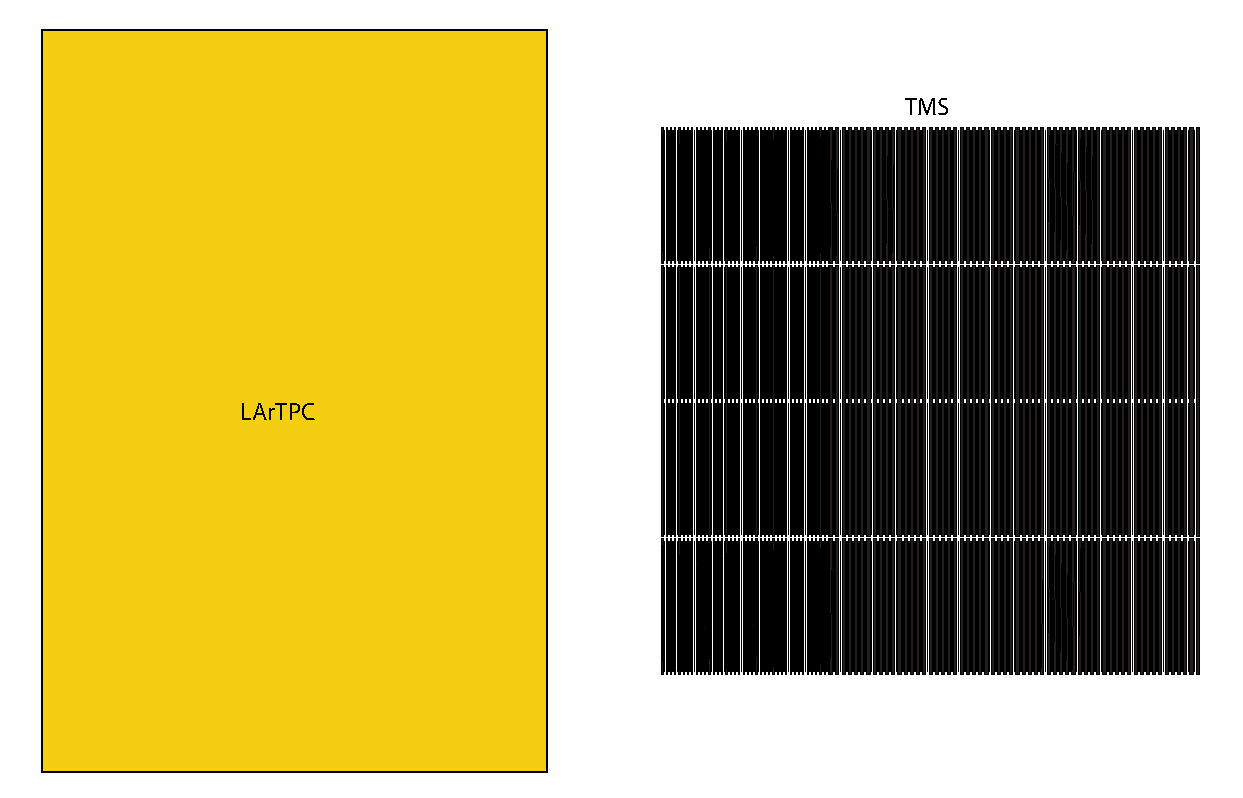
\includegraphics[width=0.8\textwidth]{graphics/tms/Geometry/top_view.pdf}
%\end{dunefigure}
\begin{dunefigure}[GEANT geometery of the \dword{tms} and \dword{ndlar}]{fig:geom_in_hall}
{View of the \dword{tms} geometry (grey) and \dword{ndlar} (orange) in the ND hall. The black line shows the central beam direction which travels left to right in this view. }
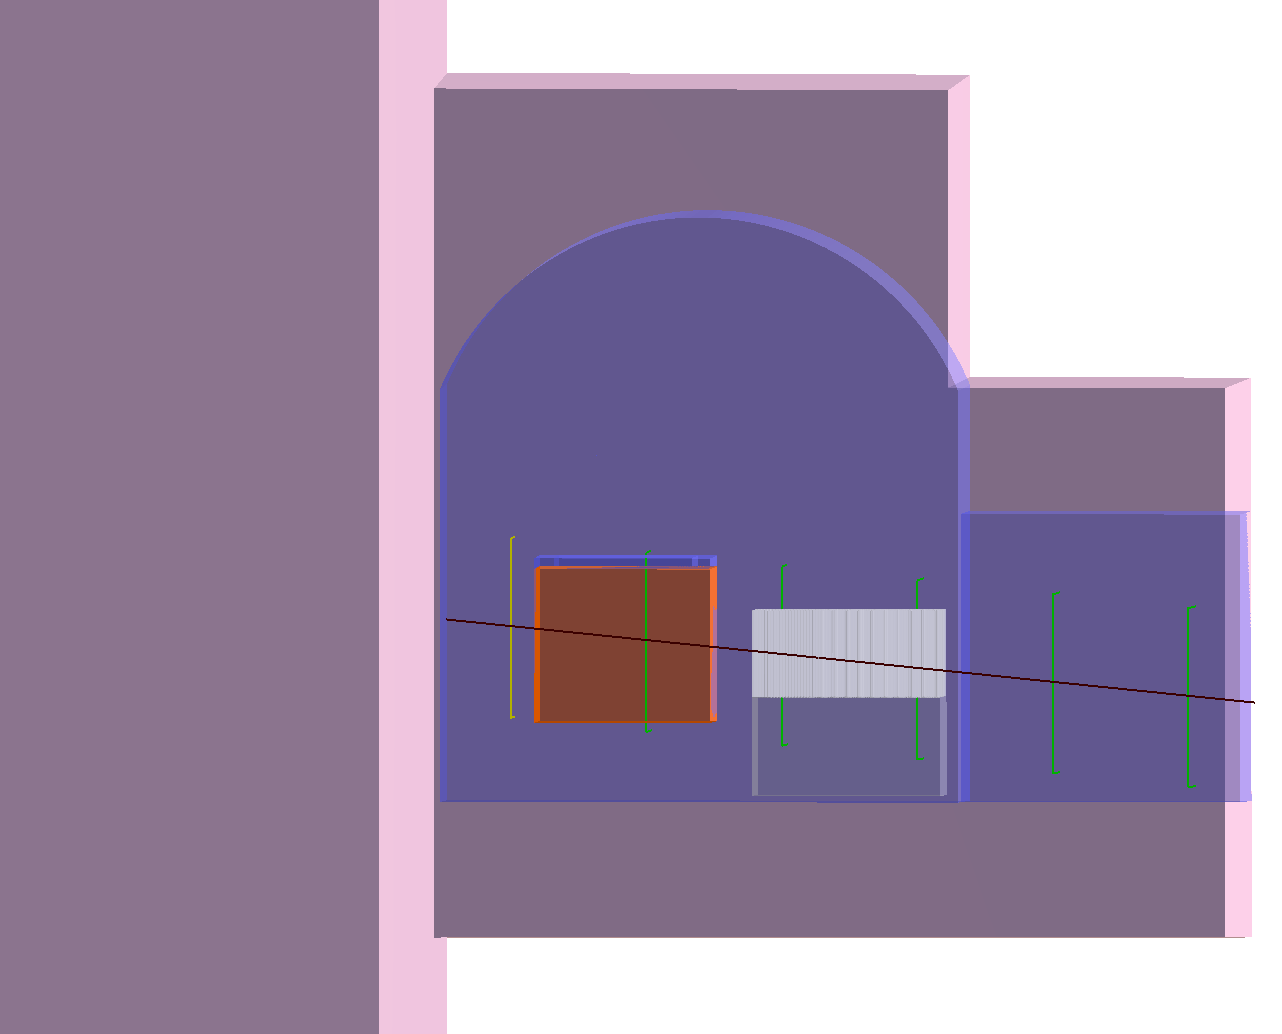
\includegraphics[width=0.8\textwidth]{graphics/tms/Geometry/TMS_LAr.png}
\end{dunefigure}
\begin{dunefigure}[Perspective view of the \dword{tms} and \dword{ndlar}]{fig:geom_3d}
{A perspective view of the \dword{tms} geometry (grey) and \dword{ndlar} (orange). The \dword{ndlar} includes the cryostat in this view.}
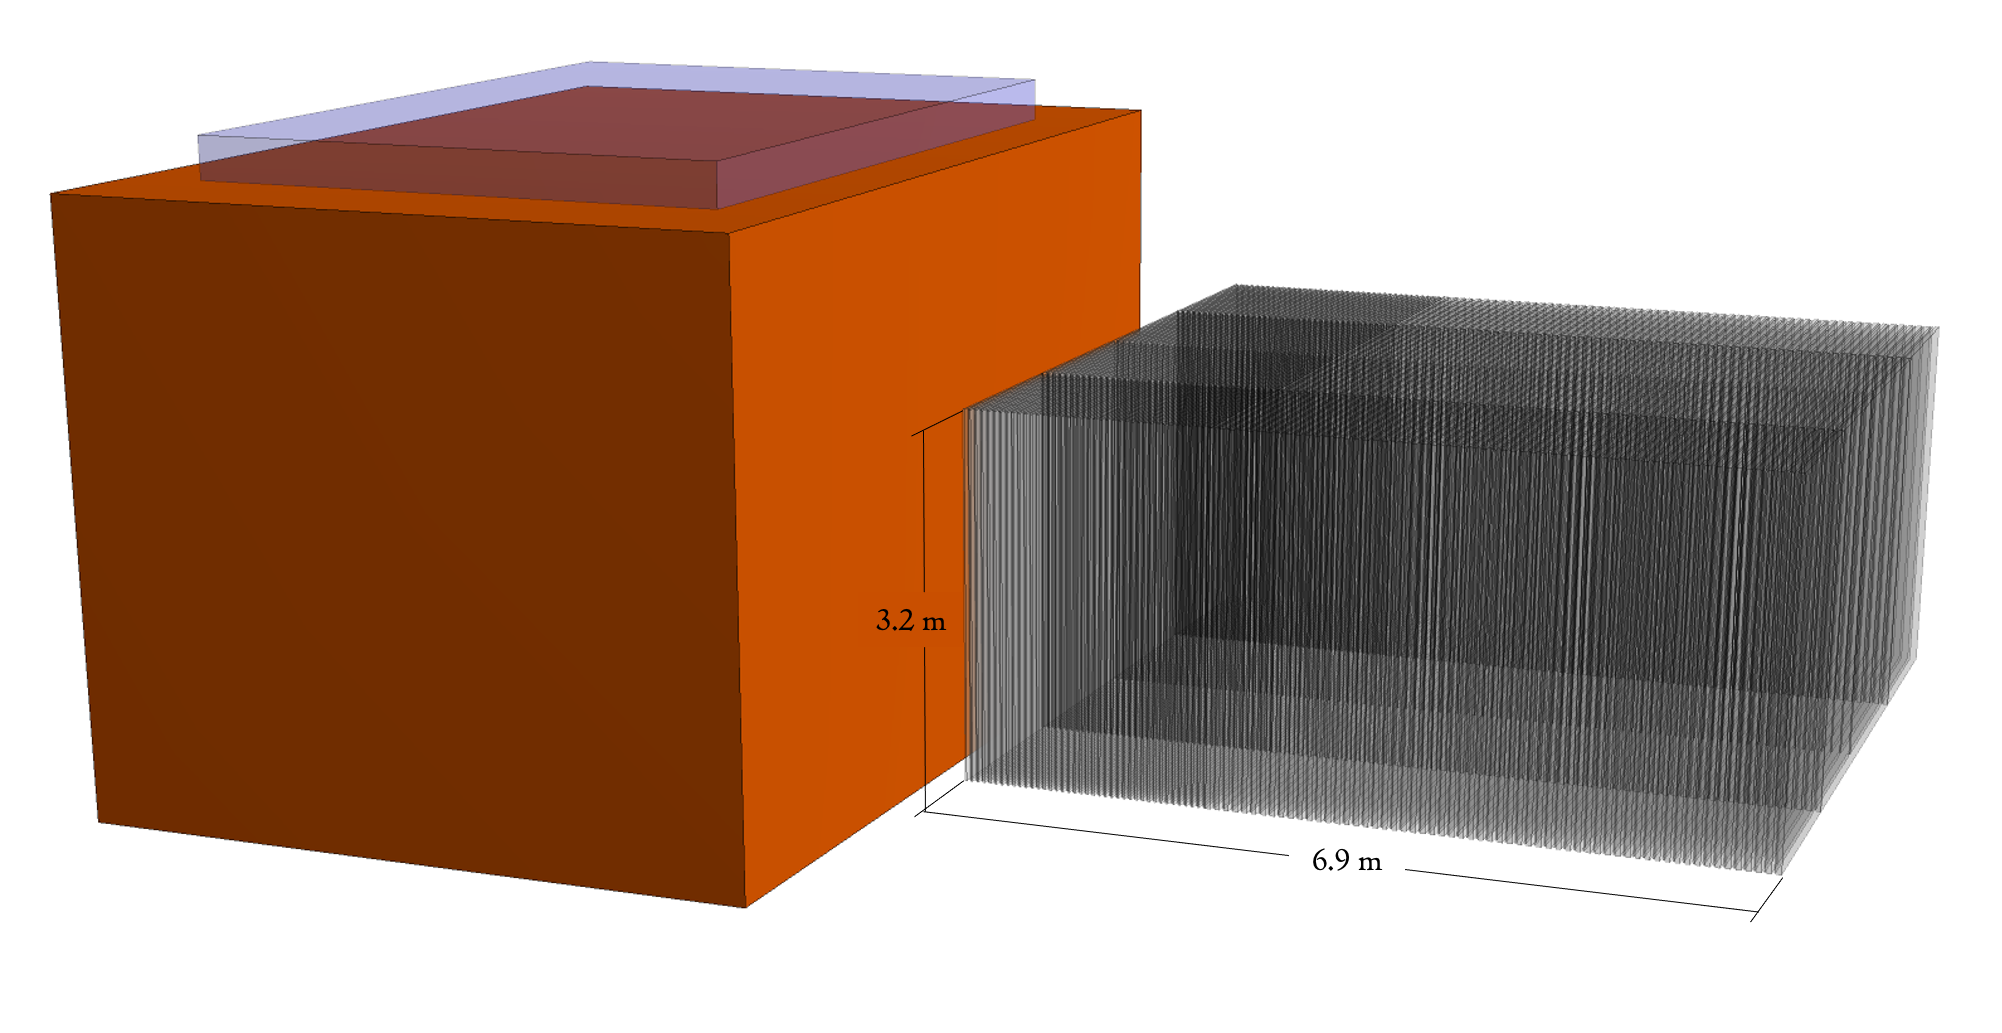
\includegraphics[width=0.8\textwidth]{graphics/tms/Geometry/TMS_LAr_No_Hall.png}
\end{dunefigure}

\subsubsection{Event Gallery}
%\fixme{double check dword usage}
% Clarence's notes:
% Show events stopping in the TMS only
% Show opposite bending of neutrino/anti-neutrino events
% Show some different energies and processes
% Show impossible to reconstruct without TMS
This section presents raw event displays for events contained in the TMS (Figures \ref{fig:evdisplay_QE}-\ref{fig:evdisplay_DIS}, showing the truth hits from the primary lepton and other particles separated. The \dword{ndlar}, gap and \dword{tms} volumes are shown, as are track start, exit, enter and stop positions. Each event display shows the $x-z$ and $y-z$ views, where the $x-z$ view contains the bending from the magnetic field. We also show the incoming neutrino and outgoing lepton energy and ID. These examples emphasize the sign-selection and ranging capabilities of the detector.

% CCQE event with muon E = 2.84 GeV
\begin{dunefigure}[Simulated CCQE event in the \dword{ndlar} and \dword{tms}]{fig:evdisplay_QE}
{A simulated neutrino \dword{cc} \dword{qe} event with $E_\mu=2.84\text{ GeV}$, split into true lepton hits (top row) and other particle hits (middle row), with the $x-z$ view on the left, and $y-z$ view on the right. Each display shows \dword{ndlar} (left), the gap region (middle), and the \dword{tms} (right). Green boxes represent the detector boundaries, and red dashed boxes the fiducial volumes. The green circle is the lepton production point, the red square in \dword{ndlar} is the exit point, the green square is the \dword{tms} entry point, and the red square in the \dword{tms} is the stopping point. This event stops just outside the fiducial volume in $y-z$. True lepton hits are shown zoomed in on the \dword{tms} only (bottom row). The \dword{tms}' plane structure in $z$ is visible, where $z<939\text{ cm}$ shows the region with thin iron plates, and $z>949\text{ cm}$ shows the region with thick iron plates.}
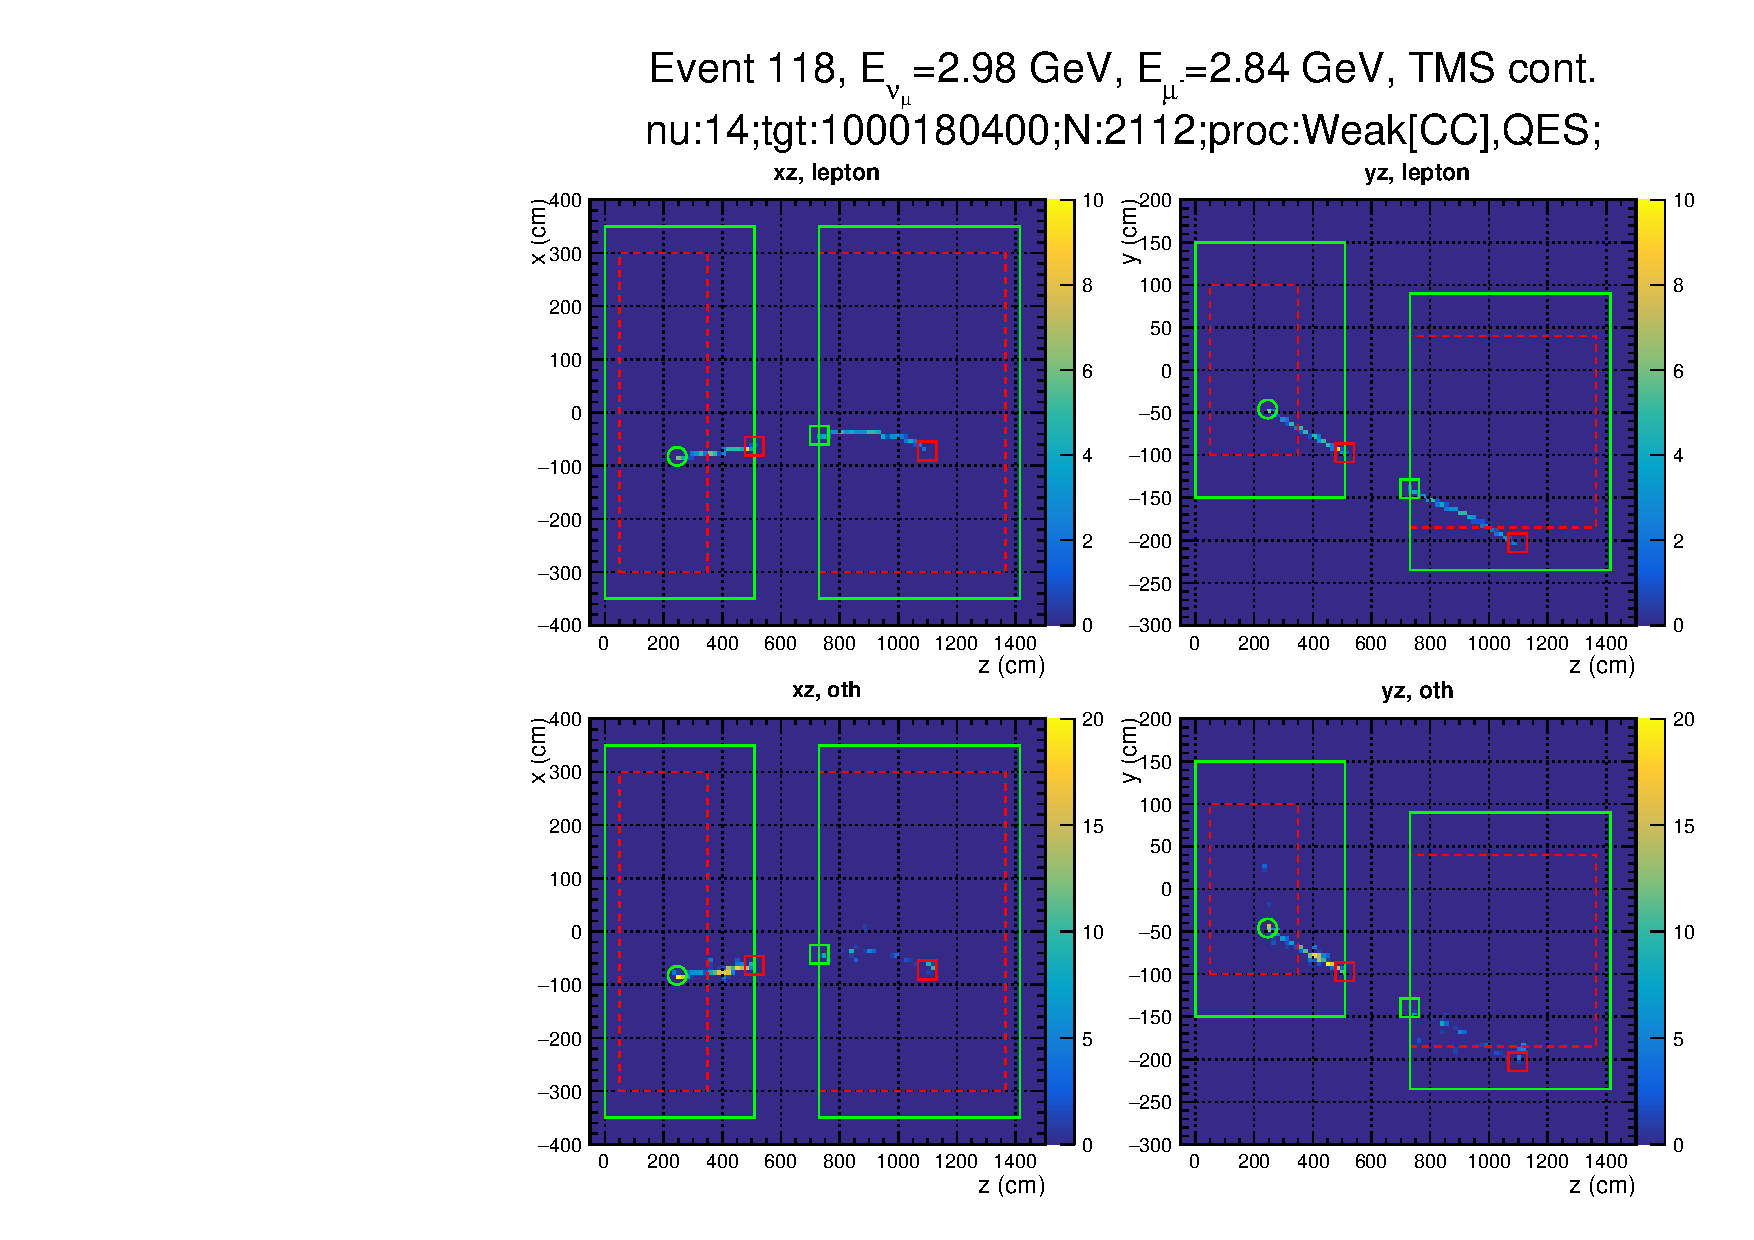
\includegraphics[trim=0 0 0 55, clip, width=0.8\textwidth]{graphics/tms/Simulation/EventDisplay/pg_0009.pdf}
\\[\smallskipamount]
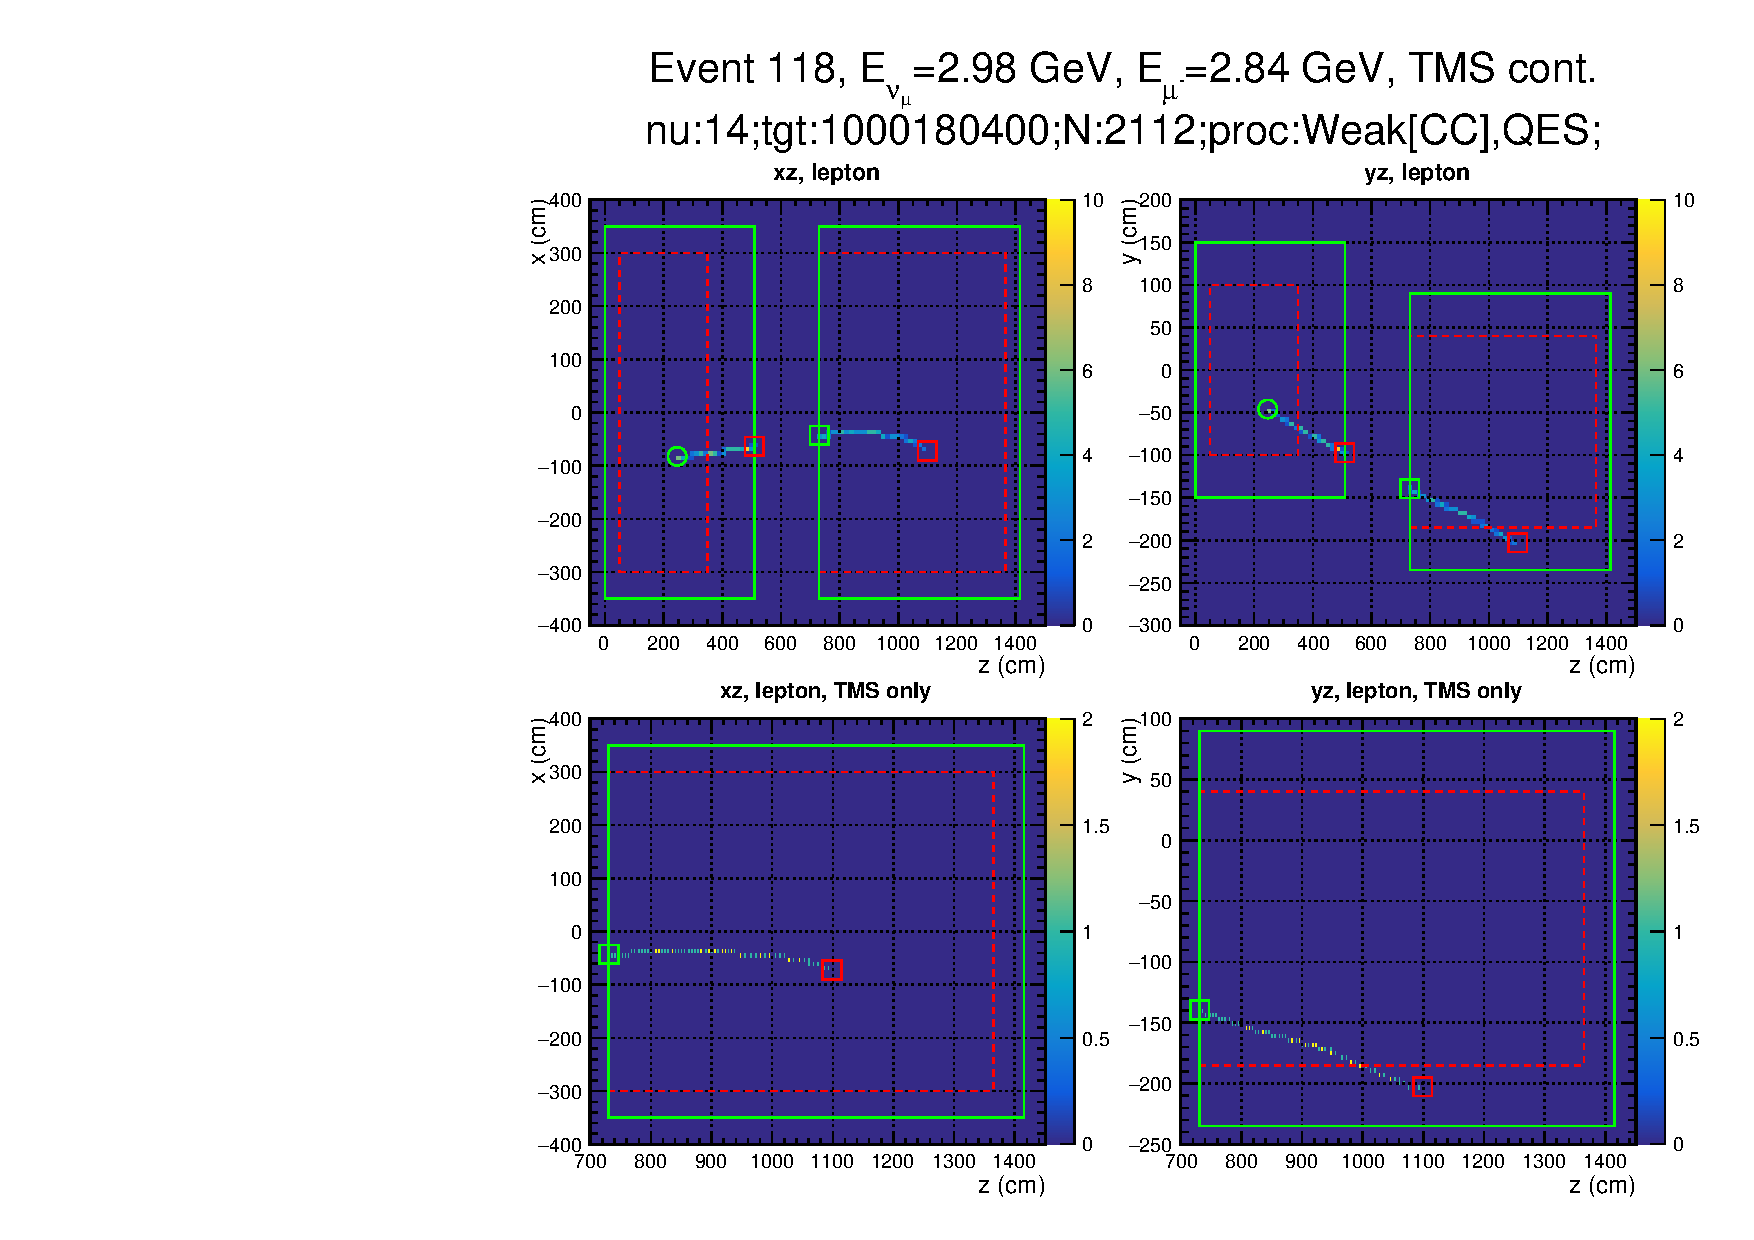
\includegraphics[trim=0 0 0 305, clip, width=0.8\textwidth]{graphics/tms/Simulation/EventDisplay/pg_0010.pdf}
\end{dunefigure}

% Same CCQE event zoomed in on TMS z
%\begin{dunefigure}[Simulated CCQE event in the \dword{ndlar} and \dword{tms}]{}
%{The event in Figure \ref{fig:evdisplay_QE}, showing true lepton hits in both detectors (top row) and zoomed in on the \dword{tms} only (bottom row). The \dword{tms}' plane structure in $z$ is visible in the bottom row, where $z<939\text{ cm}$ shows the region with thin iron plates, and $z>949\text{ cm}$ shows the region with thick iron plates.}
%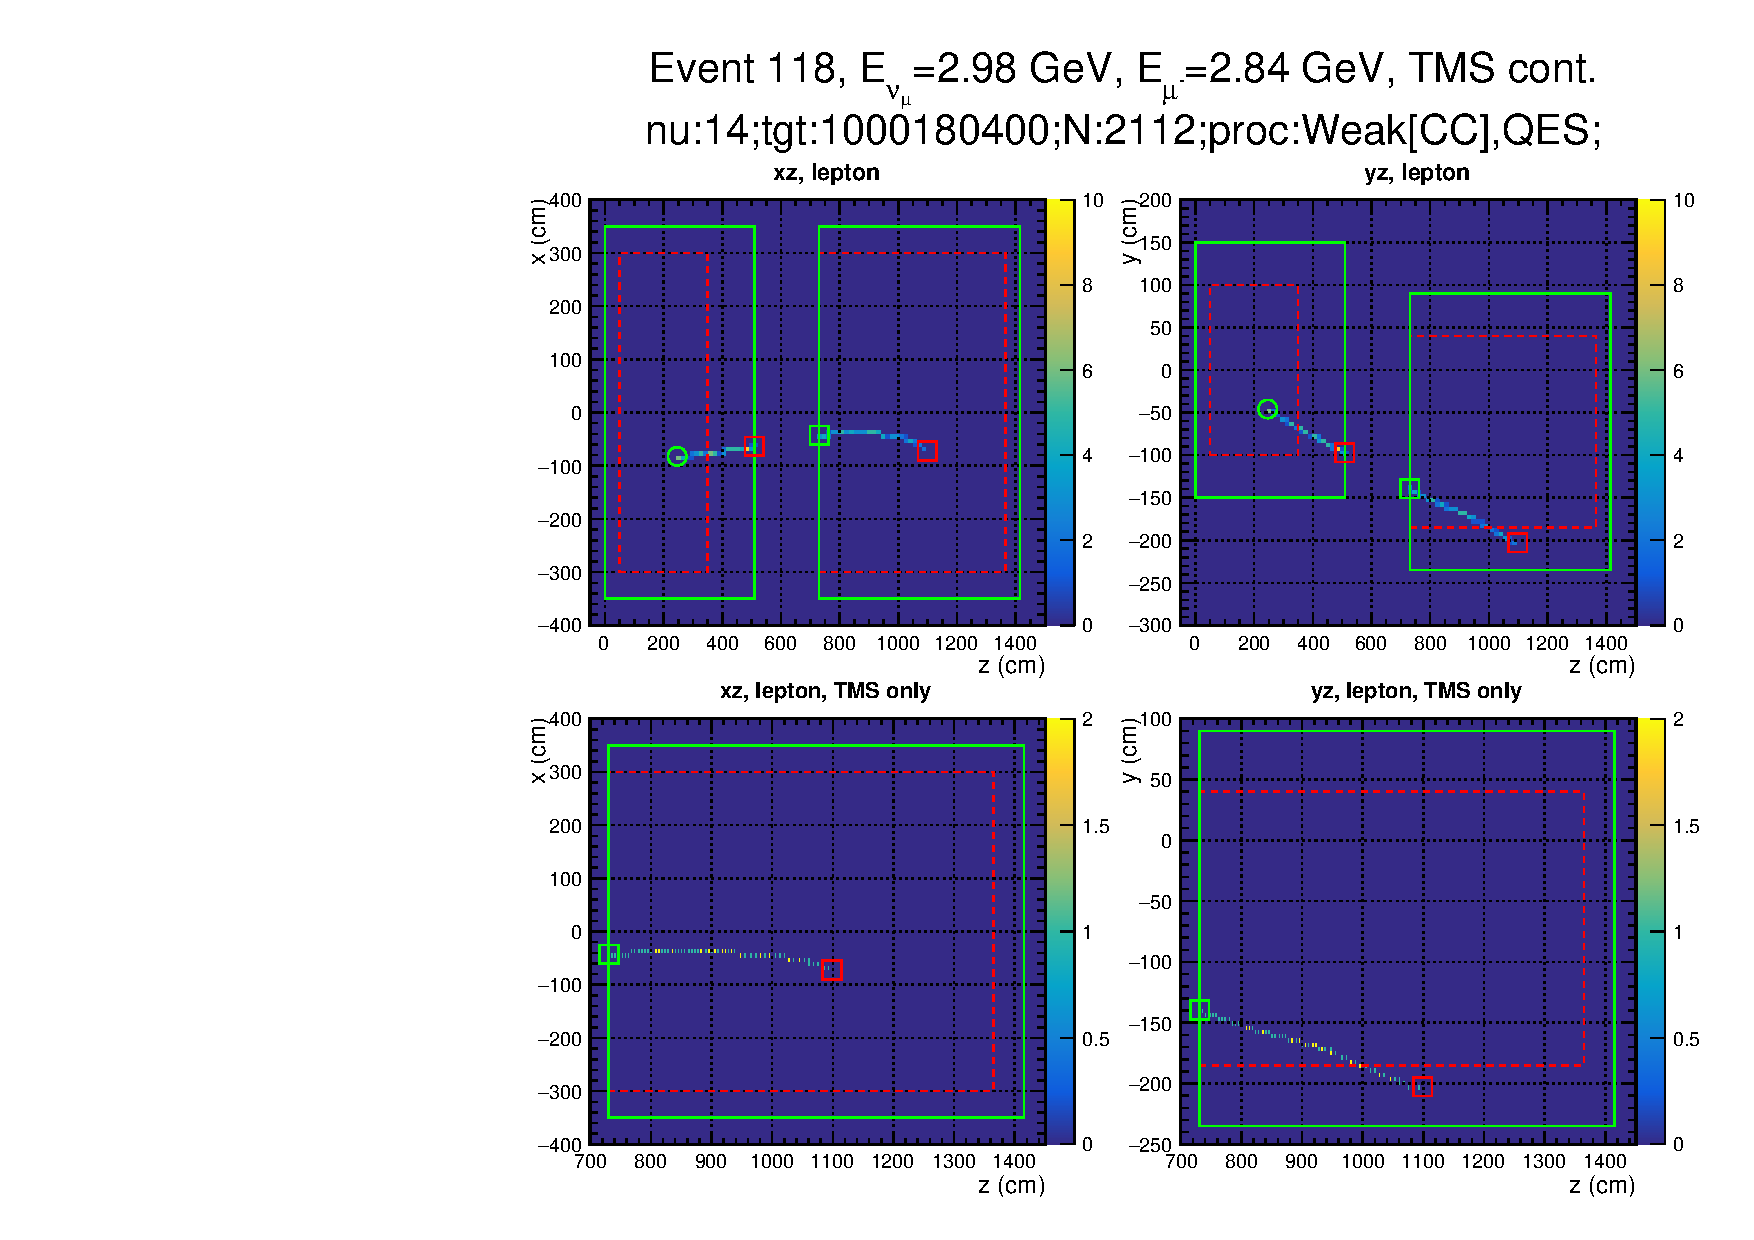
\includegraphics[trim=0 0 0 55, clip, %width=0.8\textwidth]{graphics/tms/Simulation/EventDisplay/pg_0010.pdf}
%\end{dunefigure}

% 2p2h anti-neutrino event with similar muon energy, displaying bending
\begin{dunefigure}[Simulated 2p2h event in the \dword{ndlar} and \dword{tms}]{fig:evdisplay_antinu}
{A simulated anti-neutrino \dword{2p2h} event with $E_\mu=2.68\text{ GeV}$, split into true lepton hits (top row) and other particle hits (middle row), with the $x-z$ view on the left, and $y-z$ view on the right. Compared to the CCQE event in Figure \ref{fig:evdisplay_QE} the \dword{tms} bends the muon in the opposite direction, enabling sign-selection. True lepton hits are shown zoomed in on the \dword{tms} only (bottom row).}
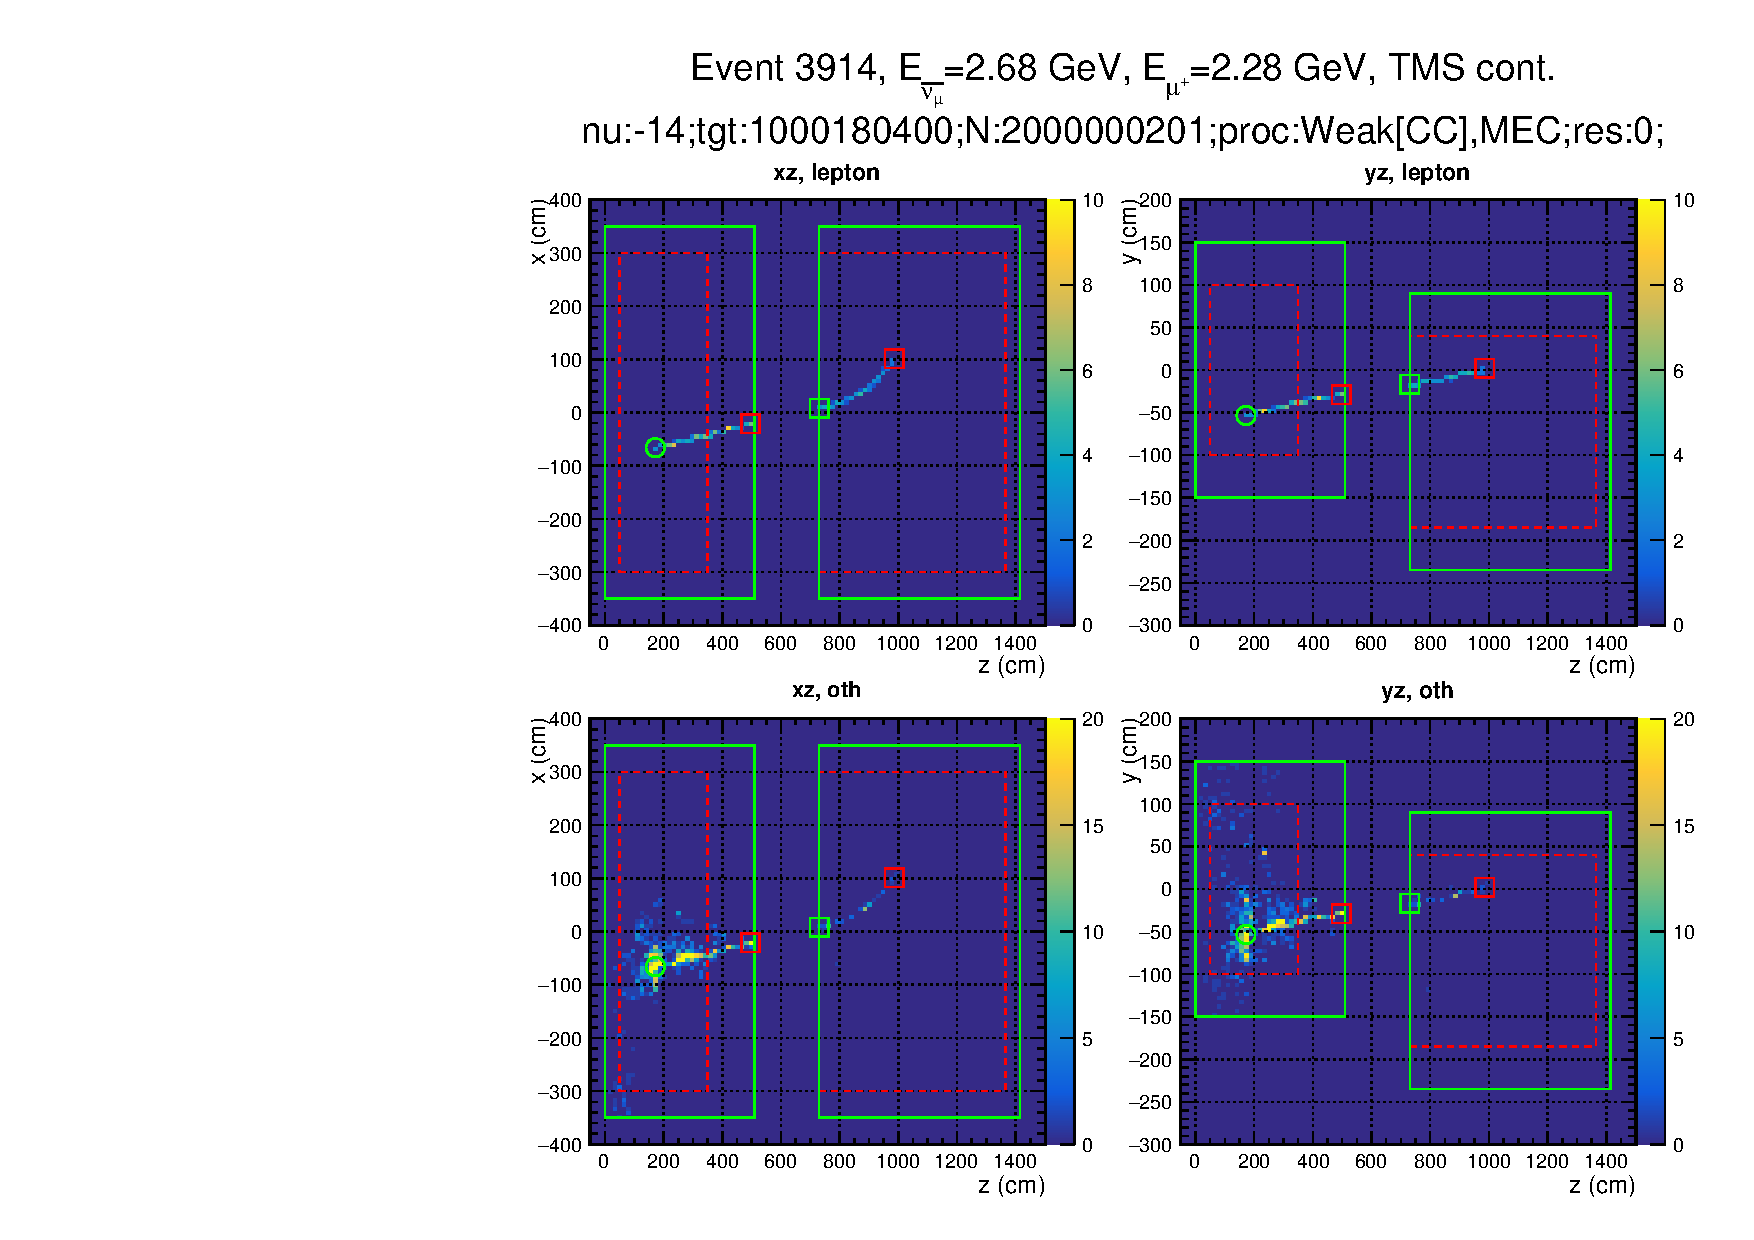
\includegraphics[trim=0 0 0 55, clip,width=0.8\textwidth]{graphics/tms/Simulation/EventDisplay/pg_0011.pdf}
\\[\smallskipamount]
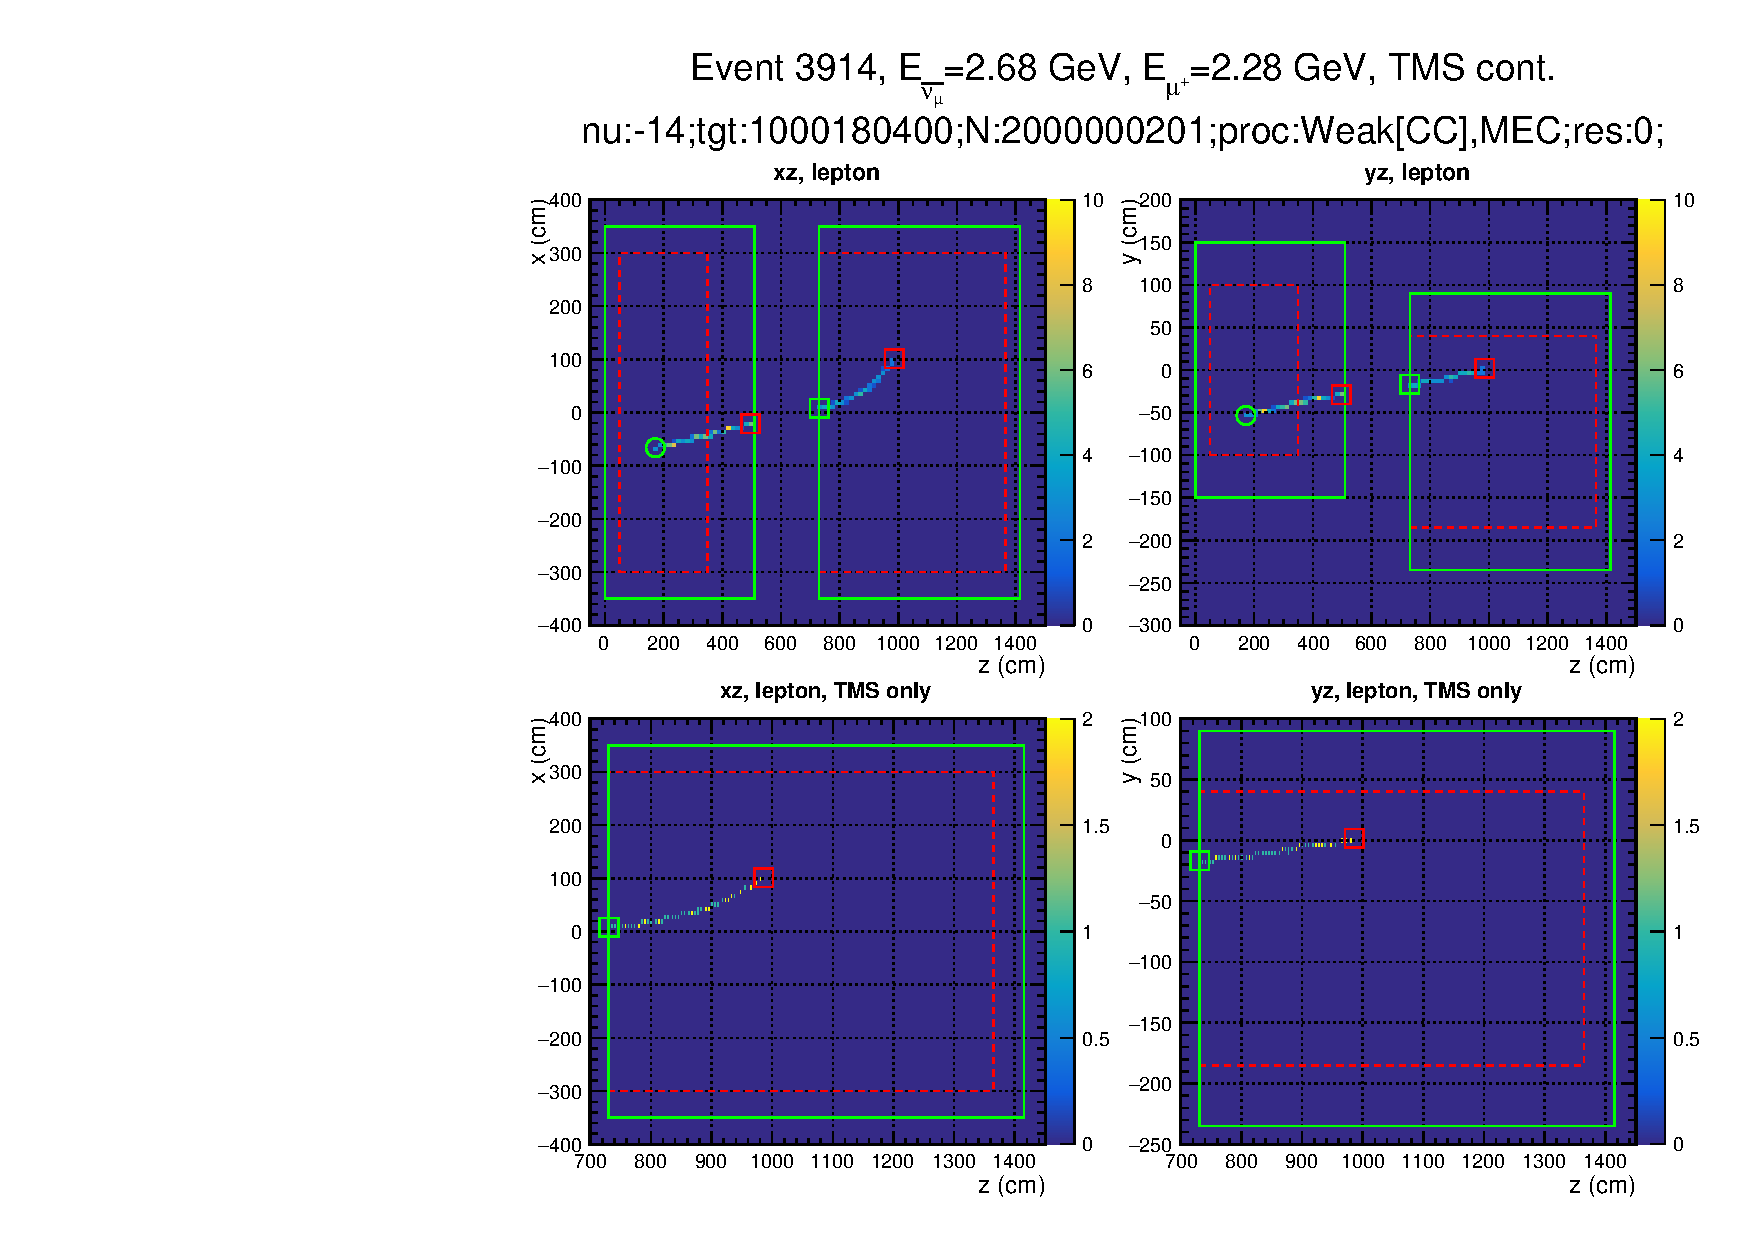
\includegraphics[trim=0 0 0 305, clip,width=0.8\textwidth]{graphics/tms/Simulation/EventDisplay/pg_0012.pdf}
\end{dunefigure}

% Same 2p2h anti-neutrino event, showing zoomed in on TMS region
%\begin{dunefigure}[Simulated 2p2h event in the \dword{ndlar} and \dword{tms}]{}
%{The event in Figure \ref{fig:evdisplay_antinu}, showing true lepton hits in both detectors (top row) and zoomed in on the \dword{tms} only (bottom row).}
%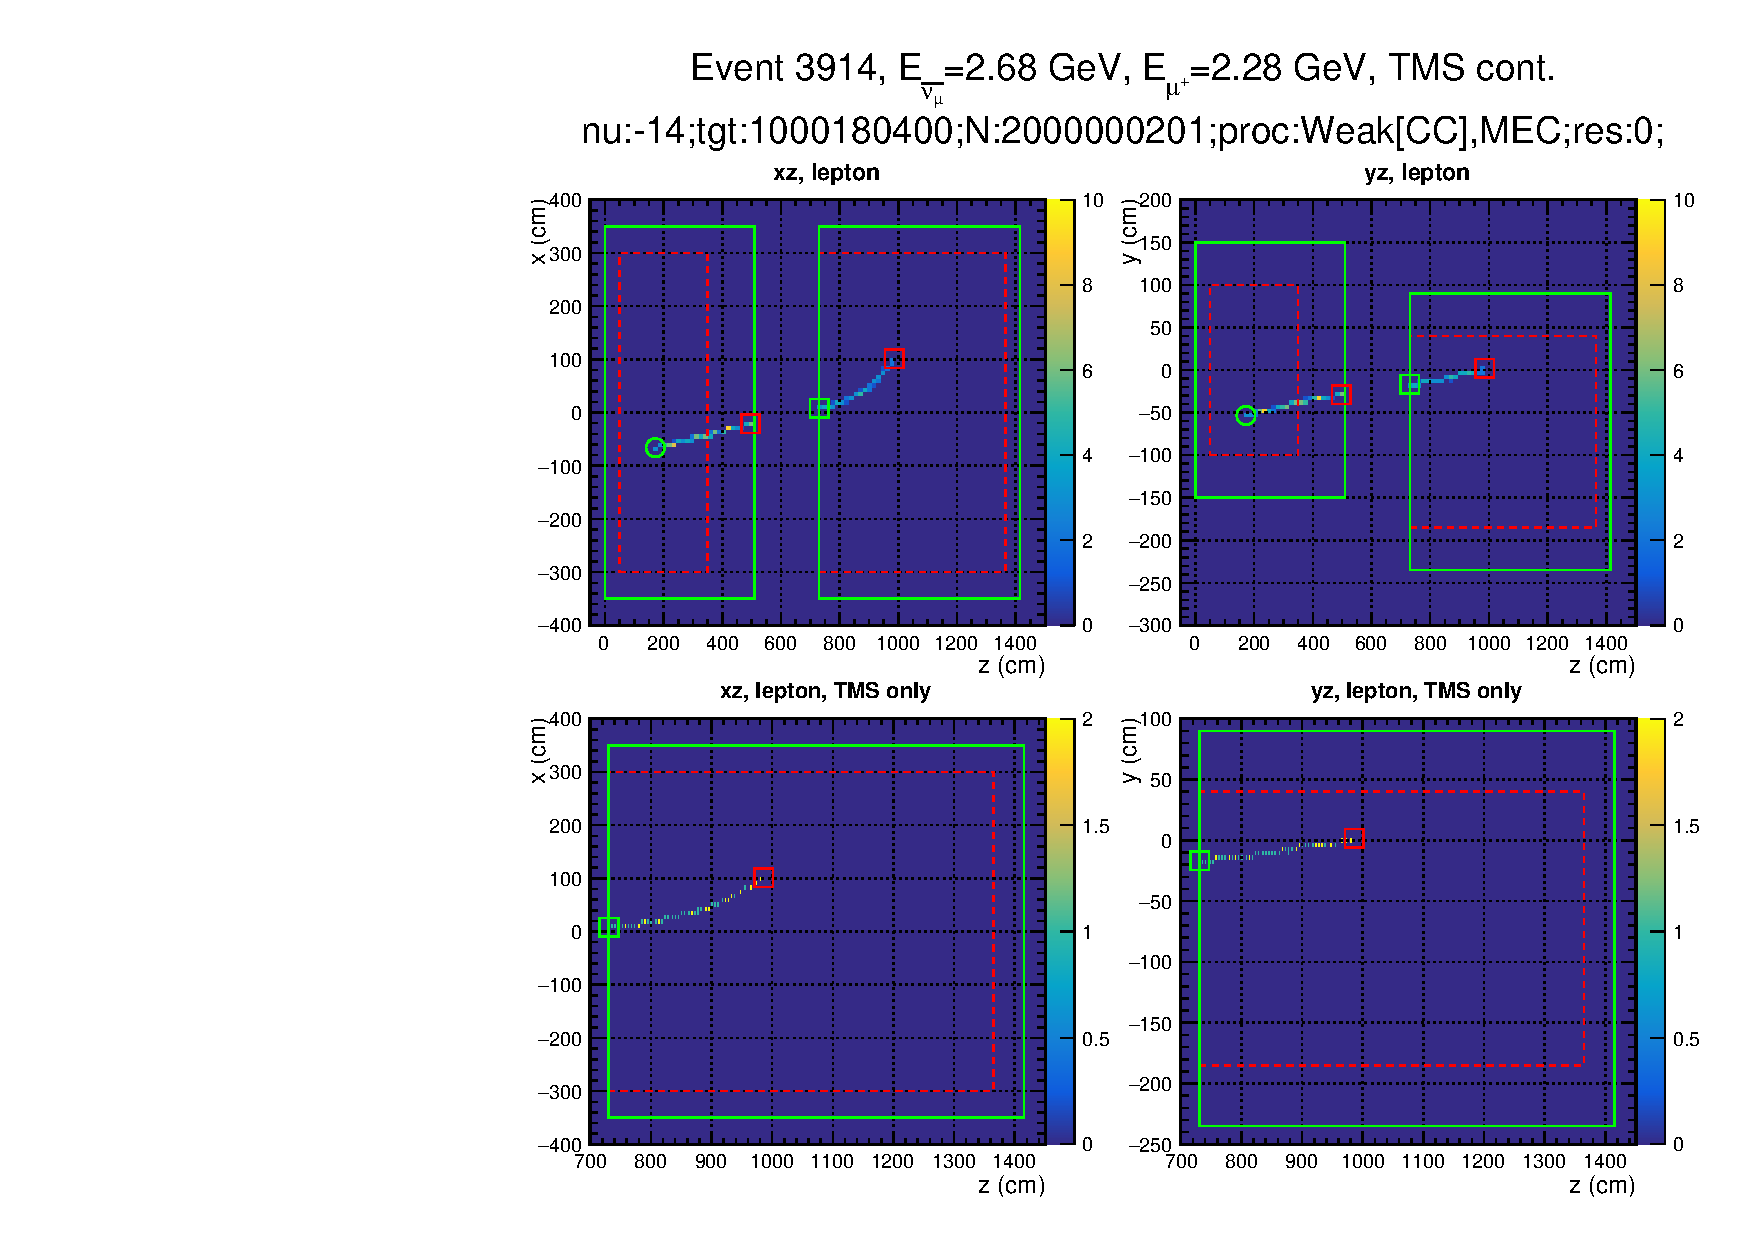
\includegraphics[trim=0 0 0 55, %clip,width=0.8\textwidth]{graphics/tms/Simulation/EventDisplay/pg_0012.pdf}
%\end{dunefigure}

% A higher energy event, giving an idea of the top muon energy range for the current design (~5 GeV)
% Also shows that none of the showers in ArgonCube make it to the TMS
\begin{dunefigure}[Simulated DIS event in the \dword{ndlar} and \dword{tms}]{fig:evdisplay_DIS}
{A simulated neutrino \dword{dis} event with $E_\mu=4.60\text{ GeV}$ and sizeable hadronic energy ($E_{had}\sim2.2\text{ GeV}$), which traverses most of the \dword{tms} in $z$. The particle is traveling in the outer steel plates here. The hadronic showers and sizeable muon kinetic energy in the \dword{ndlar} makes muon identification troublesome without the \dword{tms}.}
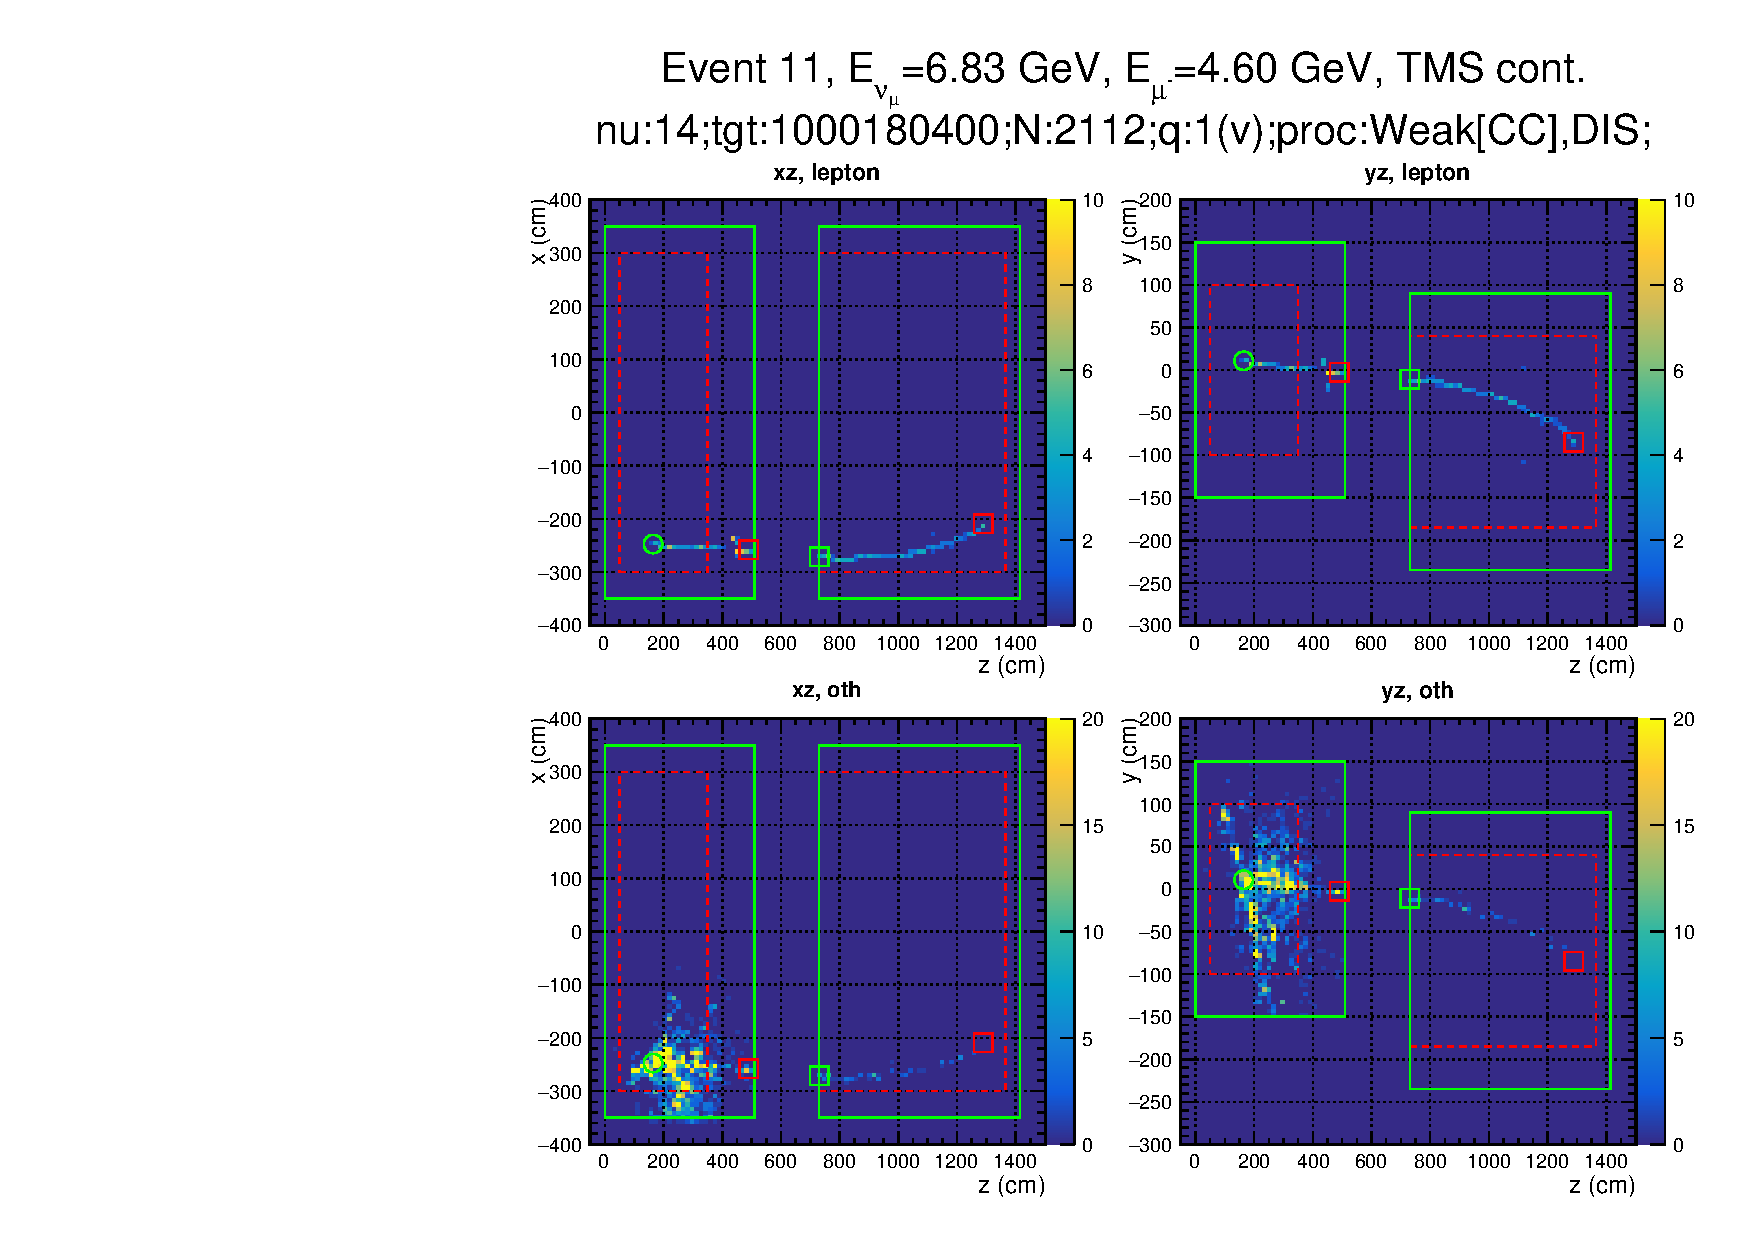
\includegraphics[trim=0 0 0 55, clip,width=0.8\textwidth]{graphics/tms/Simulation/EventDisplay/pg_0001.pdf}
\end{dunefigure}

% Probably useful to flush pictures out here
\clearpage

\subsubsection{Acceptance}

This section presents preliminary studies using the generated neutrino interactions in the \dword{ndlar} active volume. We calculate the number of events with a true muon contained in the \dword{ndlar} and \dword{tms} detectors and compare it to the total events with a true muon generated on the active \dword{ndlar} volume. We use the true generated positions to calculate the acceptances as a full reconstruction is not yet available. We make no fiducial volume requirements on the \dword{ndlar} interaction; only that the interaction occurs on the active \dword{ndlar} volume. This study demonstrates the kinematic coverage of the \dword{ndlar}+\dword{tms} system, which is by design comparable to or beyond the \dword{ndlar}+\dword{ndgar} system and therefore satisfies DUNE physics requires for initial running. The efficiencies reported below are sculpted largely by detector effects.   

The \dword{tms} is directly downstream of the \dword{ndlar}, and so greatly improves the forward-going acceptance with the combined \dword{ndlar}+\dword{tms} system. Figure \ref{fig:eff_th} shows the acceptance as a function of the muon angle, $\theta_{\nu,\mu}$, relative to the average neutrino direction. We see the \dword{tms} does well to compensate for the \dword{ndlar} acceptance at low $\theta_{\nu,\mu}$, and has a maximum acceptance of $\sim45\%$ at $\theta_{\nu,\mu}\sim10\degree$. The lowest acceptance for the combined LAr+TMS system is at $\theta_{\nu,\mu}\sim 30\degree$, at which it is 30\%.
% acceptance in muon/neutri  no angle
\begin{dunefigure}[Acceptance as a function of muon angle]{fig:eff_th}
{Acceptance the \dword{ndlar}, \dword{tms} and combined system in $\theta_{\nu,\mu}$. Left shows the events starting in the \dword{ndlar} and contained in the different detectors, compared with all events. Right shows the ratio of each category relative the total. All events in this plot had muons originating in the liquid argon: ``LAr contained'' and ``TMS contained'' refer to the subdetector where the muon stops.}
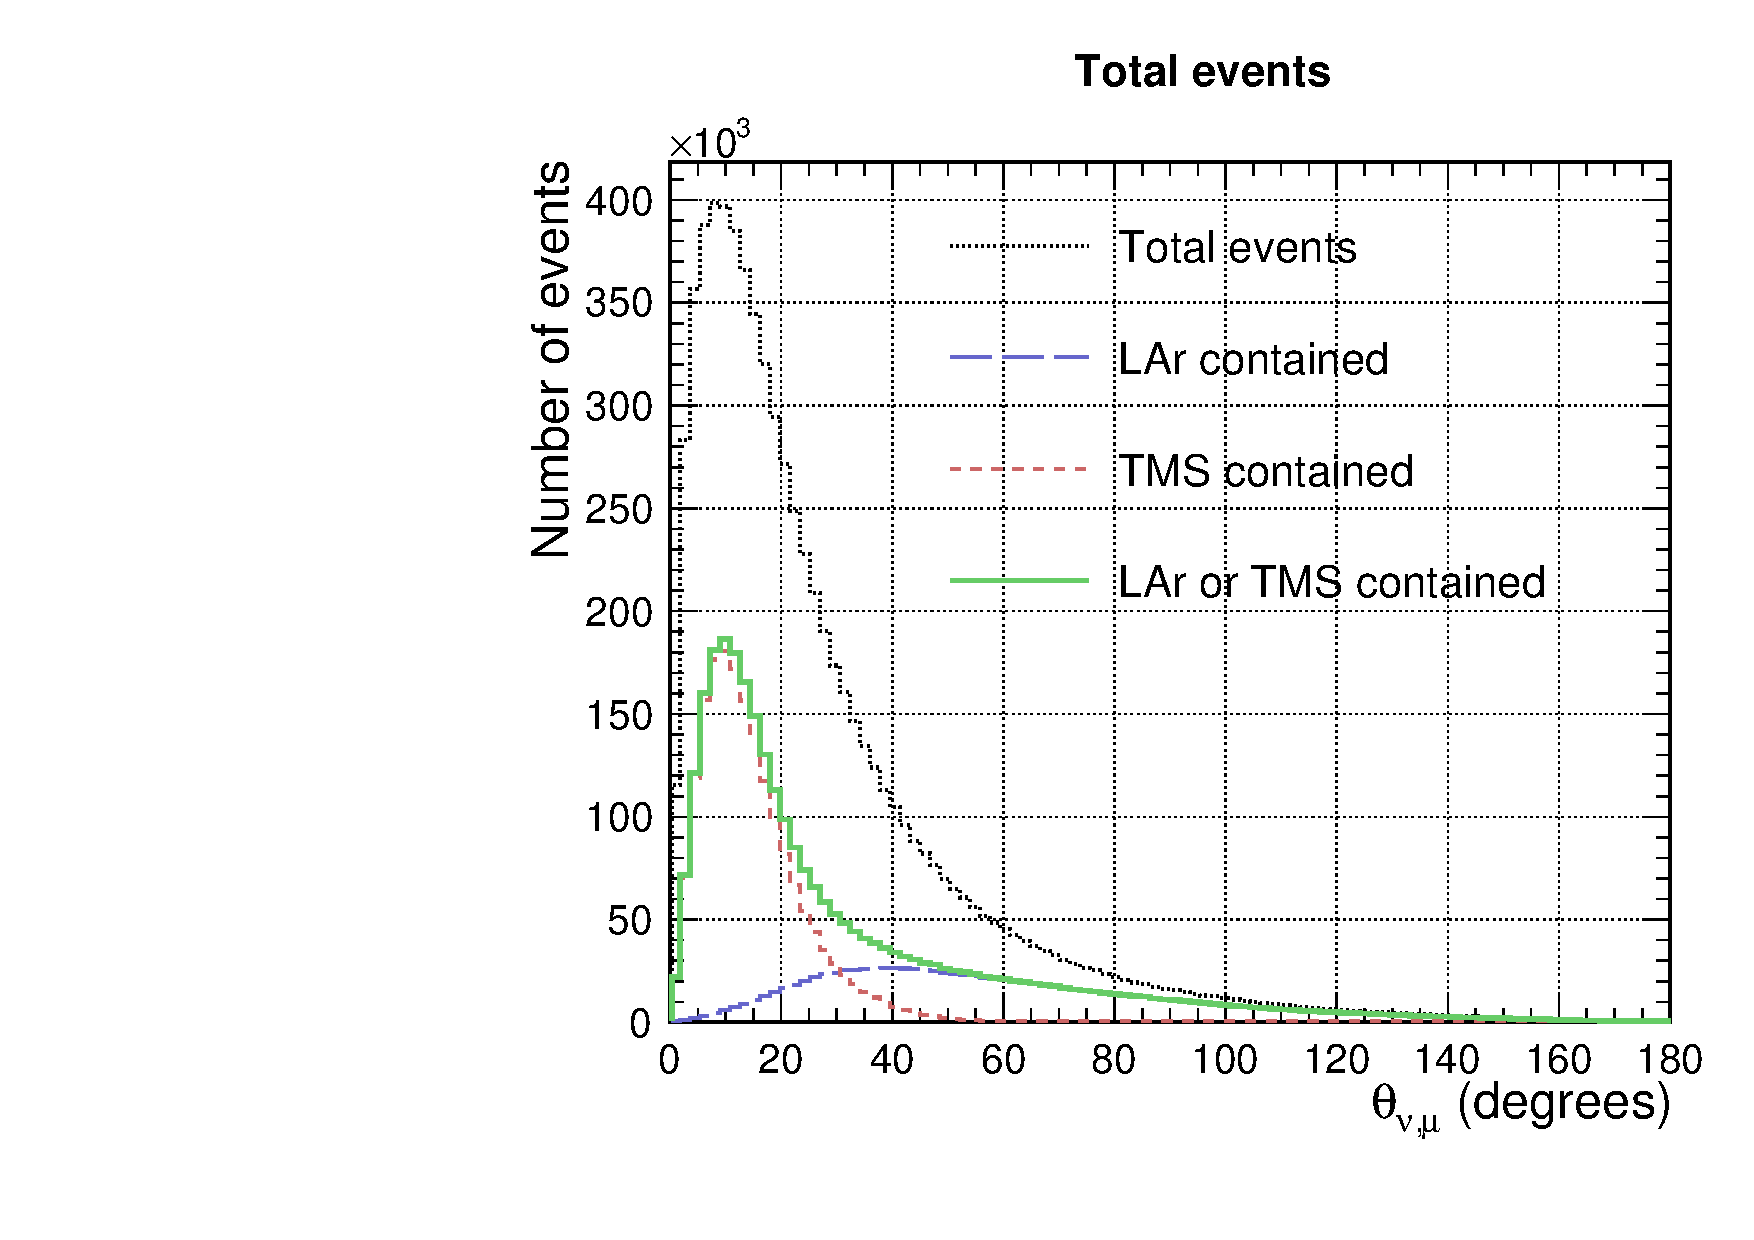
\includegraphics[width=0.49\textwidth, clip, trim={0mm 0mm 0mm 10mm}]{graphics/tms/Simulation/Efficiency/eff_theta.pdf} 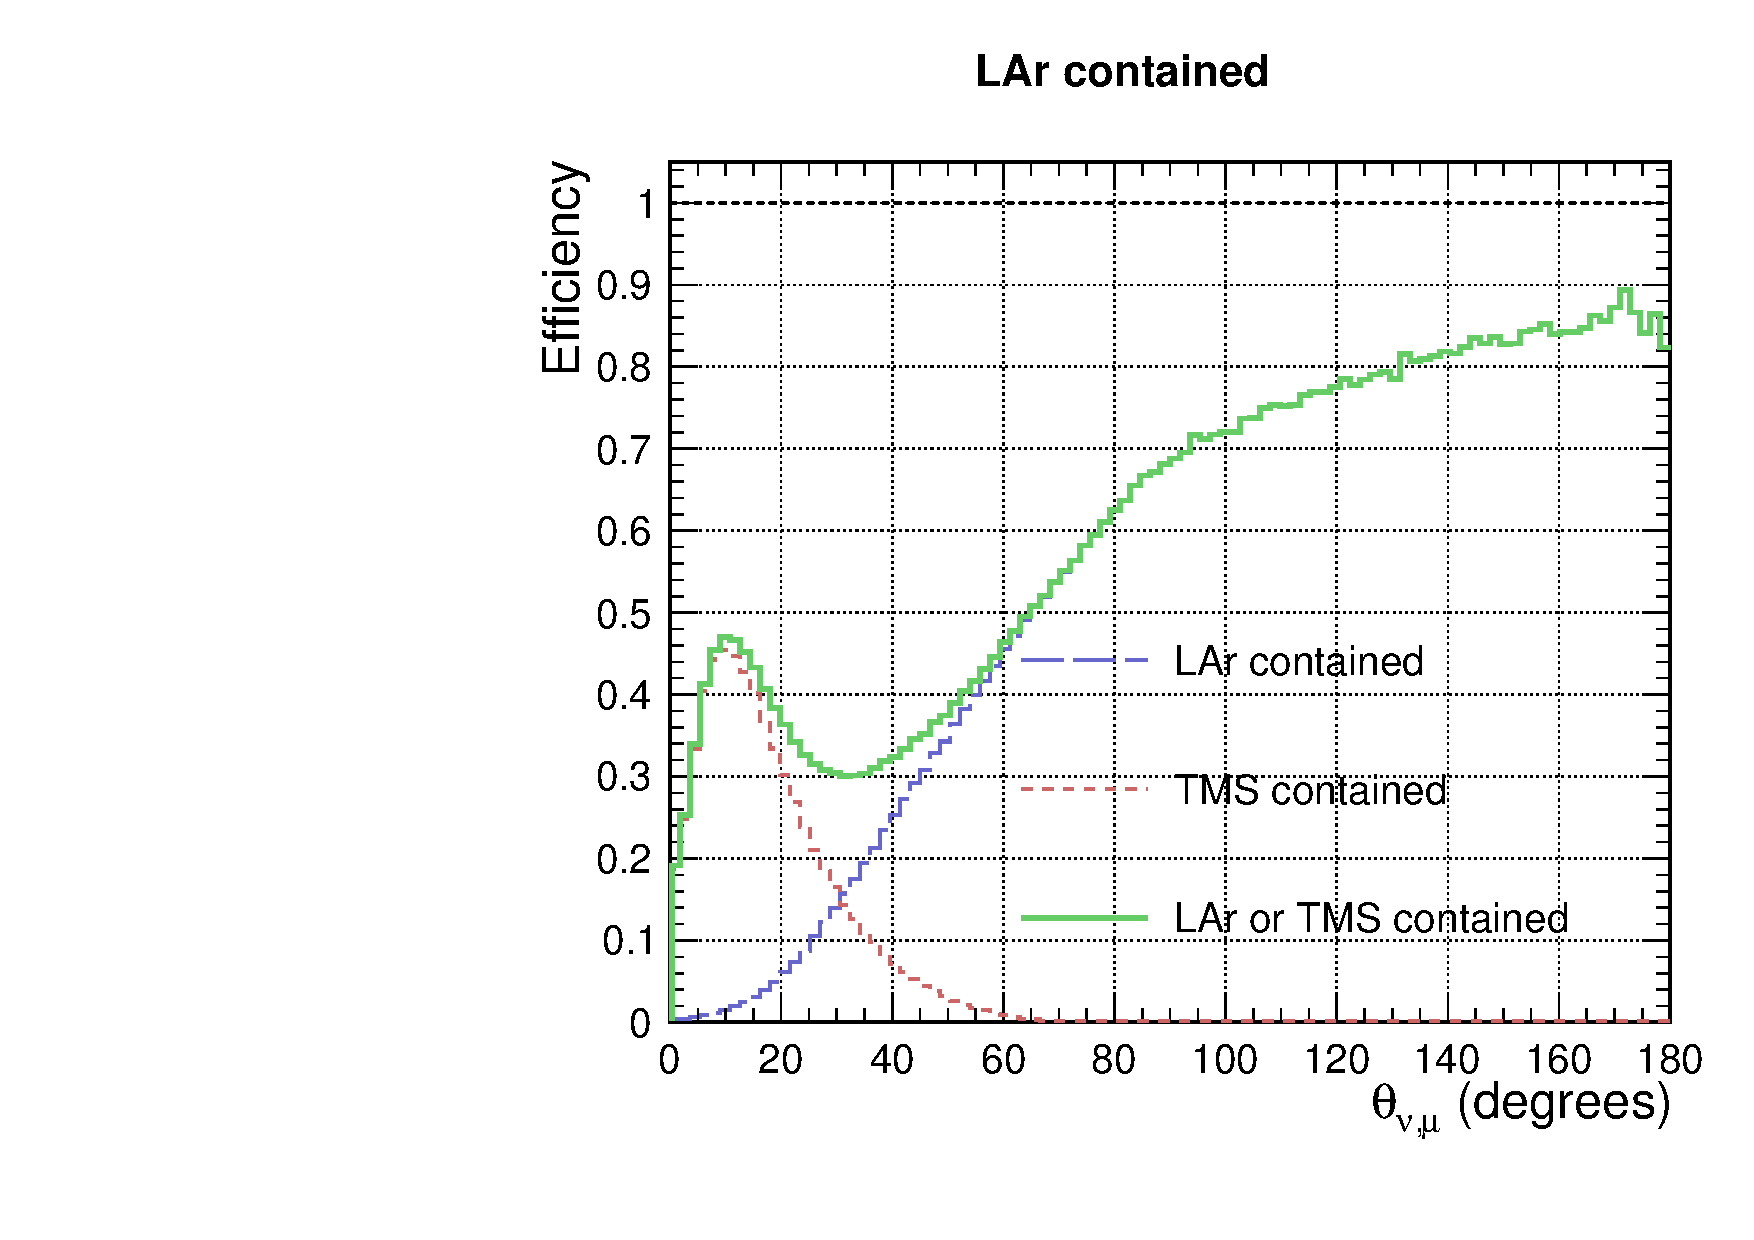
\includegraphics[width=0.49\textwidth, clip, trim={0mm 0mm 0mm 10mm}]{graphics/tms/Simulation/Efficiency/eff_theta_ratio.pdf}
\end{dunefigure}

Figure \ref{fig:eff_enu} shows the acceptance as a function of incoming neutrino energy ($E_\nu$) in \dword{fhc}. We see the \dword{ndlar} performing well at low neutrino energy, with $>40\%$ efficiency when $E_\nu < 1 \text{ GeV}$. It rapidly falls with increasing neutrino energy, and is $\sim15\%$ at the $E_\nu\sim 2.5\text{ GeV}$ peak. The \dword{tms} acceptance rises steadily as the \dword{ndlar} acceptance drops, leading to a combined flat acceptance of $\sim45\%$ between $2.0<E_\nu<4.0\text{ GeV}$. Figure \ref{fig:eff_pt_pl} show this acceptance in muon transverse and longitudinal momentum-space.

% Overall acceptance in neutrino energy
\begin{dunefigure}[Acceptance as a function of neutrino energy]{fig:eff_enu}
{Acceptance of the \dword{ndlar}, \dword{tms} and combined system in $E_\nu^\text{True}$. Left shows the events starting in the \dword{ndlar} and contained in the different detectors, compared with all events. Right shows the ratio of each category relative the total.}
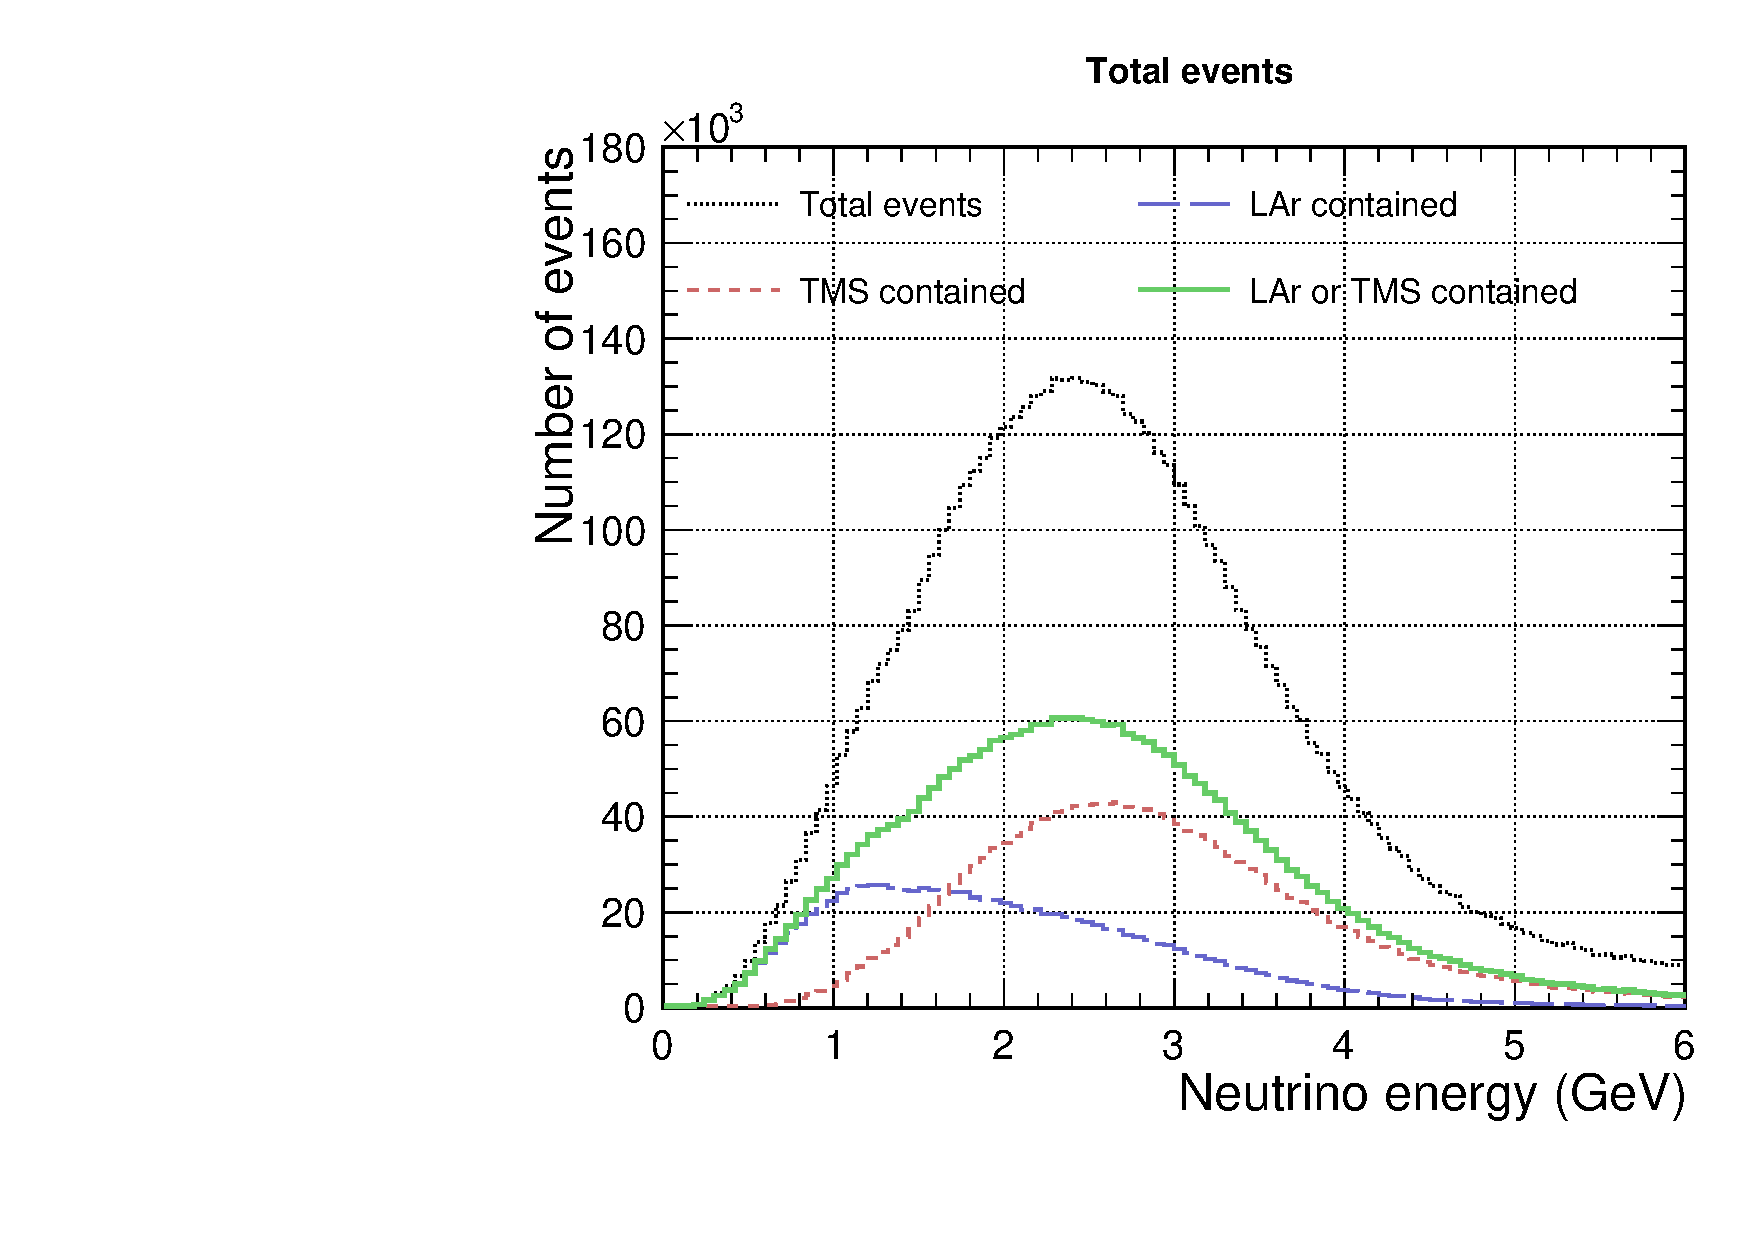
\includegraphics[width=0.49\textwidth, clip, trim={0mm 0mm 0mm 10mm}]{graphics/tms/Simulation/Efficiency/eff.pdf} 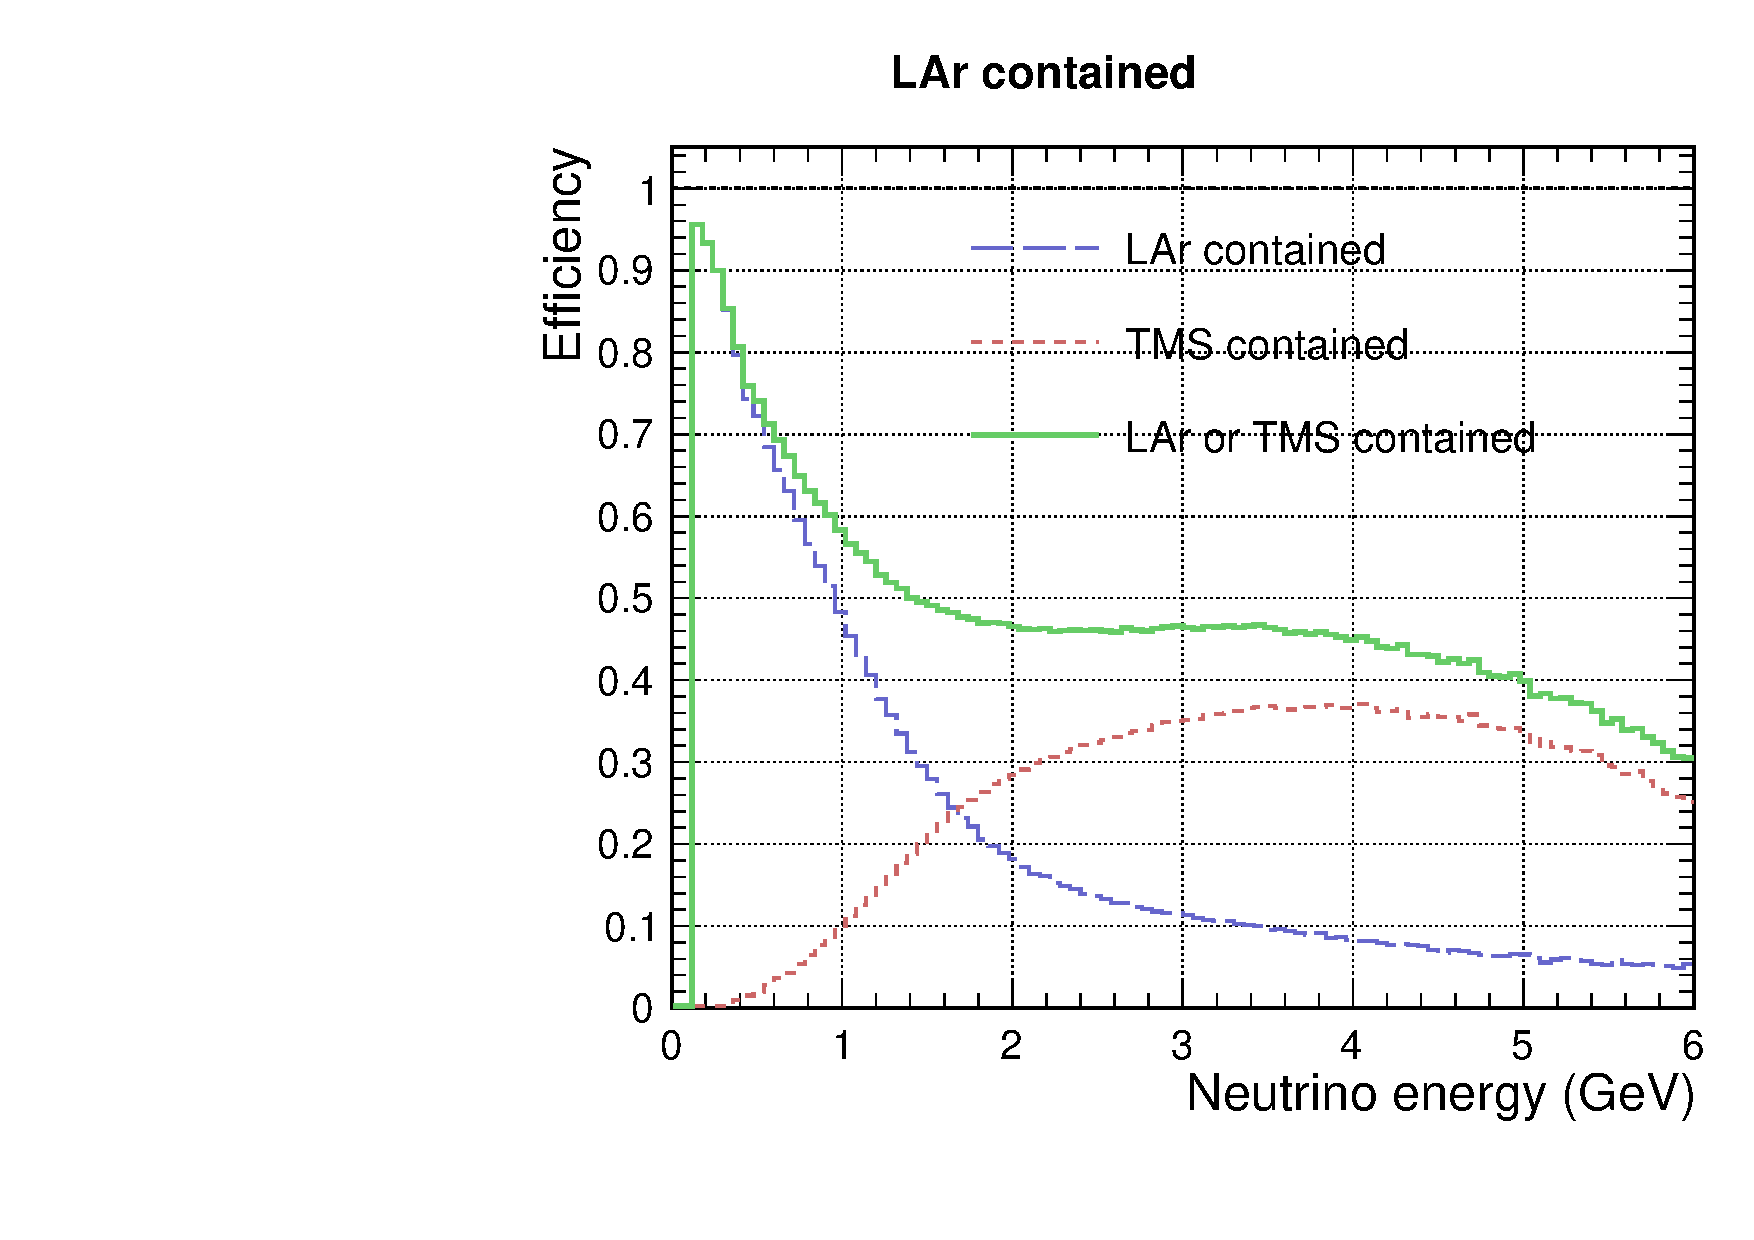
\includegraphics[width=0.49\textwidth, clip, trim={0mm 0mm 0mm 10mm}]{graphics/tms/Simulation/Efficiency/eff_ratio.pdf}
\end{dunefigure}

Figure \ref{fig:eff_pt_pl} shows the same \dword{ndlar}+\dword{tms} acceptance projected onto the transverse and longitudinal momentum of the muon. The acceptance is high below 0.5 GeV/c of transverse momentum due to the downstream location of the TMS. The longitudinal momentum acceptance abruptly falls around 5 GeV/c due to requiring the muon to be stopping in the \dword{tms}, with very low acceptance beyond 6 GeV/c.

\begin{dunefigure}[Fractional acceptance for muon transverse and longitudinal momentum.]{fig:eff_pt_pl}
{Acceptance of the \dword{ndlar}+\dword{tms} detectors in muon transverse and longitudinal momentum.}
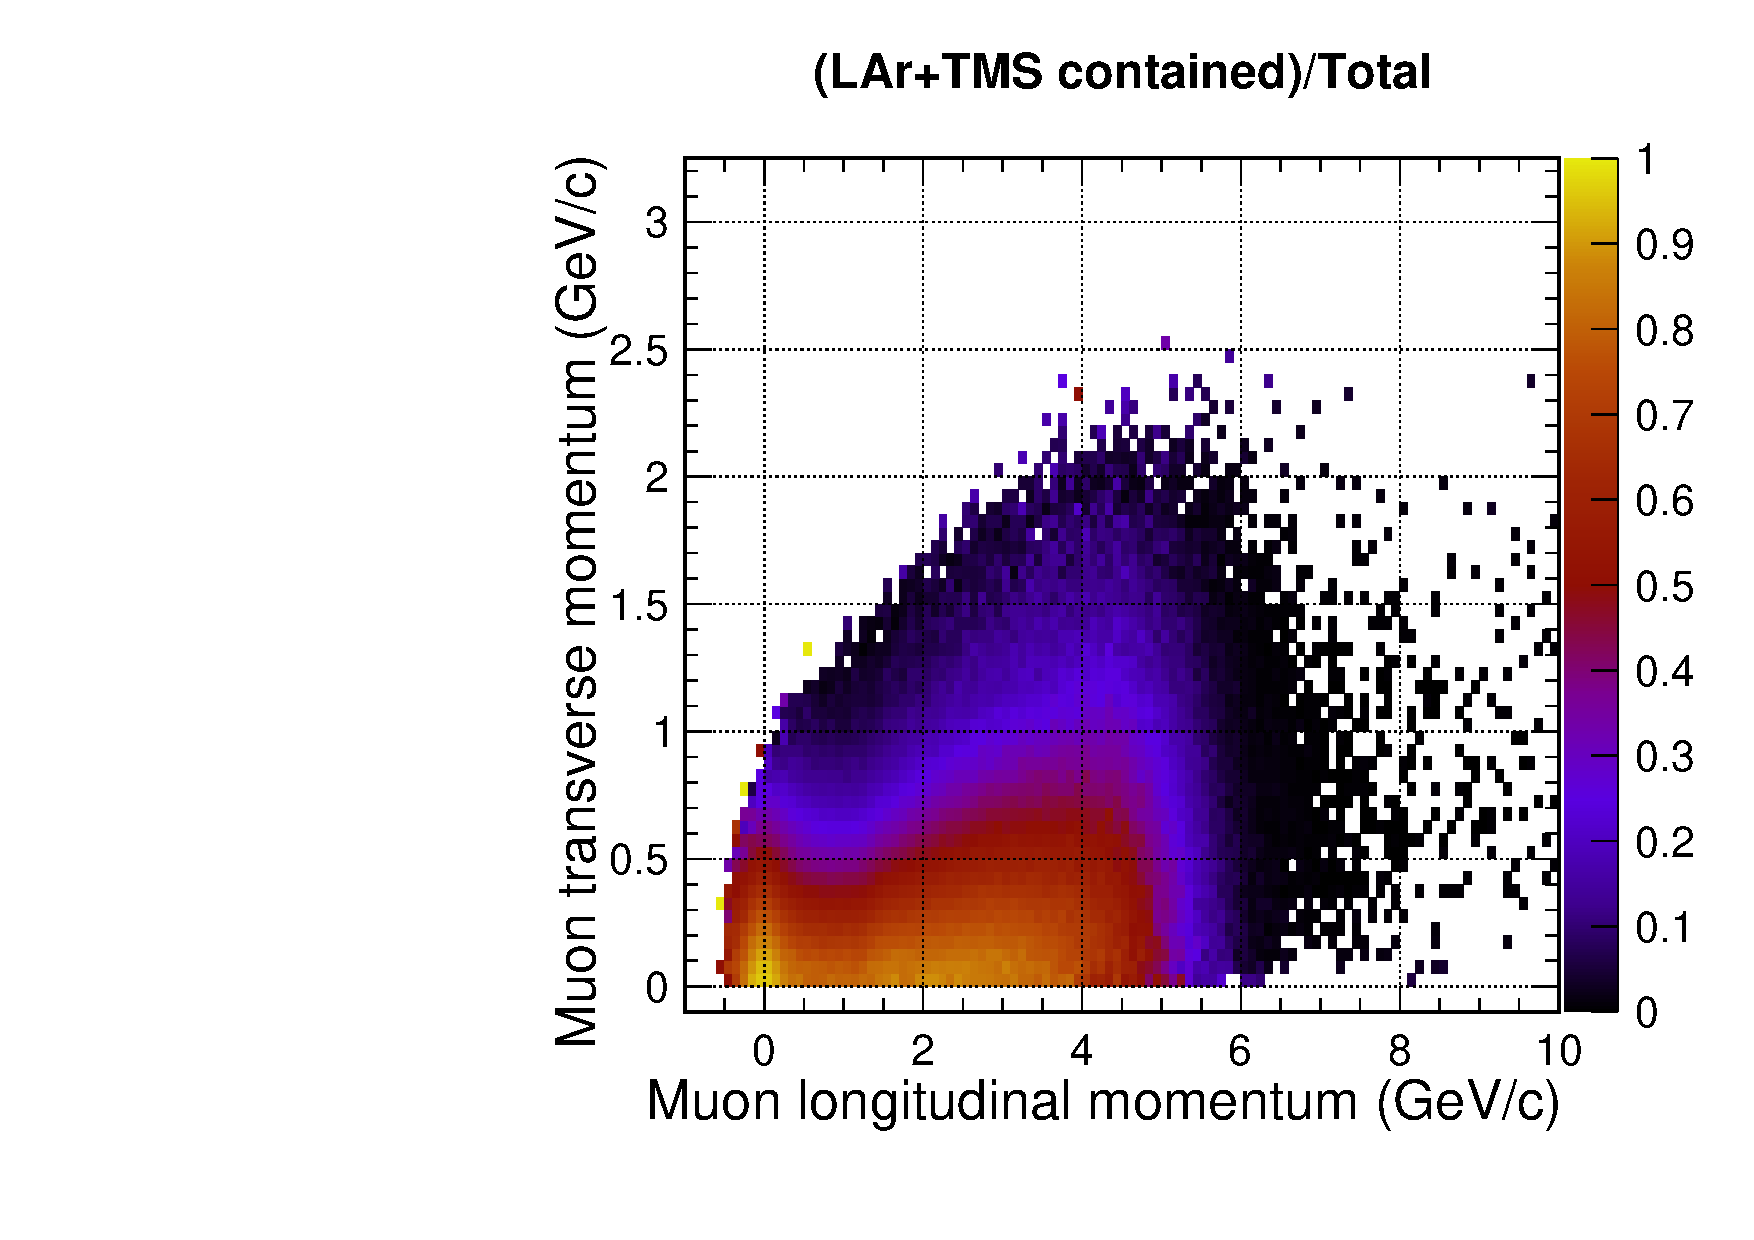
\includegraphics[width=0.5\textwidth]{graphics/tms/Simulation/LArTMSeff_muonptpl.pdf} 
\end{dunefigure}

In Figure \ref{fig:eff_enu_th20} we repeat the acceptance study in $E_\nu$, but include a $\theta_{\nu,\mu}<20\degree$ cut to better characterize \dword{ndlar}+\dword{tms} acceptance with events that dominantly are contained only by TMS. We see the \dword{ndlar} acceptance drop more aggressively with increasing neutrino energy with the $\theta_{\nu,\mu}$ cut, reaching 10\% at $E_\nu\sim 1.5\text{ GeV}$. However, the \dword{tms} acceptance rises at a similar rate, peaking at $E_\nu\sim1.9\text{ GeV}$ with 55\% acceptance. The overall acceptance drops below 50\% when $E_\nu>4.5\text{ GeV}$.
% Overall acceptance in neutrino energy
\begin{dunefigure}[Acceptance as a function of neutrino energy with muon angle cut]{fig:eff_enu_th20}
{Acceptance of the \dword{ndlar}, \dword{tms} and combined system in $E_\nu^\text{True}$ with $\theta_{\nu,\mu}<20\degree$. Left shows the events starting in the \dword{ndlar} and contained in the different detectors, compared with all events. Right shows the ratio of each category relative the total.}
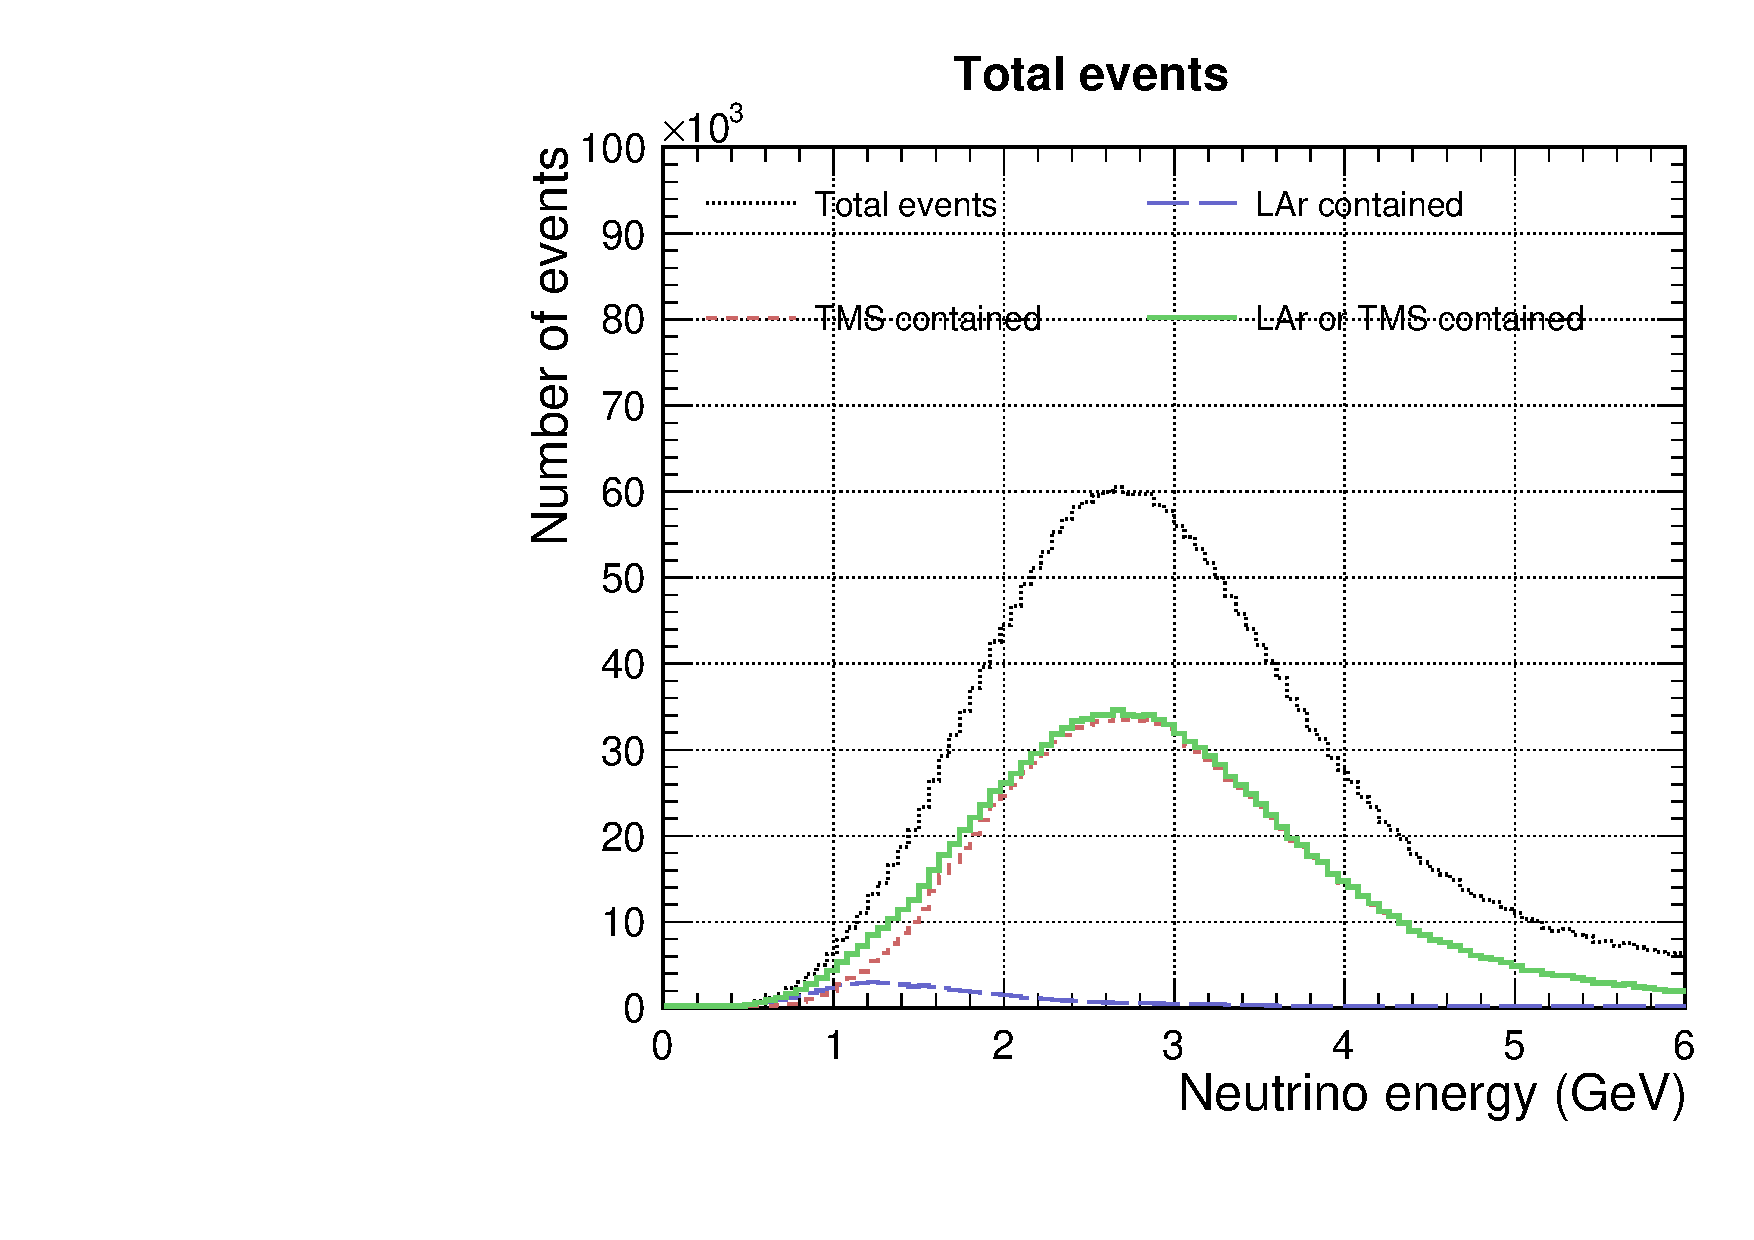
\includegraphics[width=0.49\textwidth, clip, trim={0mm 0mm 0mm 10mm}]{graphics/tms/Simulation/Efficiency/eff_20deg.pdf} 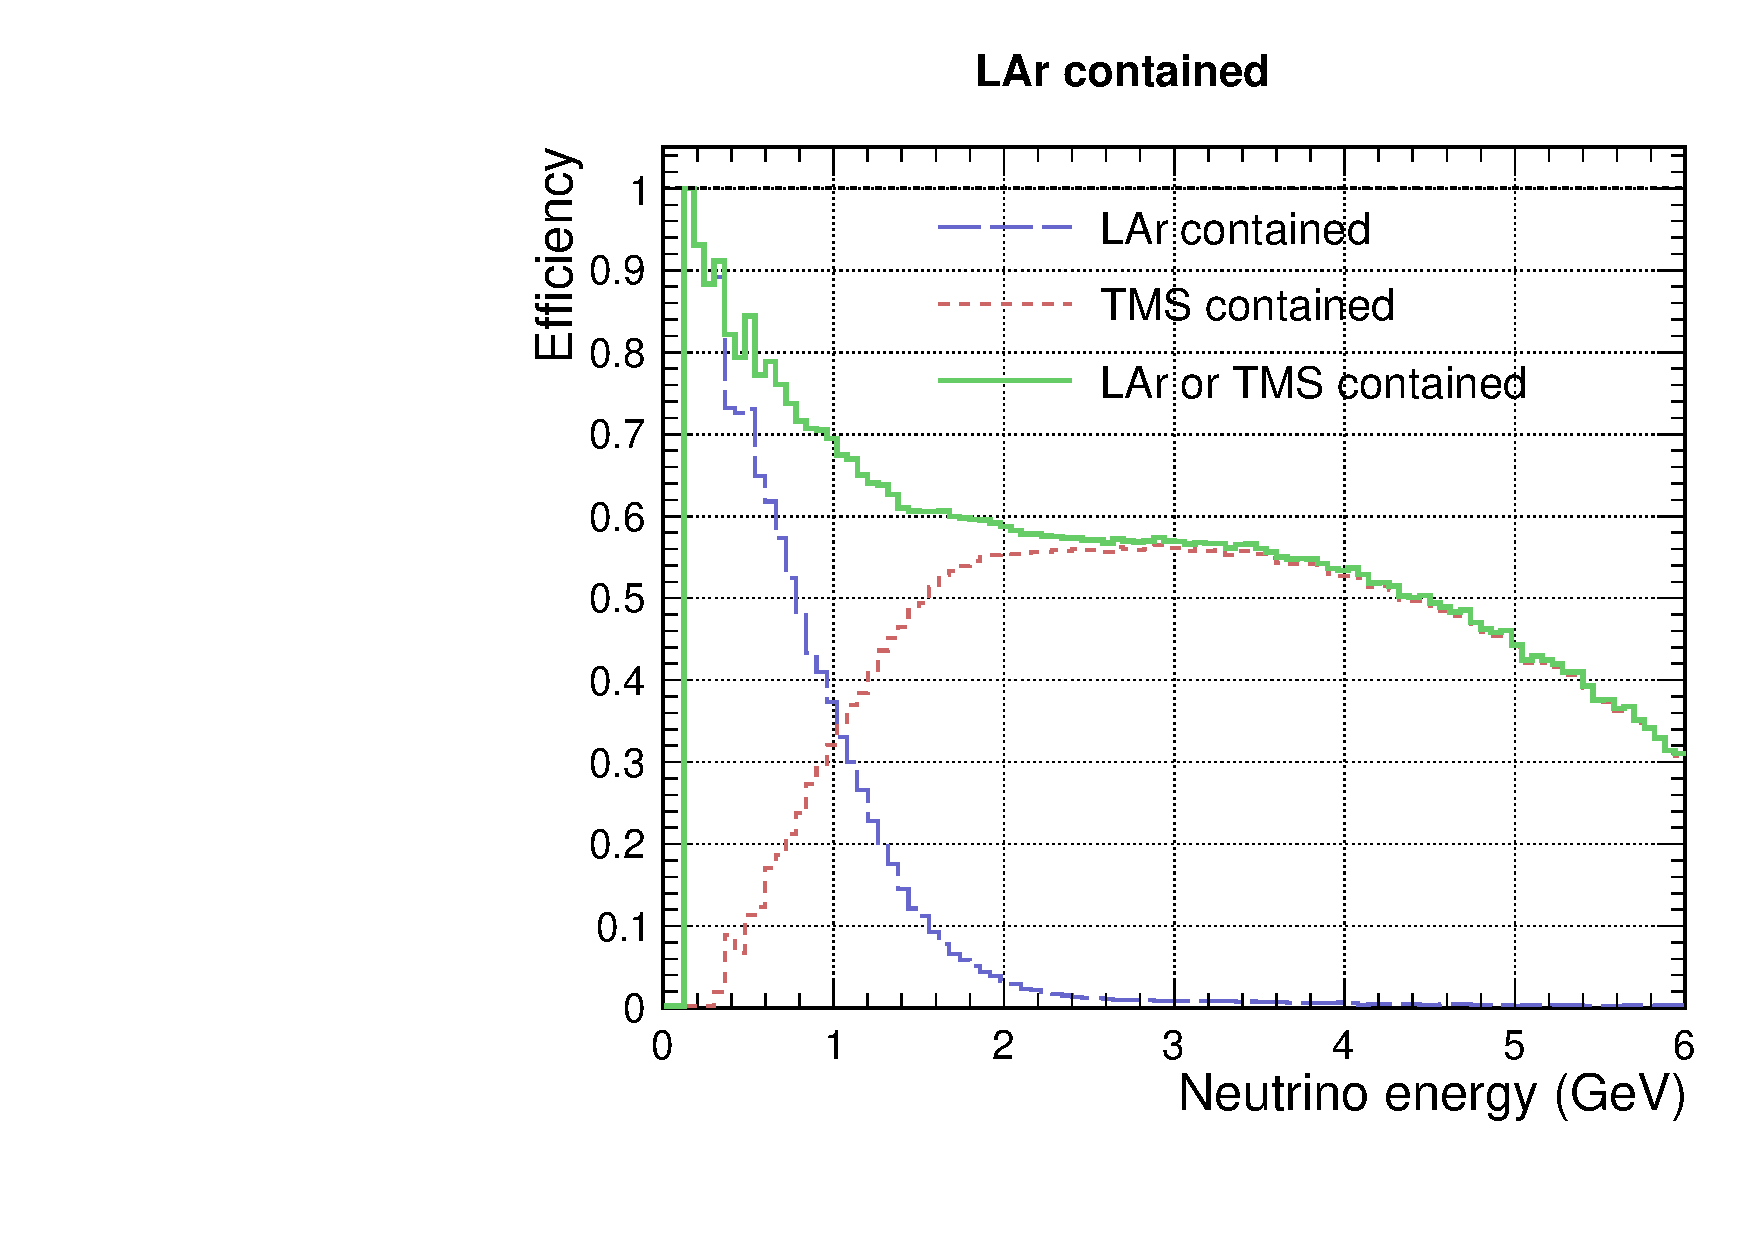
\includegraphics[width=0.49\textwidth, clip, trim={0mm 0mm 0mm 10mm}]{graphics/tms/Simulation/Efficiency/eff_ratio_20deg.pdf}
\end{dunefigure}

Figure \ref{fig:eff_ke} shows the acceptance in $T_\mu$, the muon kinetic energy after the neutrino interaction in the \dword{ndlar}, without any angular cuts.   The \dword{ndlar} contained events drop rapidly as the total events reaches its peak at 500 MeV. The \dword{tms} acceptance is low at low kinetic energies, mostly due to the muons not making it into the \dword{tms} and this acceptance including all $\theta_{\nu,\mu}$. The \dword{ndlar}+\dword{tms} acceptance is dominated by the \dword{tms} above $T_\mu=1\text{ GeV}$, and rises to 50\% at 3 GeV. 
% Overall acceptance in LAr KE
\begin{dunefigure}[Acceptance as a function of muon kinetic energy]{fig:eff_ke}
{Acceptance of the \dword{ndlar}, \dword{tms} and combined system in $T_\mu$ in the \dword{ndlar}. Left shows the events starting in the \dword{ndlar} and contained in the different detectors, compared with all events. Right shows the ratio of each category relative the total.}
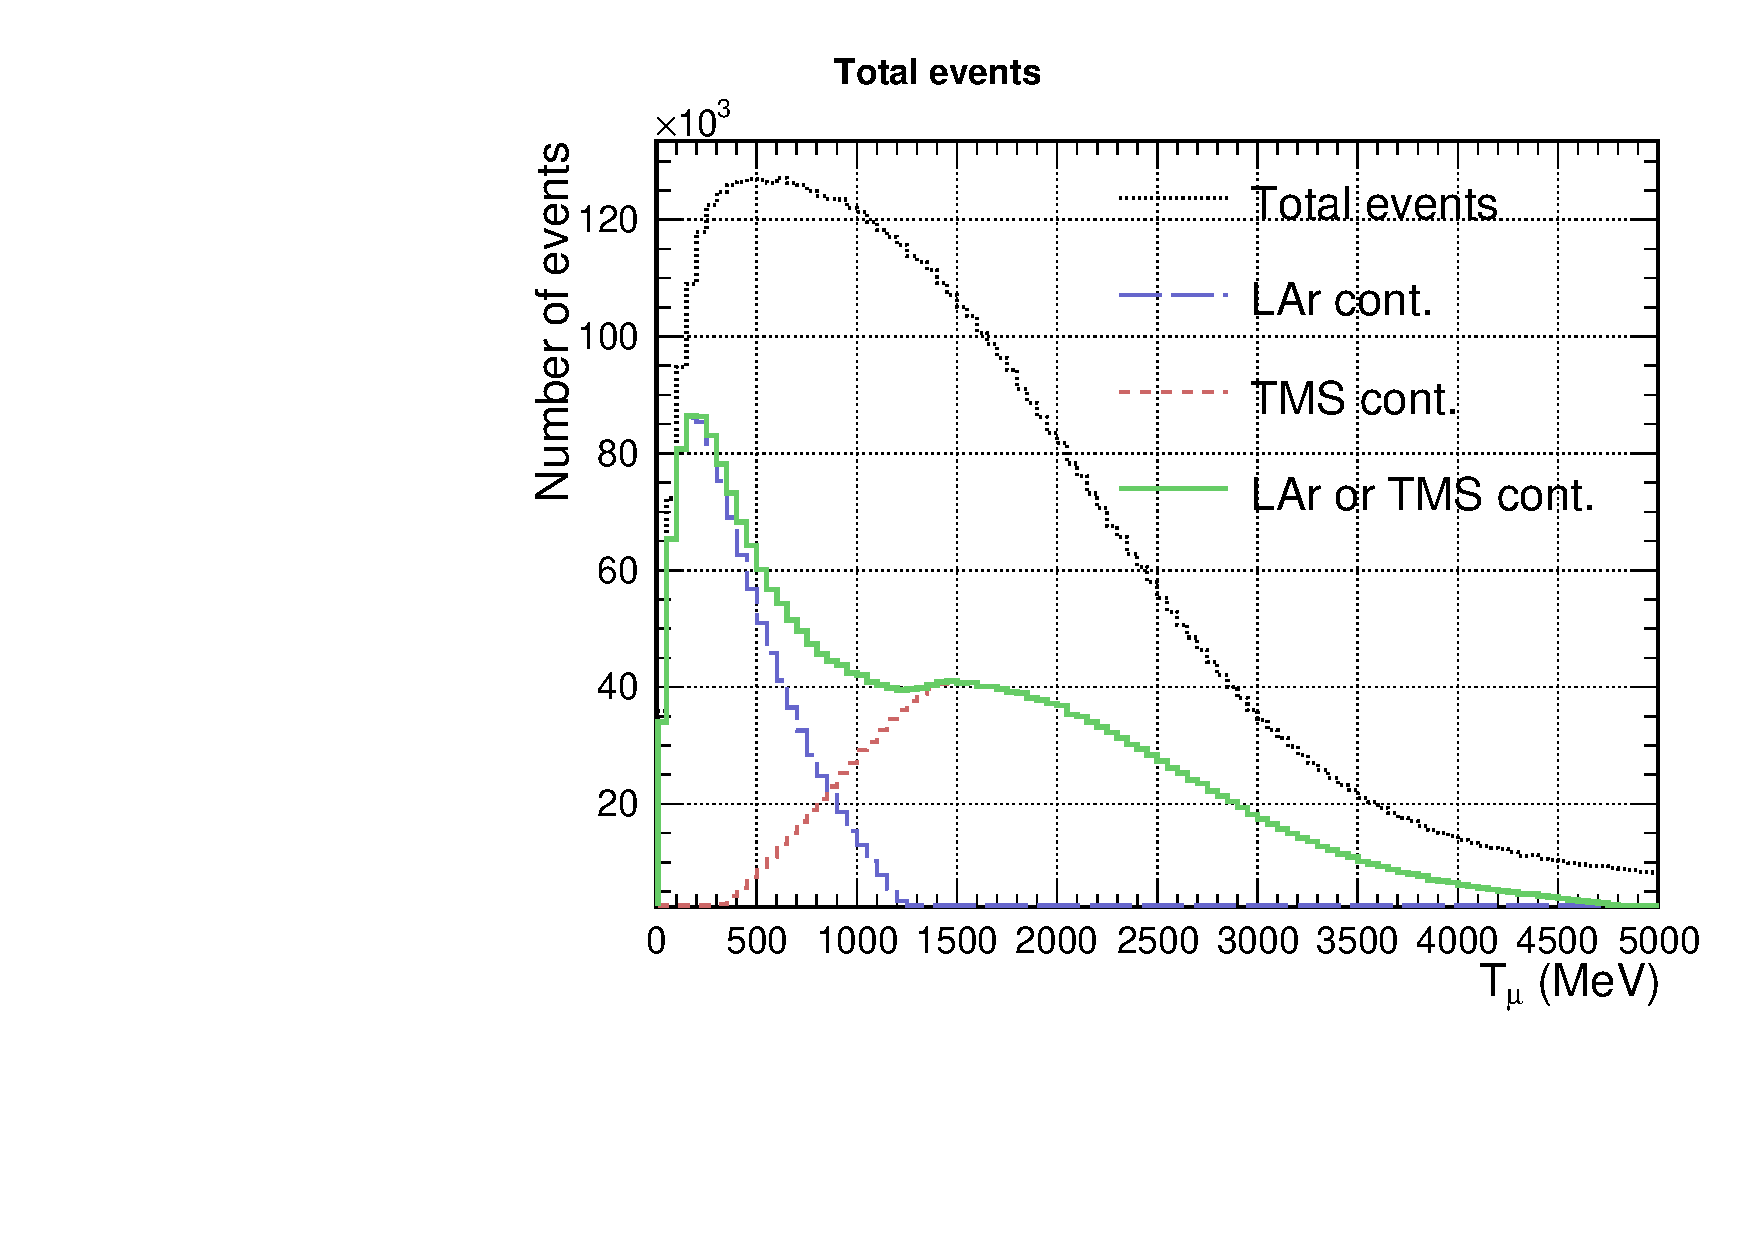
\includegraphics[width=0.49\textwidth, clip, trim={0mm 0mm 0mm 10mm}]{graphics/tms/Simulation/Efficiency/eff_muke.pdf} 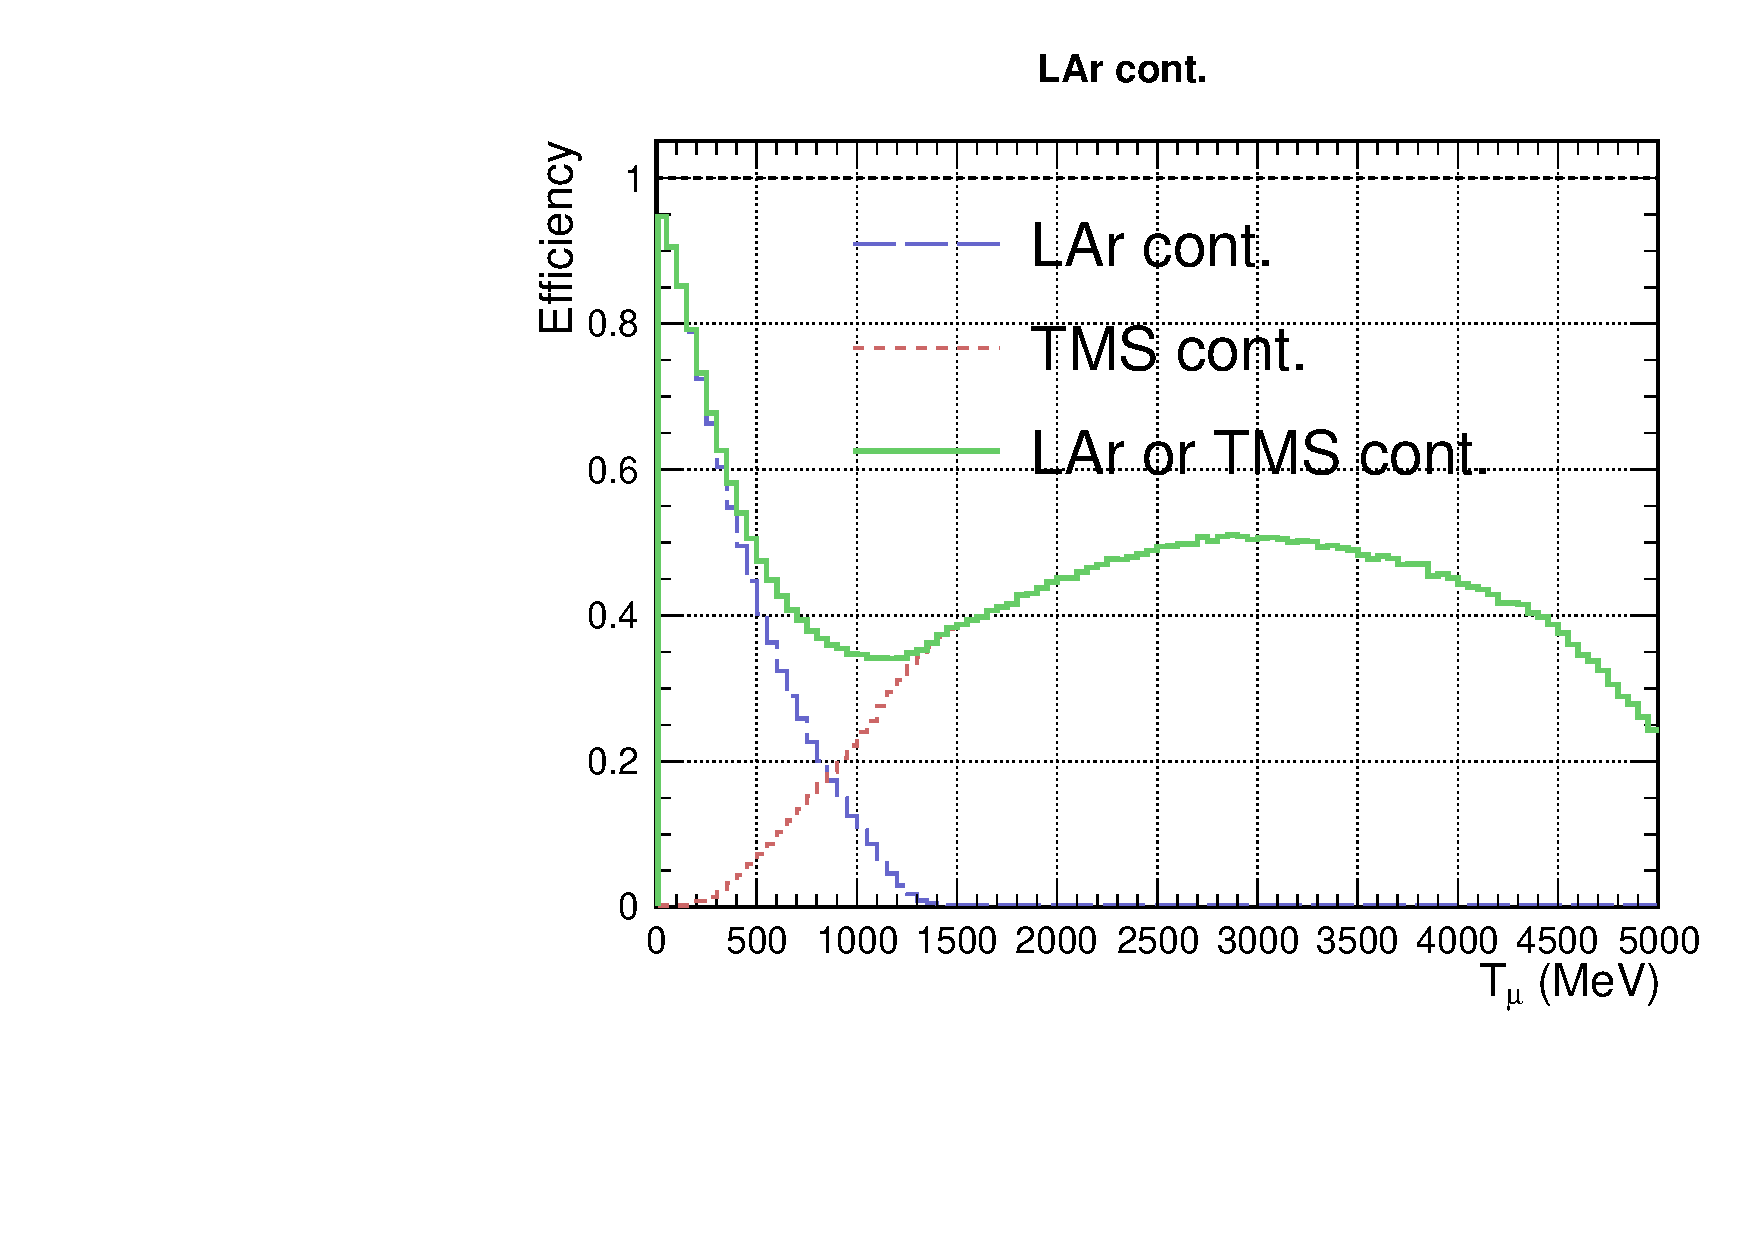
\includegraphics[width=0.49\textwidth, clip, trim={0mm 0mm 0mm 10mm}]{graphics/tms/Simulation/Efficiency/eff_muke_ratio.pdf}
\end{dunefigure}

In Figure \ref{fig:eff_ke_20deg} we additionally include the $\theta_{\nu,\mu}<20\degree$ cut and look at the acceptance in $T_\mu$. The total event distribution shifts considerably to higher energy, now peaking at 2 GeV. The \dword{tms} captures the event distribution peak very well, with a flat acceptance of 55\% when $1 < T_\mu < 3 \text{ GeV}$.
% th_mu_nu < 20 deg acceptance in LAr KE
\begin{dunefigure}[Acceptance as a function of muon kinetic energy with muon angle cuts]{fig:eff_ke_20deg}
{Efficiency of the \dword{ndlar}, \dword{tms} and combined system in $T_\mu$ in the \dword{ndlar} with $\theta_{\nu,\mu}<20\degree$. Left shows the events contained in the different detectors, compared with all events. Right shows the ratio of each category relative the total.}
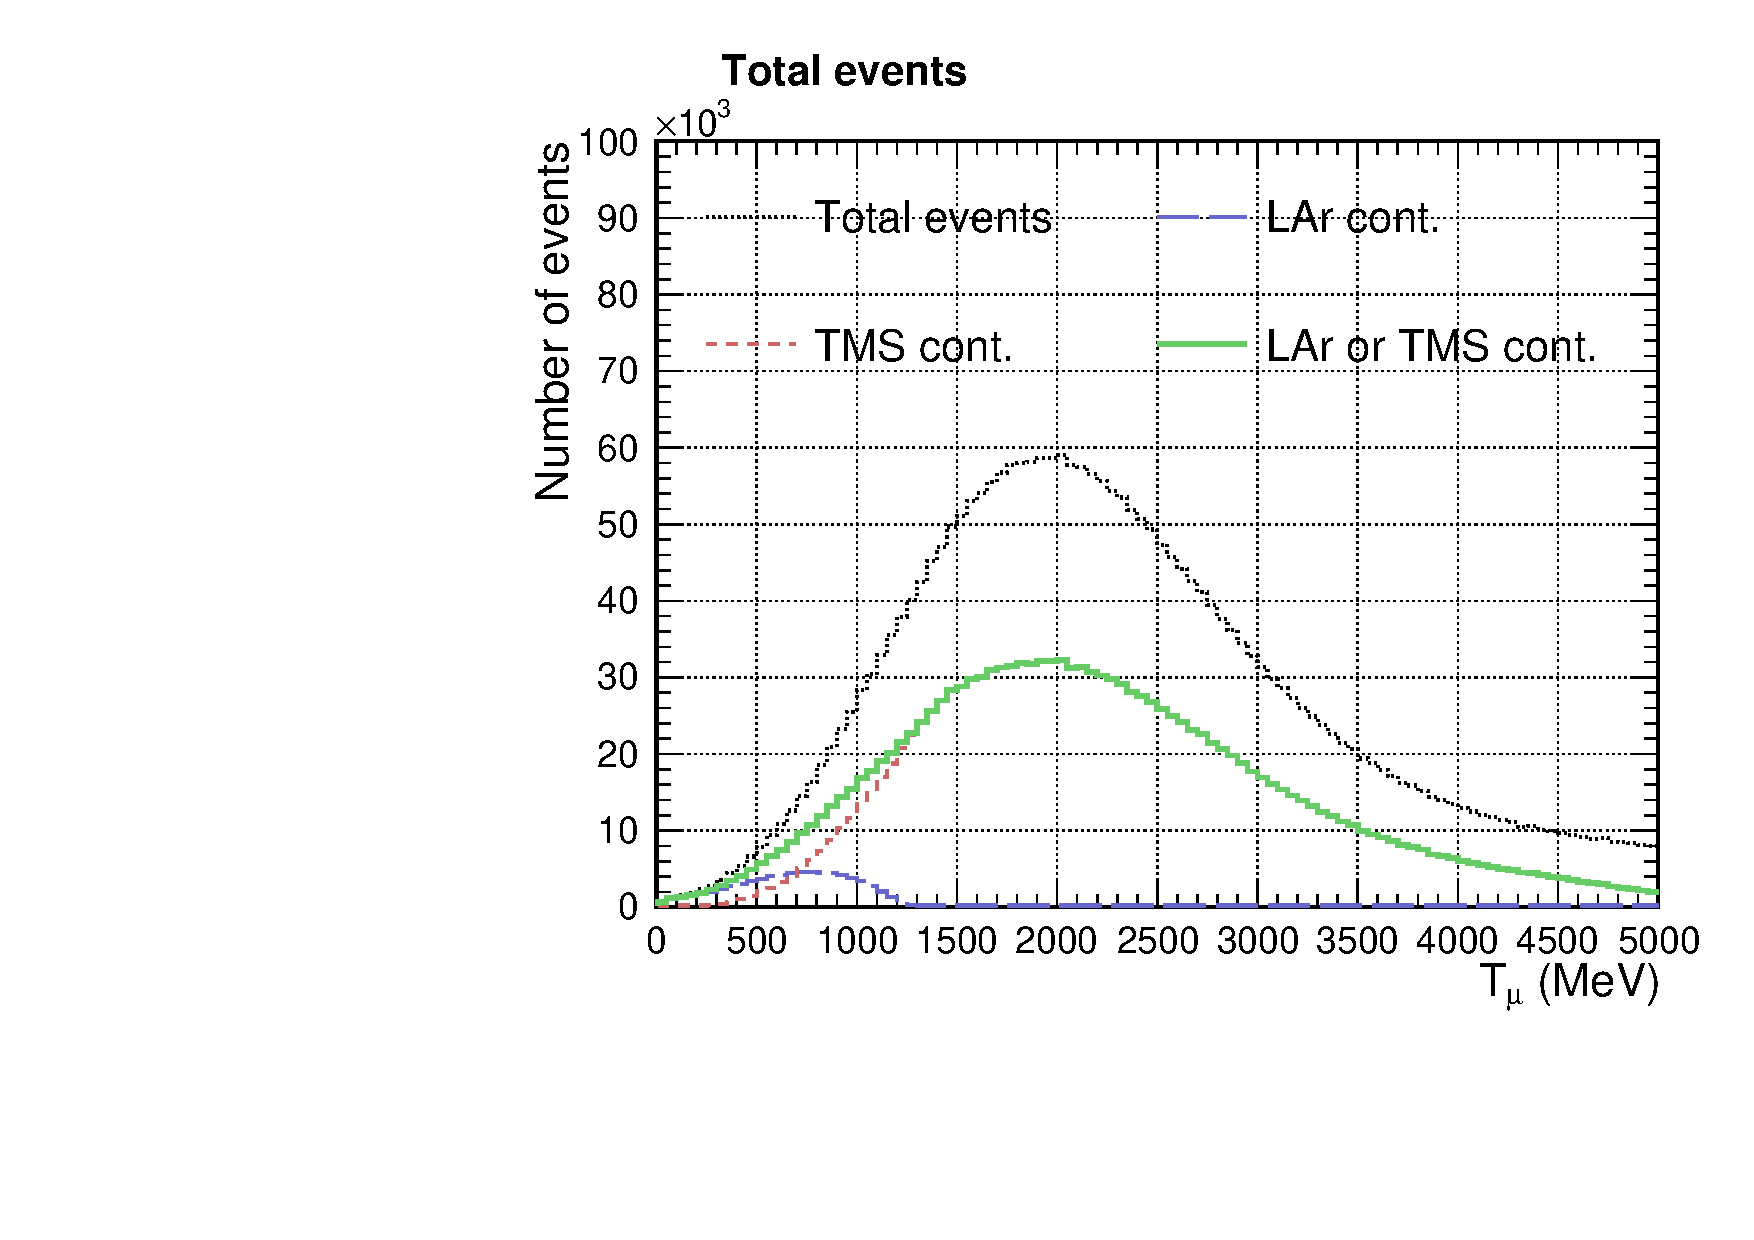
\includegraphics[width=0.49\textwidth, clip, trim={0mm 0mm 0mm 10mm}]{graphics/tms/Simulation/Efficiency/eff_muke_th20.pdf} 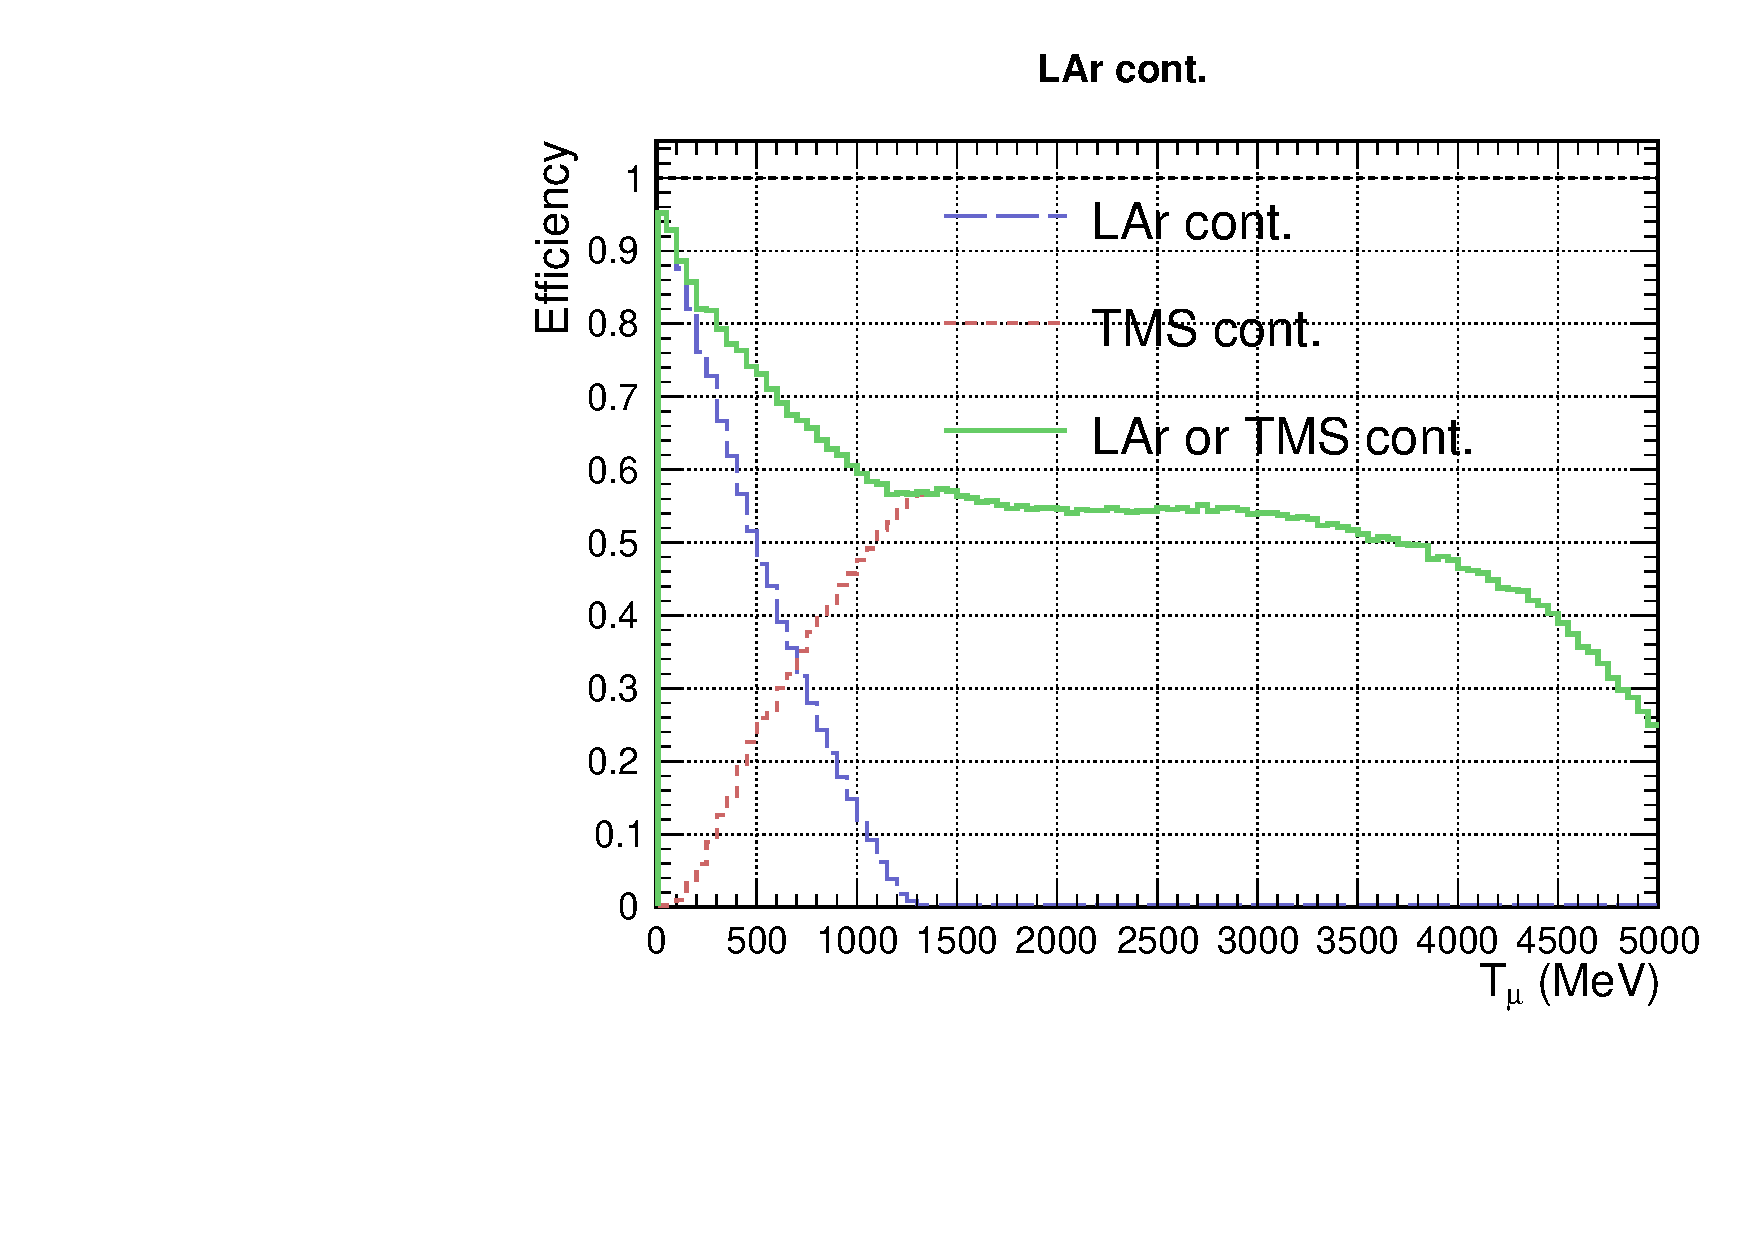
\includegraphics[width=0.49\textwidth, clip, trim={0mm 0mm 0mm 10mm}]{graphics/tms/Simulation/Efficiency/eff_muke_th20_ratio.pdf}
\end{dunefigure}

\subsubsection{Muon Momentum Resolution}
\label{sec:muonres}
Particle trajectories in the \dword{tms} differ from a traditional magnetic spectrometer. In the \dword{tms}, a track's sagitta is, apart from energy loss, independent of momentum: the bend of a track per unit length is inversely proportional to momentum, but its range is proportional. The momentum measurement from the magnetic field is driven not by the magnitude of the sagitta, but by where the sagitta occurs longitudinally. Consequently, we determine the momentum of the muon via its range which is more sensitive in the kinematic regime we operate in, rather than by its curvature. The reconstruction that is being developed will however include both effects in fitting the muon track.

Figure \ref{fig:TrackLength_KE} shows the density-weighted track length of the primary muon ($x\rho$, where $x$ is the track length and $\rho$ is the density) against the muon's kinetic energy at the vertex in the \dword{ndlar}. The resulting relationship is very linear as expected, with the slope and intercept agreeing with expectation of the iron and scintillator structure of the \dword{tms}. The small population at low track length for all muon kinetic energy are from tracks with a large fraction of their trajectory in the 7 cm central gap region, which has no scintillator instrumented. We also show the Monte-Carlo estimate of the smearing between the true muon kinetic energy at the \dword{ndlar} vertex to the true muon kinetic energy at the \dword{tms} entrance point. Mapping one to the other requires some understanding of the energy loss in the \dword{ndlar} and in the gap region between the \dword{ndlar} and \dword{tms} detectors; here we have assumed a straight-line track length of 24.35 $g/cm^{2}$ between the detectors, which is then corrected to account for the angle subtended by the muon \dword{ndlar} exit and \dword{tms} entrance points. 

\begin{dunefigure}[True kinetic energy of the muon versus track length]{fig:TrackLength_KE}
{True kinetic energy of the muon at the LAr vertex versus track length (left) and the relationship between the muon kinetic energy at the vertex in the \dword{ndlar} and the entrance kinetic energy in the \dword{tms} (right).}
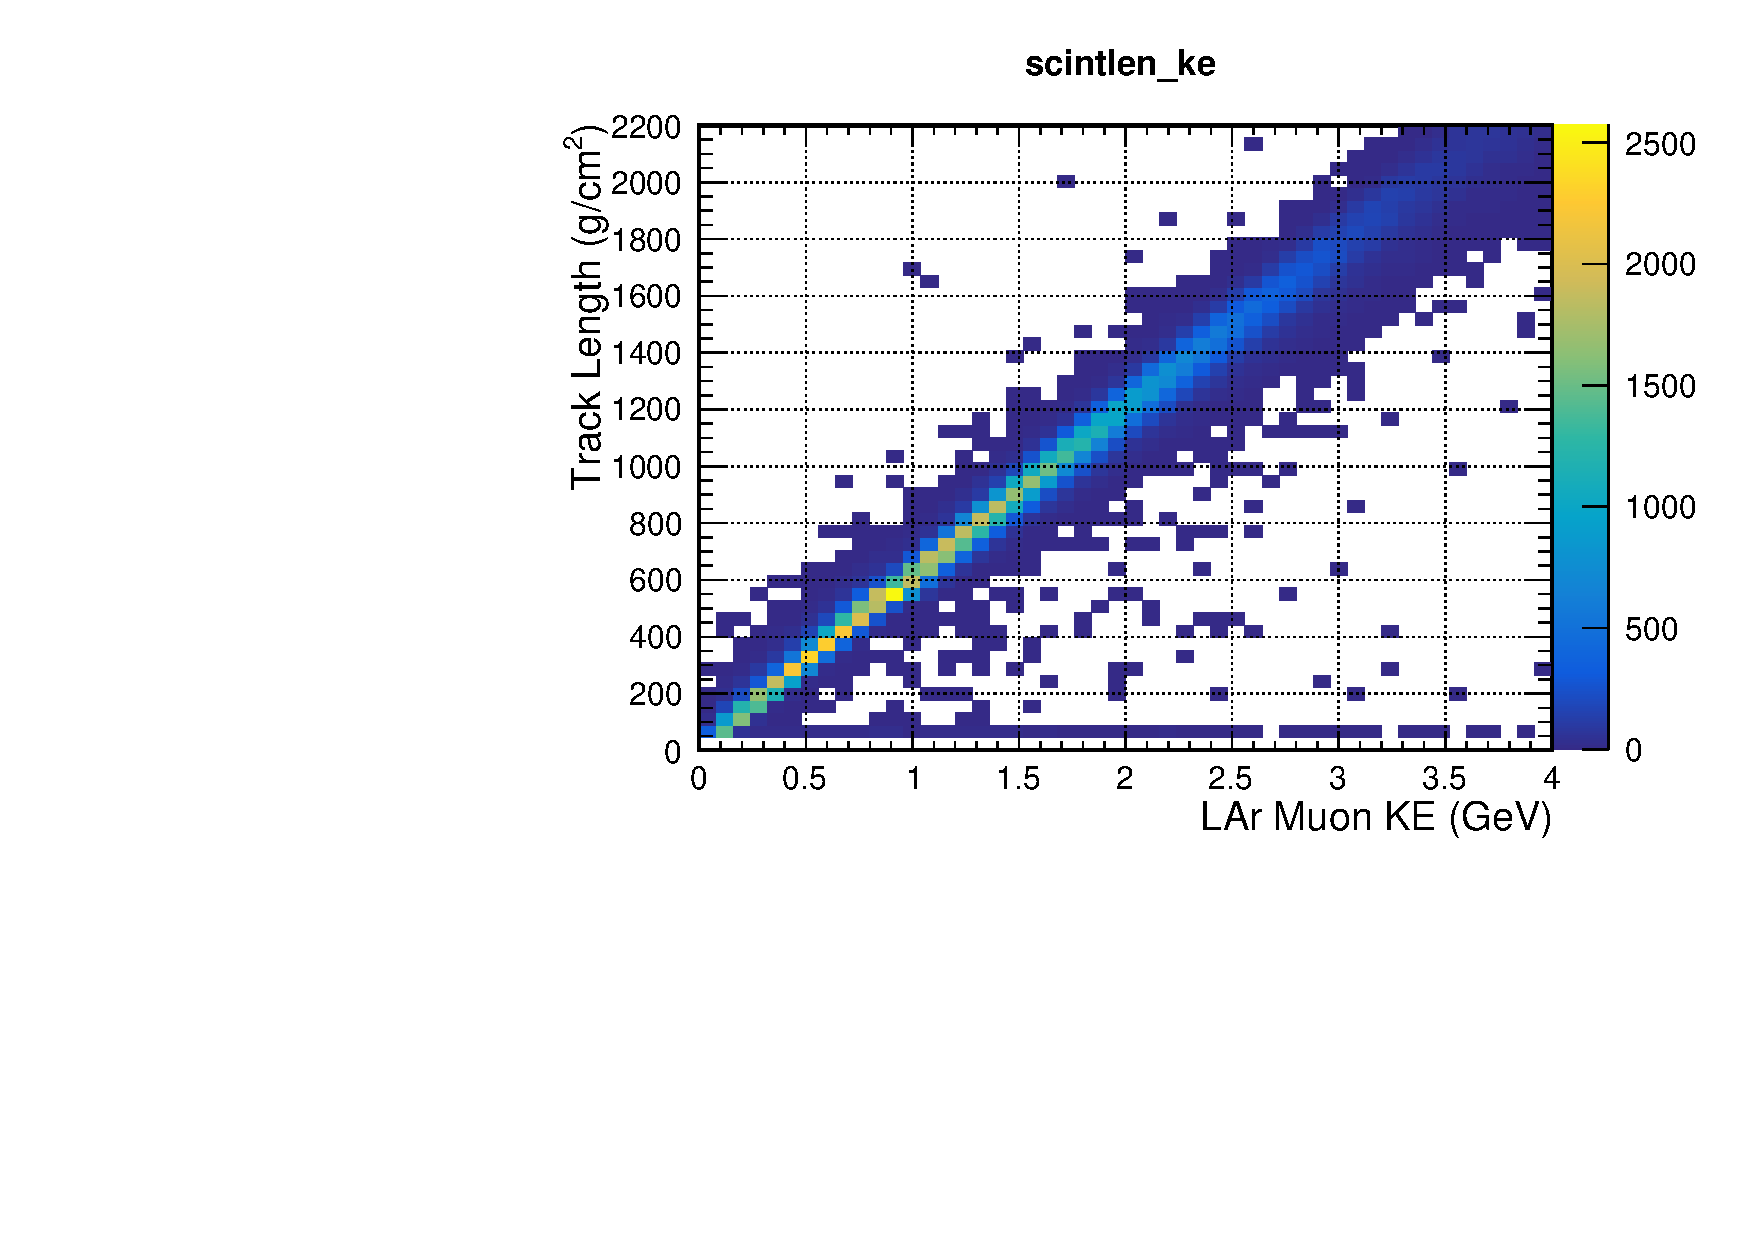
\includegraphics[width=0.49\textwidth, clip, trim={0mm 0mm 0mm 10mm}]{graphics/tms/Simulation/KE_est/track_length_LArKE.pdf}
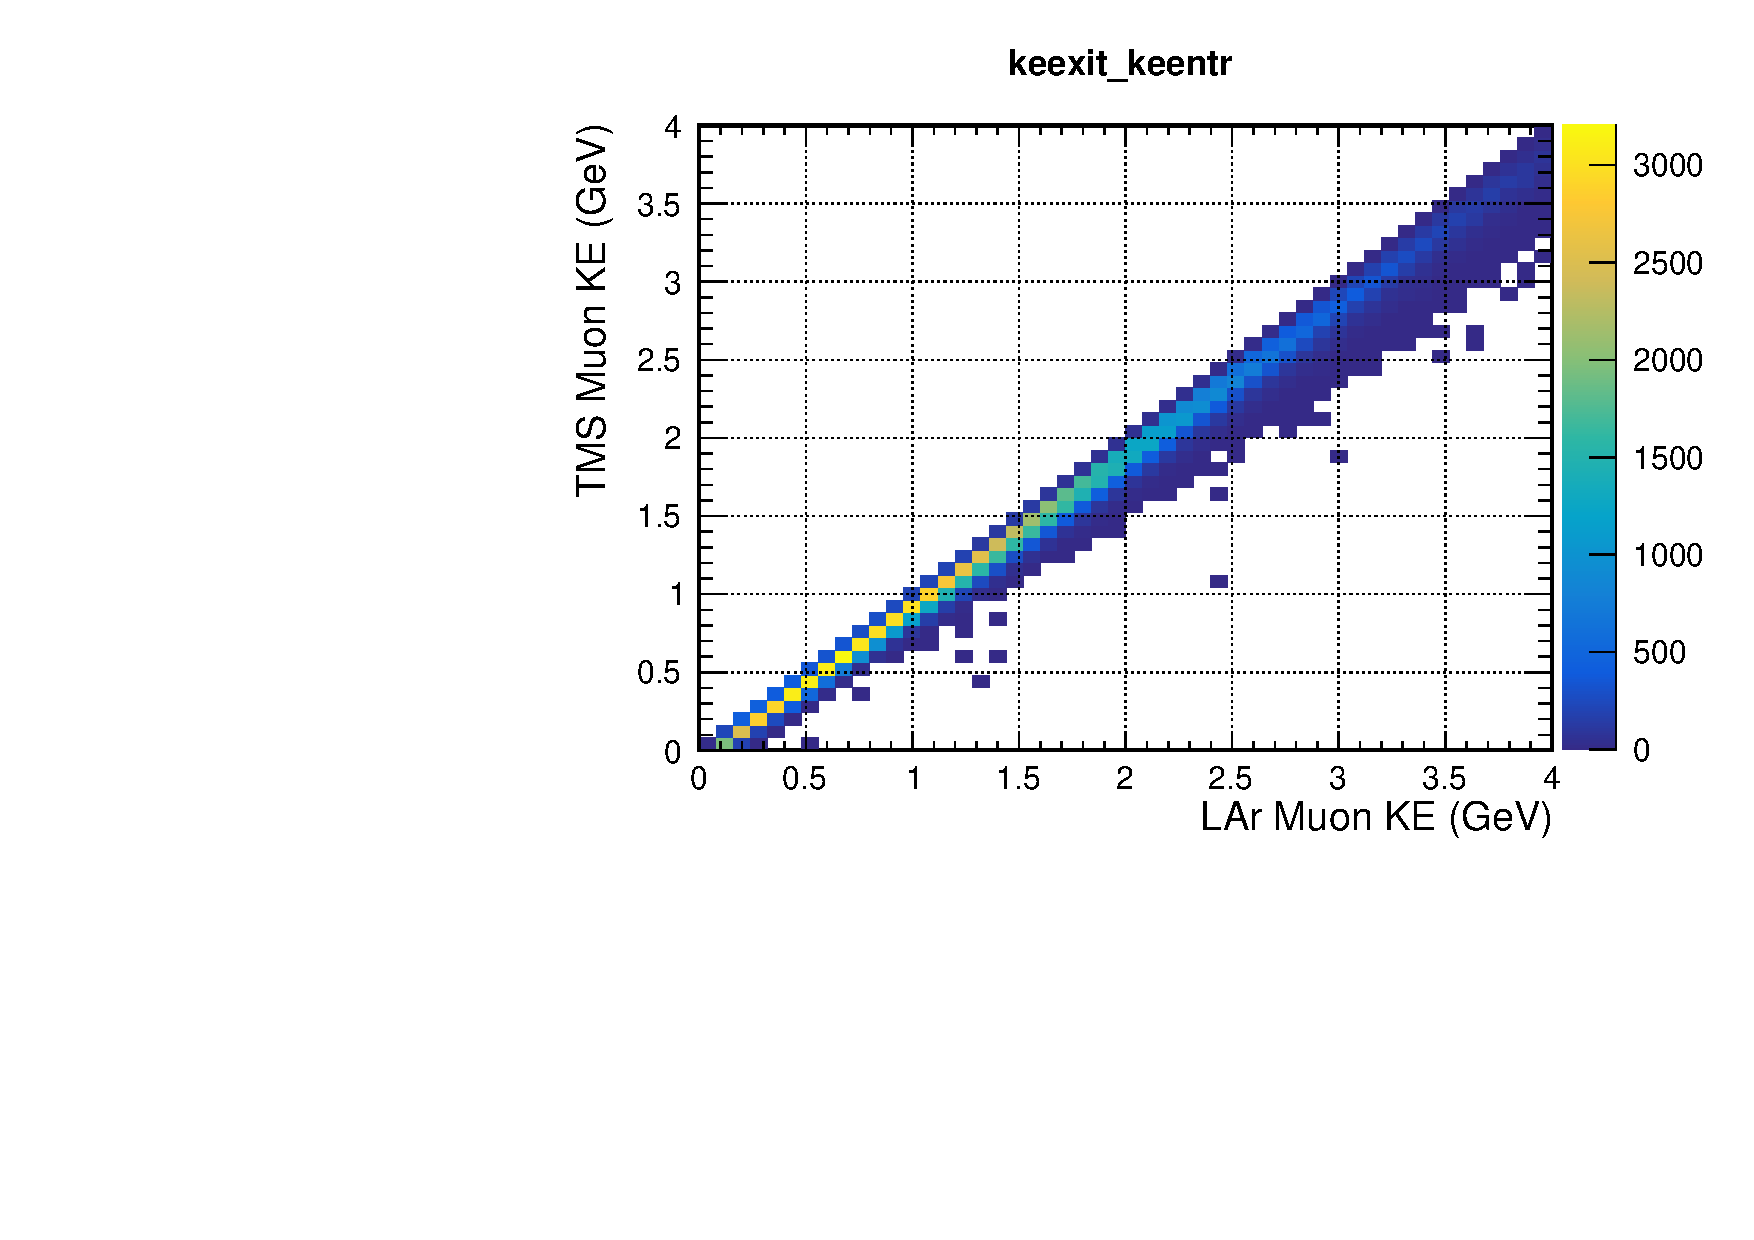
\includegraphics[width=0.49\textwidth, clip, trim={0mm 0mm 0mm 10mm}]{graphics/tms/Simulation/KE_est/LArKE_TMSKE.pdf}
\end{dunefigure}

In Figure \ref{fig:LAr_TMS_KE} we show the simple linear estimator between the muon kinetic energy in the \dword{ndlar} and its estimator from using only the track length from Figure \ref{fig:TrackLength_KE}. The relationship clearly follows that of Figure \ref{fig:TrackLength_KE}. On the right, we show the relationship between the bias of the KE estimator based on track length and the total deposited scintillation energy along the track. This figure implies that a measure of a track's energy deposits could be used to better reconstruct the muon kinetic energy than track length alone. We calculate the resoluton and bias by fitting a Gaussian distribution to each slice of true muon KE against the reconstructed muon KE using track length. This simple estimator has $6-8\%$ resolution for muons with KE above 1 GeV at the LAr vertex, with a bias between -1--2\%, improving with increased kinetic energy, 
\begin{dunefigure}[Muon KE estimator from track length against the true muon KE]{fig:LAr_TMS_KE}
{The simple muon KE estimator from track length against the true muon KE at the \dword{ndlar} vertex (left). The bias in the KE estimator against the total deposited energy for a track (right).}
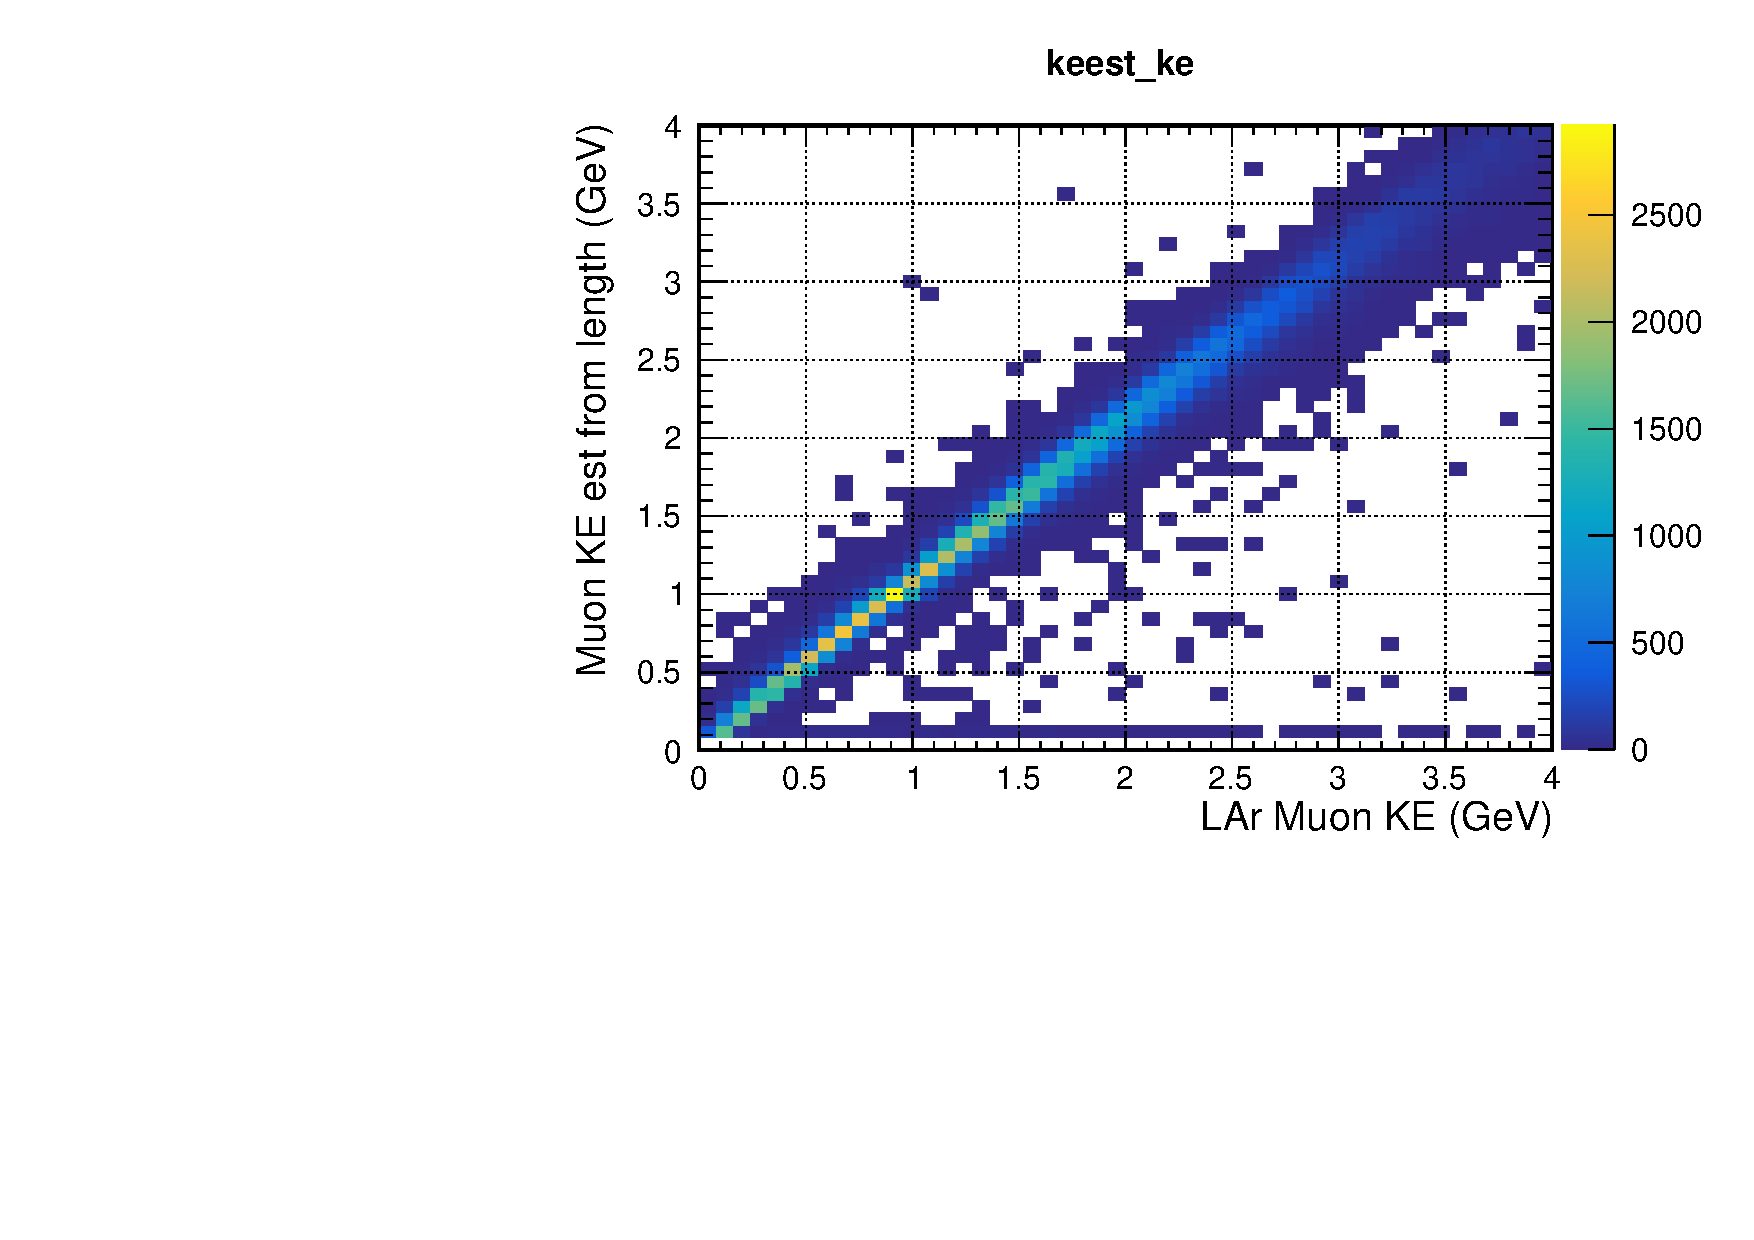
\includegraphics[width=0.49\textwidth, clip, trim={0mm 0mm 0mm 10mm}]{graphics/tms/Simulation/KE_est/muonKEest_muonKE.pdf}
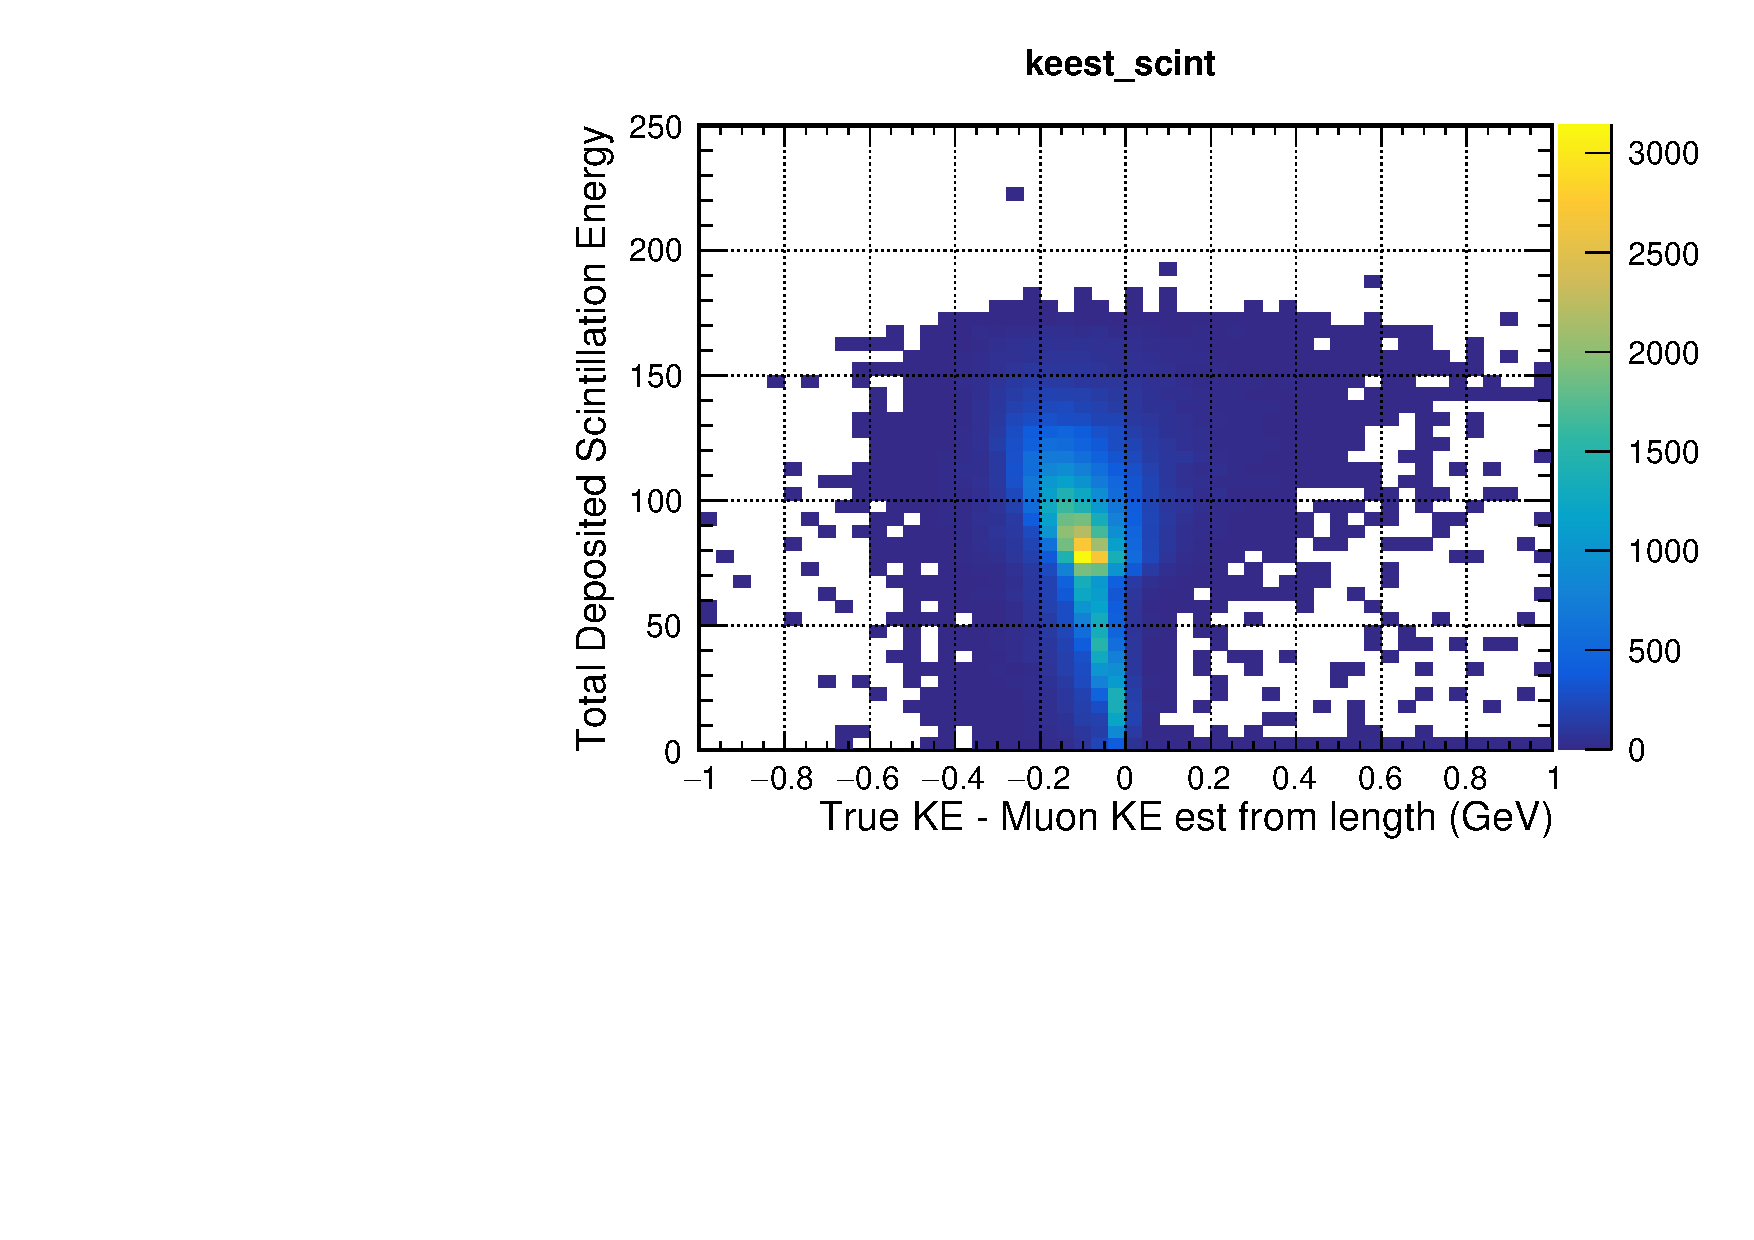
\includegraphics[width=0.49\textwidth, clip, trim={0mm 0mm 0mm 10mm}]{graphics/tms/Simulation/KE_est/bias_energydeposit.pdf}
\end{dunefigure}

If we focus on reconstructing the muon KE as it enters the \dword{tms} rather than the \dword{ndlar} vertex KE, we observe comparable performance to the MINOS figures presented at the start of this chapter in Figure \ref{fig:minos_resolution}. These studies are presented in Figure \ref{fig:TMS_KE}, where we note a tighter distribution of track length for each muon KE bin (directly impacting the resolution), the distribution at low track length is gone, and a wider and higher distribution of muon kinetic energy. As before, the simple estimator of muon KE from density-weighted track length agrees well with expectation from the \dword{tms} composition. At 1 GeV we observe muon KE resolutions around 7\%, decreasing to about 5\% above 2 GeV. The bias is similar to when estimating the muon KE at the \dword{ndlar} vertex; approximately -1--2\%.
\begin{dunefigure}[True kinetic energy of the muon at the \dword{tms} entrance point versus track length]{fig:TMS_KE}
{True kinetic energy of the muon at the \dword{tms} entrance point versus track length (left). The simple muon KE estimator from track length against the true muon KE at the \dword{tms} entrance point (right).}
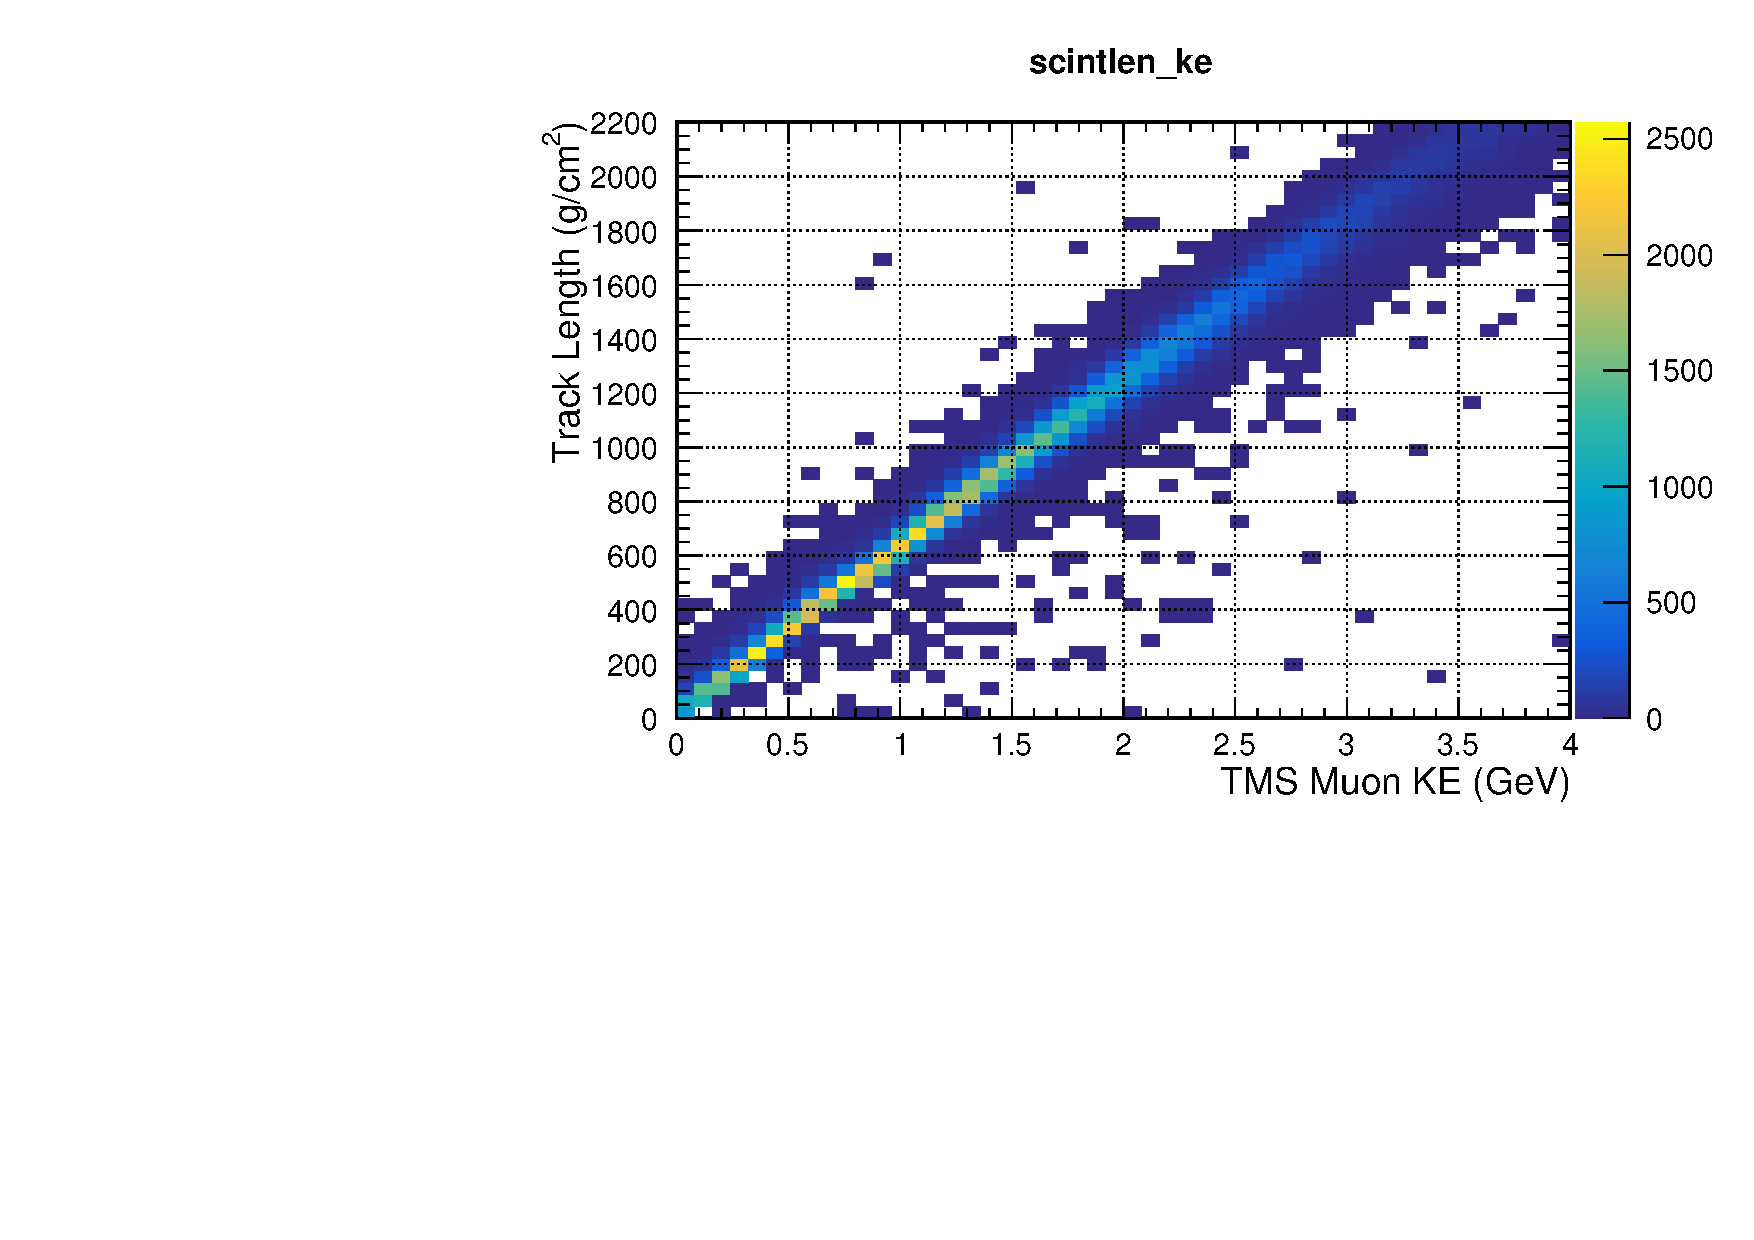
\includegraphics[width=0.49\textwidth, clip, trim={0mm 0mm 0mm 10mm}]{graphics/tms/Simulation/KE_est/TMSKE_tracklength.pdf}
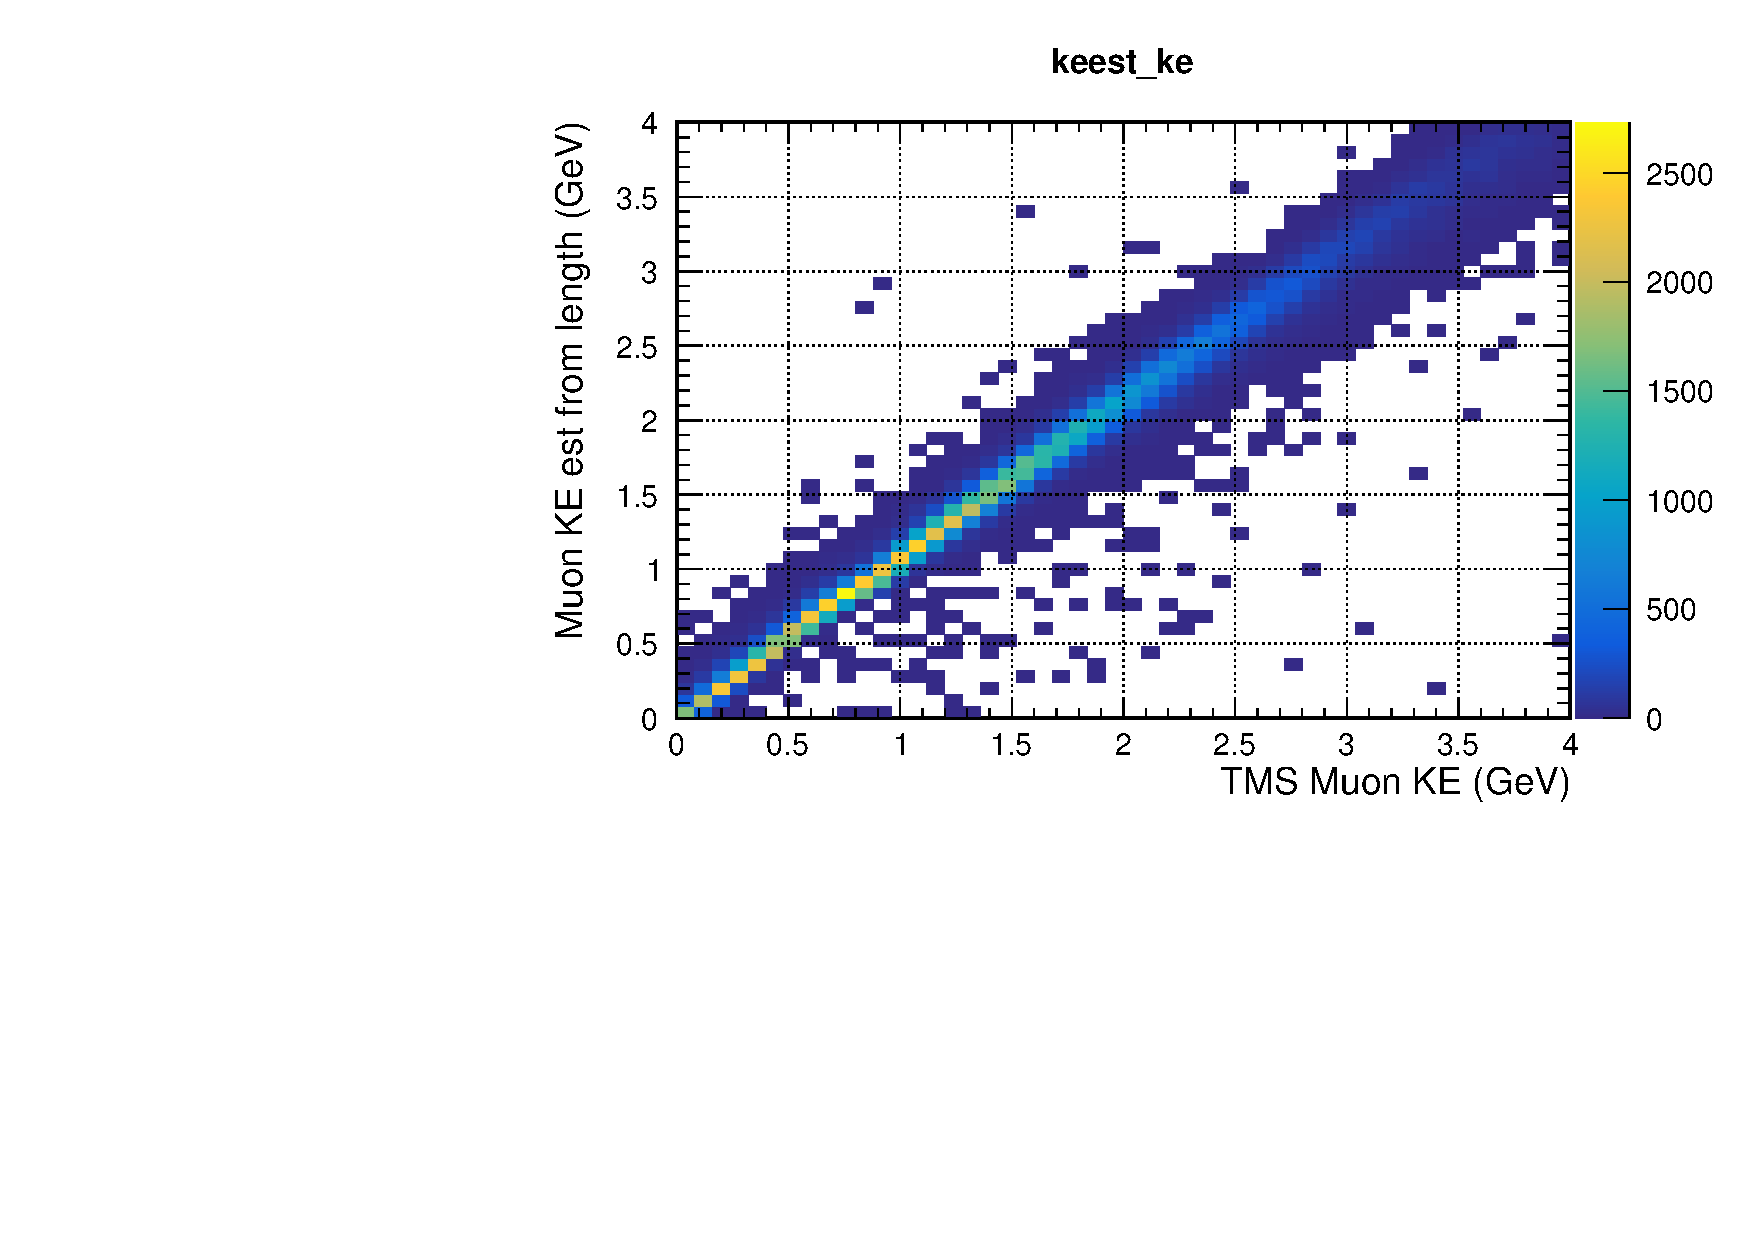
\includegraphics[width=0.49\textwidth, clip, trim={0mm 0mm 0mm 10mm}]{graphics/tms/Simulation/KE_est/TMSKE_est.pdf}
\end{dunefigure}

We stress that these resolution studies will increase in sophistication when the track fitter is finalised, using both the track length, energy deposits, and track bending to estimate the track momentum.

\subsubsection{Muon Sign Selection}
To study the bending of tracks in the \dword{tms} we use the $x-z$ view to look for deviations from a straight line. For events where the hits in the \dword{tms} fall within the central steel region, the method draws a straight line between the \dword{ndlar} start and endpoint, alternatively the \dword{ndlar} endpoint and the \dword{tms} start point, and projects it to the $z$ of the last hit of the track. This provides an estimate of the last hit position if it traversed in a straight line. If the last hit is above the the expected, the candidate is expected to have positive charge, and vice versa for negative charge. The procedure is outlined in Figure \ref{fig:bend_method}. 

As in previous section, we stress that the full reconstruction will \emph{not} use such a simple method, and will instead fit for particle charge in the track model. The choice of sign selection metric presented was chosen because it requires minimal reconstruction, so can be done early in the \dword{tms} design process to gauge performance.
\begin{dunefigure}[Method for calculating the ``signed distance'']{fig:bend_method}
{An example event display showing the method for calculating the ``signed distance'' metric (shown in yellow) for determining charge of the particle in the magnetic field in the truth studies.}
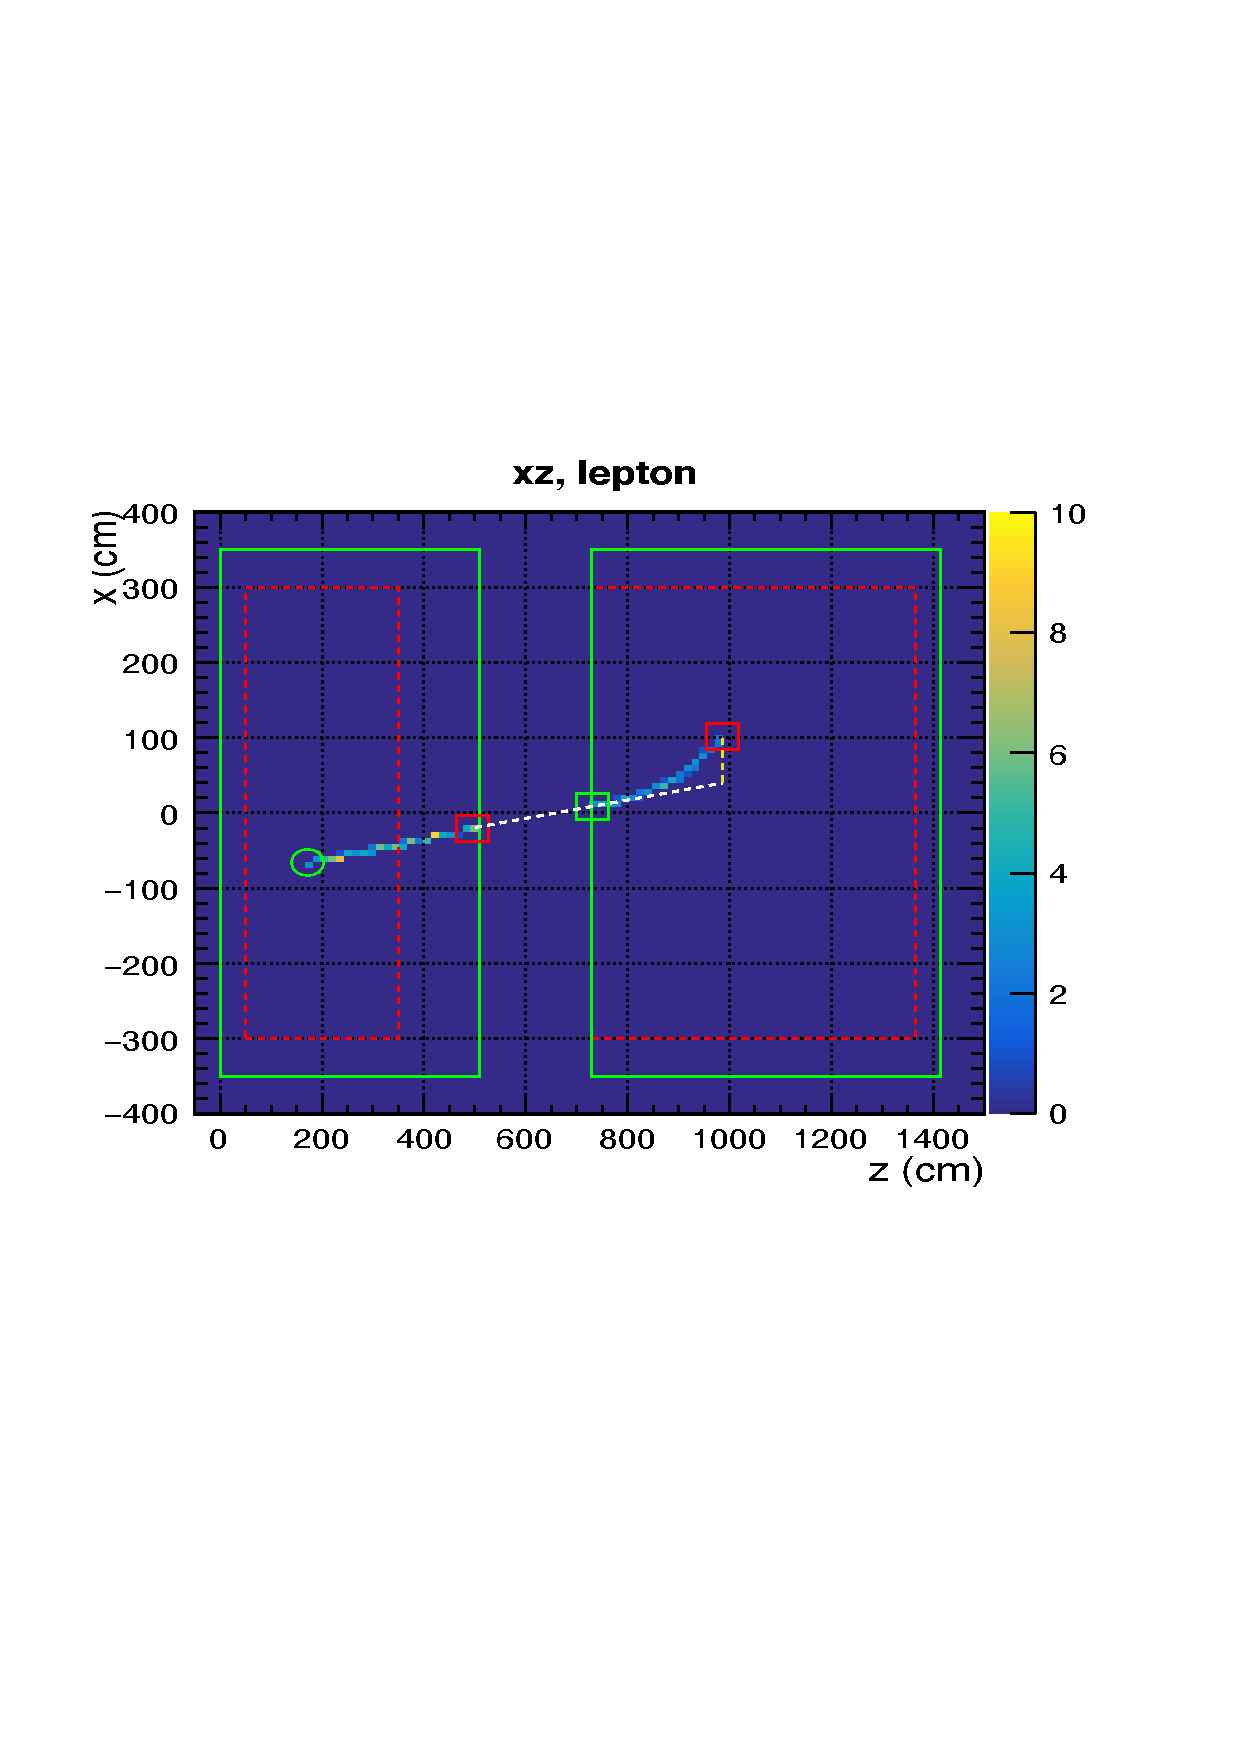
\includegraphics[width=0.6\textwidth, clip, trim={0mm 90mm 0mm 70mm}]{graphics/tms/Simulation/Bend/pg_0012_signed_dist.pdf}
\end{dunefigure}

The equation derived for the ``signed distance'' is
% Use Clarence's updated signed distance instead?
\begin{equation}
    %SD = \frac{(x_2-x_1) z_3 + x_1 z_2 - z_1 x_2 -(z_2-z_1)x_3}{\sqrt{(x_2-x_1)^2+(z_2-z_1)^2}}
    SD = (x_3-x_1) - (x_2-x_1)\frac{z_3-z_1}{z_2-z_1}
\end{equation}
where $x_{1,2,3},z_{1,2,3}$ is the $x,z$ position of the \dword{ndlar} exit point (or \dword{ndlar} start point), \dword{tms} entry point (or \dword{ndlar} exit point), and the last hit in the \dword{tms} respectively.

Figure \ref{fig:bend_results} shows the ``signed distance'' metric for the generated \dword{fhc} sample. This study only uses tracks in the center region to avoid the changing field in the left and right modules. The 3.5~cm counter quantization is not included in this study, but has only a minor impact over the bulk of the distribution.

\begin{dunefigure}[Determining the charge of the track from its bending]{fig:bend_results}
{The ``signed distance'' metric for determining the charge of the track from its bending. The success rate is tabulated in 
Table \ref{tab:muon_bend} for $\mu^-$ and $\mu^+$.}
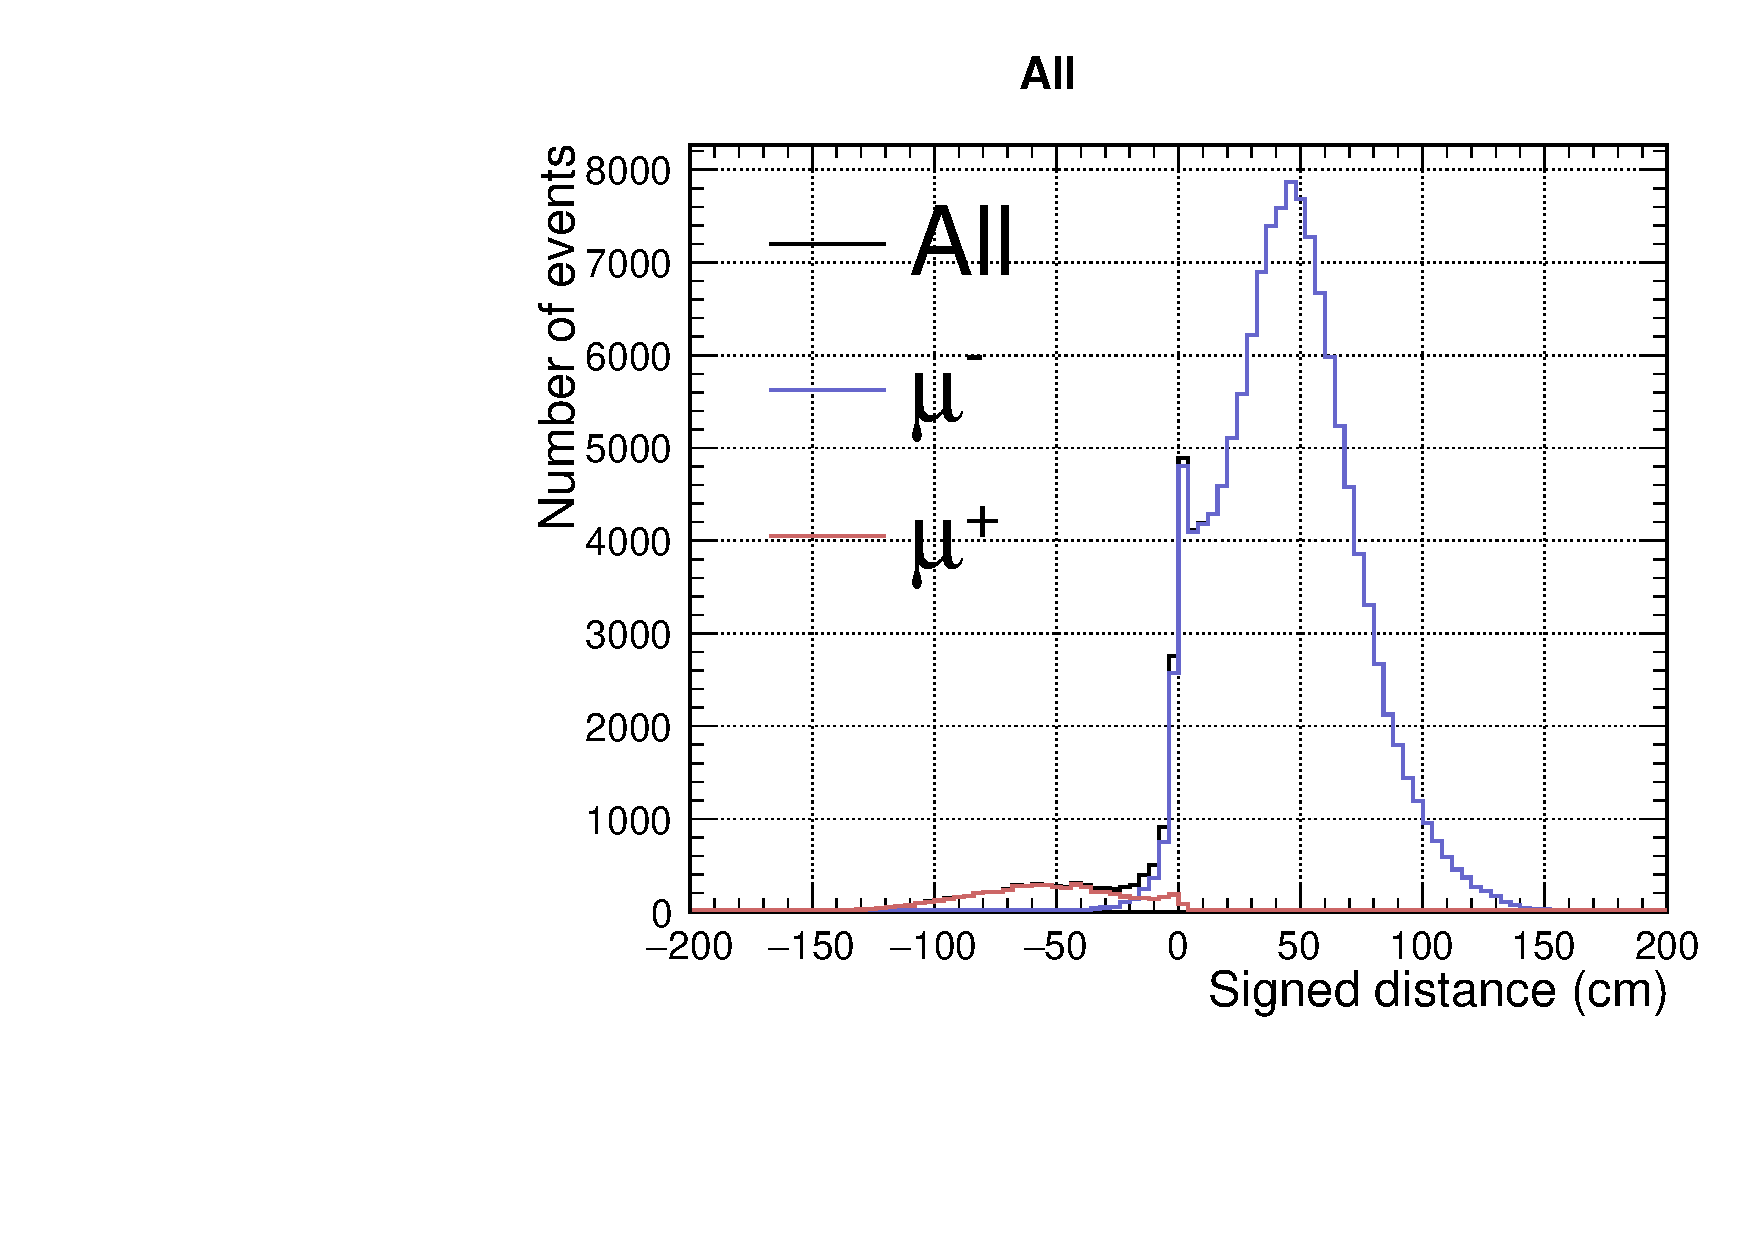
\includegraphics[width=0.65\textwidth, clip, trim={0mm 0mm 0mm 10mm}]{graphics/tms/Simulation/Bend/cmetric_signed_distance.pdf}
\end{dunefigure}

The results from Figure \ref{fig:bend_results} are tabulated in Table \ref{tab:muon_bend}. Firstly, we note the peaks at $\pm50\text{ cm}$, meaning the contained muons on average bend 50 cm in the modules. We observe a mis-identification rate of 3.4\% and 1.9\% for $\mu^-$ and $\mu^+$ respectively in \dword{fhc}. Figures \ref{fig:bend_results_mum} and \ref{fig:bend_results_mup} show that the mis-identification of the lepton charge predominantly happens when the \dword{tms} entrance kinetic energy is below 500 MeV. If a requirement is made on the \dword{tms} entrance kinetic energy at 500 MeV, the $\mu^-$ mis-identification rate falls to 0.8\%, and at 1 GeV it is 0.3\%; for $\mu^+$ the mis-identification rate falls to 0.4\% and 0.2\% with the 0.5 and 1 GeV cuts respectively. As reconstruction improves, we expect this mis-identification rate to improve, but as is the high mis-identification is in a region largely away from the 1st oscillation maximum. 

% These are using Clarence's metric without discretisation
% Tom - compressed the table removing the wrong sign values
% since they are just 1 minus the large value. Can be reverted by removing the % beginning the lines. Also added "inclusive" instead of "---"
\begin{dunetable}
[Fraction of correctly-assigned events with their calculated signed distance for $\mu^{\pm}$]
{cccc}
{tab:muon_bend}
{Fraction of correctly-assigned events with their calculated signed distance for $\mu^{\pm}$ in the \dword{tms}, with requirements on true kinetic energy included. The fractions can be deduced from Figures \ref{fig:bend_results_mum} and \ref{fig:bend_results_mup}.}
Particle & Signed Distance & $T^{TMS}_\mu$ & Fraction \\
\multirow{3}{*}{$\mu^-$} & \multirow{3}{*}{$SD>0$} & Inclusive & 96.6\% \\
%$\mu^-$ & $SD<0$ & --- & 3.4\% \\ \colhline
&& $> 0.5 \text{ GeV}$ & 99.2\% \\ 
%$\mu^-$ & $SD<0$ & $> 0.5 \text{ GeV}$ & 0.8\% \\ \colhline
&& $> 1.0 \text{ GeV}$ & 99.7\% \\
%$\mu^-$ & $SD<0$ & $> 1.0 \text{ GeV}$ & 0.3\% \\ \colhline 
\colhline 
%$\mu^+$ & $SD>0$ & --- & 1.9\% \\ \colhline
\multirow{3}{*}{$\mu^+$} & \multirow{3}{*}{$SD<0$} & Inclusive & 98.1\% \\
%$\mu^+$ & $SD>0$ & $> 0.5 \text{ GeV}$ & 0.4\% \\ \colhline
&& $> 0.5 \text{ GeV}$ & 99.6\% \\ 
%$\mu^+$ & $SD>0$ & $> 1.0 \text{ GeV}$ & 0.2\% \\ \colhline
&& $> 1.0 \text{ GeV}$ & 99.8\% \\ 
% no \colhline on final row
\end{dunetable}

% These are using Clarence's metric, this table includes discretisation in x (but not z)
\iffalse
\begin{dunetable}
[]
{cccc}
{tab:muon_bend}
{Fraction of events with their calculated signed distance for $\mu^{\pm}$ in the \dword{tms}, with cuts on true kinetic energy included. The fractions can be deduced from Figures \ref{fig:bend_results_mum} and \ref{fig:bend_results_mup}.}
Particle & Signed Distance & $T^{TMS}_\mu$ & Fraction \\ \toprowrule
$\mu^-$ & $SD>0$ & --- & 94.7\% \\ \colhline
$\mu^-$ & $SD<0$ & --- & 4.1\% \\ \colhline
$\mu^-$ & $SD=0$ & --- & 1.2\% \\ \colhline

$\mu^-$ & $SD>0$ & $> 0.5 \text{ GeV}$ & 98.6\% \\ \colhline
$\mu^-$ & $SD<0$ & $> 0.5 \text{ GeV}$ & 1.3\% \\ \colhline
$\mu^-$ & $SD=0$ & $> 0.5 \text{ GeV}$ & 0.1\% \\ \colhline

$\mu^-$ & $SD>0$ & $> 1.0 \text{ GeV}$ & 99.2\% \\ \colhline
$\mu^-$ & $SD<0$ & $> 1.0 \text{ GeV}$ & 0.8\% \\ \colhline \colhline 

$\mu^+$ & $SD>0$ & --- & 2.5\% \\ \colhline
$\mu^+$ & $SD<0$ & --- & 96.4\% \\ \colhline
$\mu^+$ & $SD=0$ & --- & 1.1\% \\ \colhline

$\mu^+$ & $SD>0$ & $> 0.5 \text{ GeV}$ & 1.2\% \\ \colhline
$\mu^+$ & $SD<0$ & $> 0.5 \text{ GeV}$ & 98.7\% \\ \colhline
$\mu^+$ & $SD=0$ & $> 0.5 \text{ GeV}$ & 0.1\% \\ \colhline

$\mu^+$ & $SD>0$ & $> 1.0 \text{ GeV}$ & 1.2\% \\ \colhline
$\mu^+$ & $SD<0$ & $> 1.0 \text{ GeV}$ & 98.8\% \\ 
% no \colhline on final row
\end{dunetable}
\fi

\begin{dunefigure}[Entrance muon kinetic energy for $\mu^-$ with positive and negative signed distance]{fig:bend_results_mum}
{The distribution of true \dword{tms} entrance muon kinetic energy for $\mu^-$ with positive and negative signed distance is shown on the left with the fraction of each shown on the right. The wrongly assigned signed distance ($SD<0$ for $\mu^-$) happens predominantly at low muon kinetic energy, and is mostly gone by 1 GeV.}
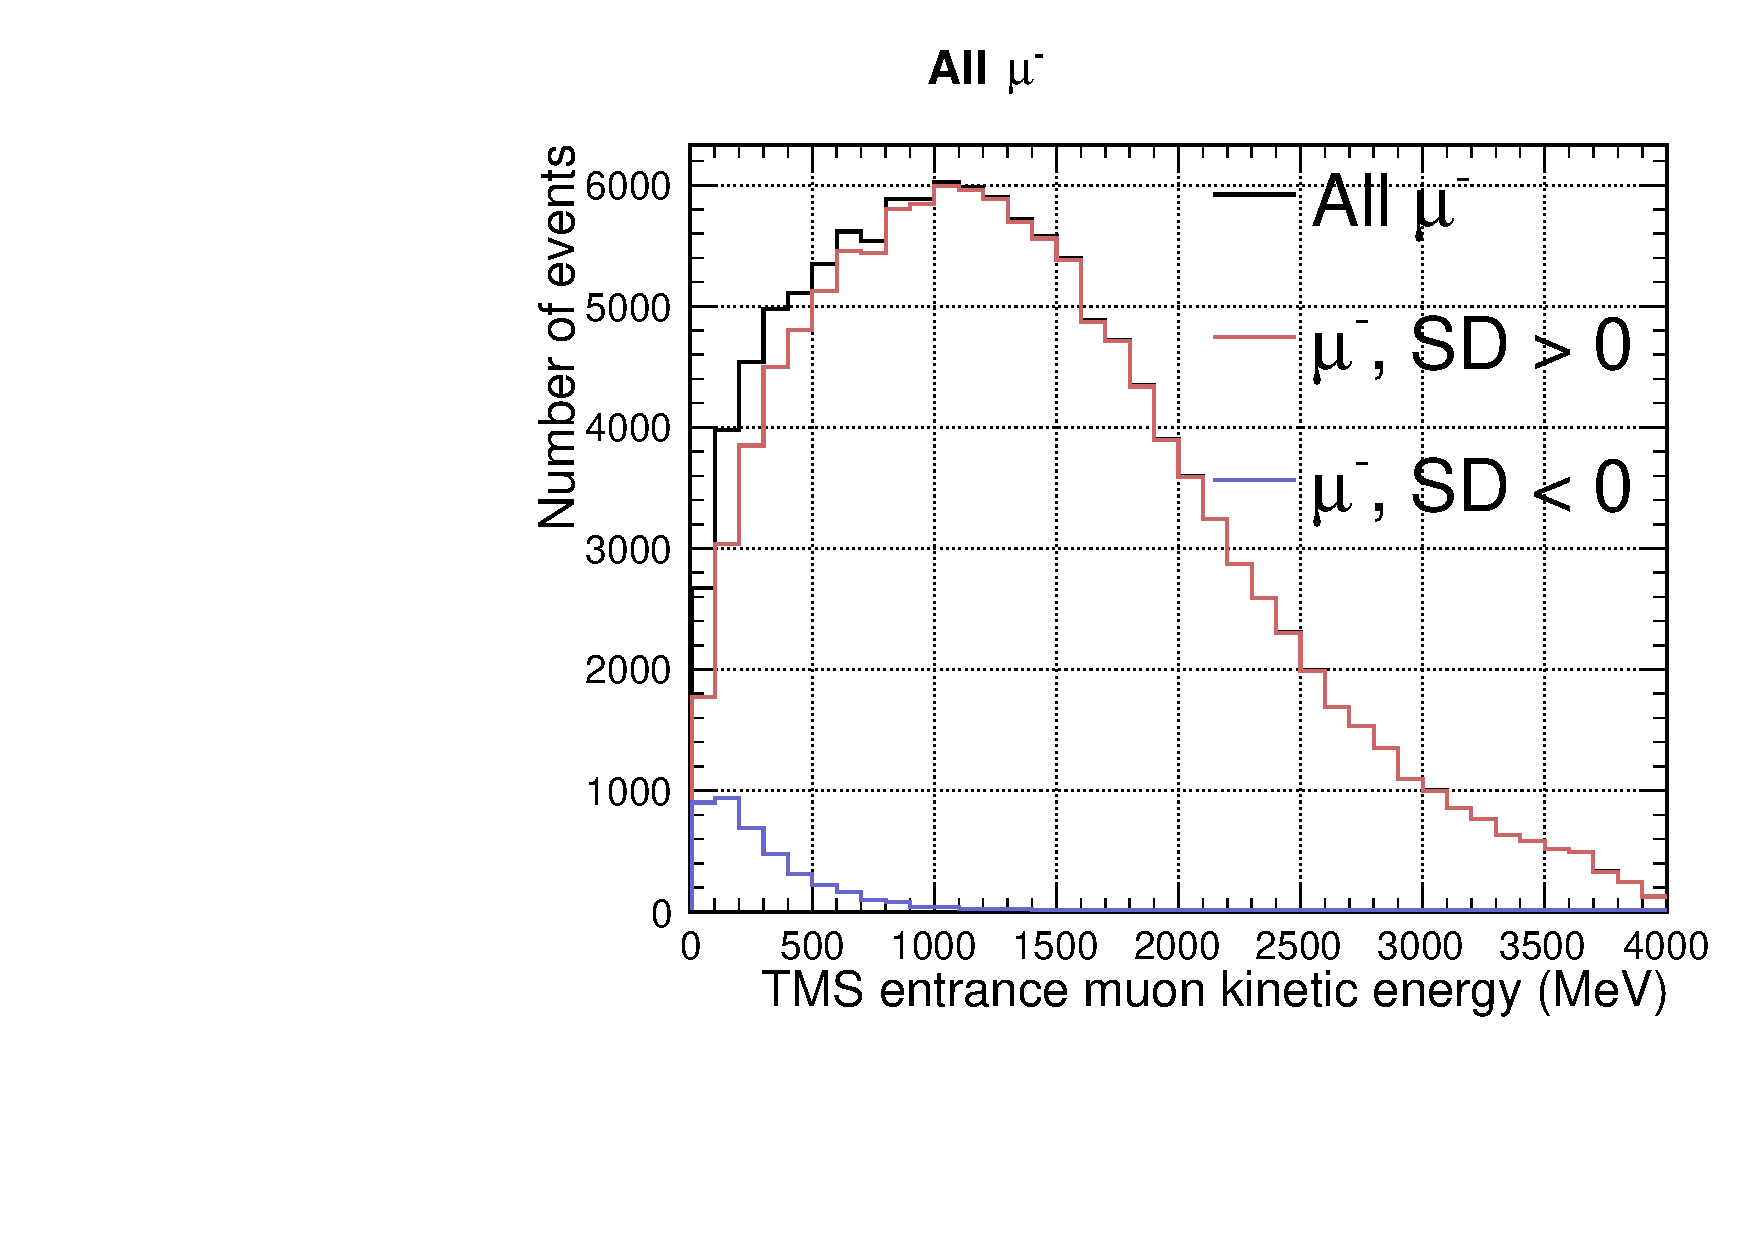
\includegraphics[width=0.49\textwidth, clip, trim={0mm 0mm 0mm 10mm}]{graphics/tms/Simulation/Bend/cmetric_signed_distance_KE.pdf} 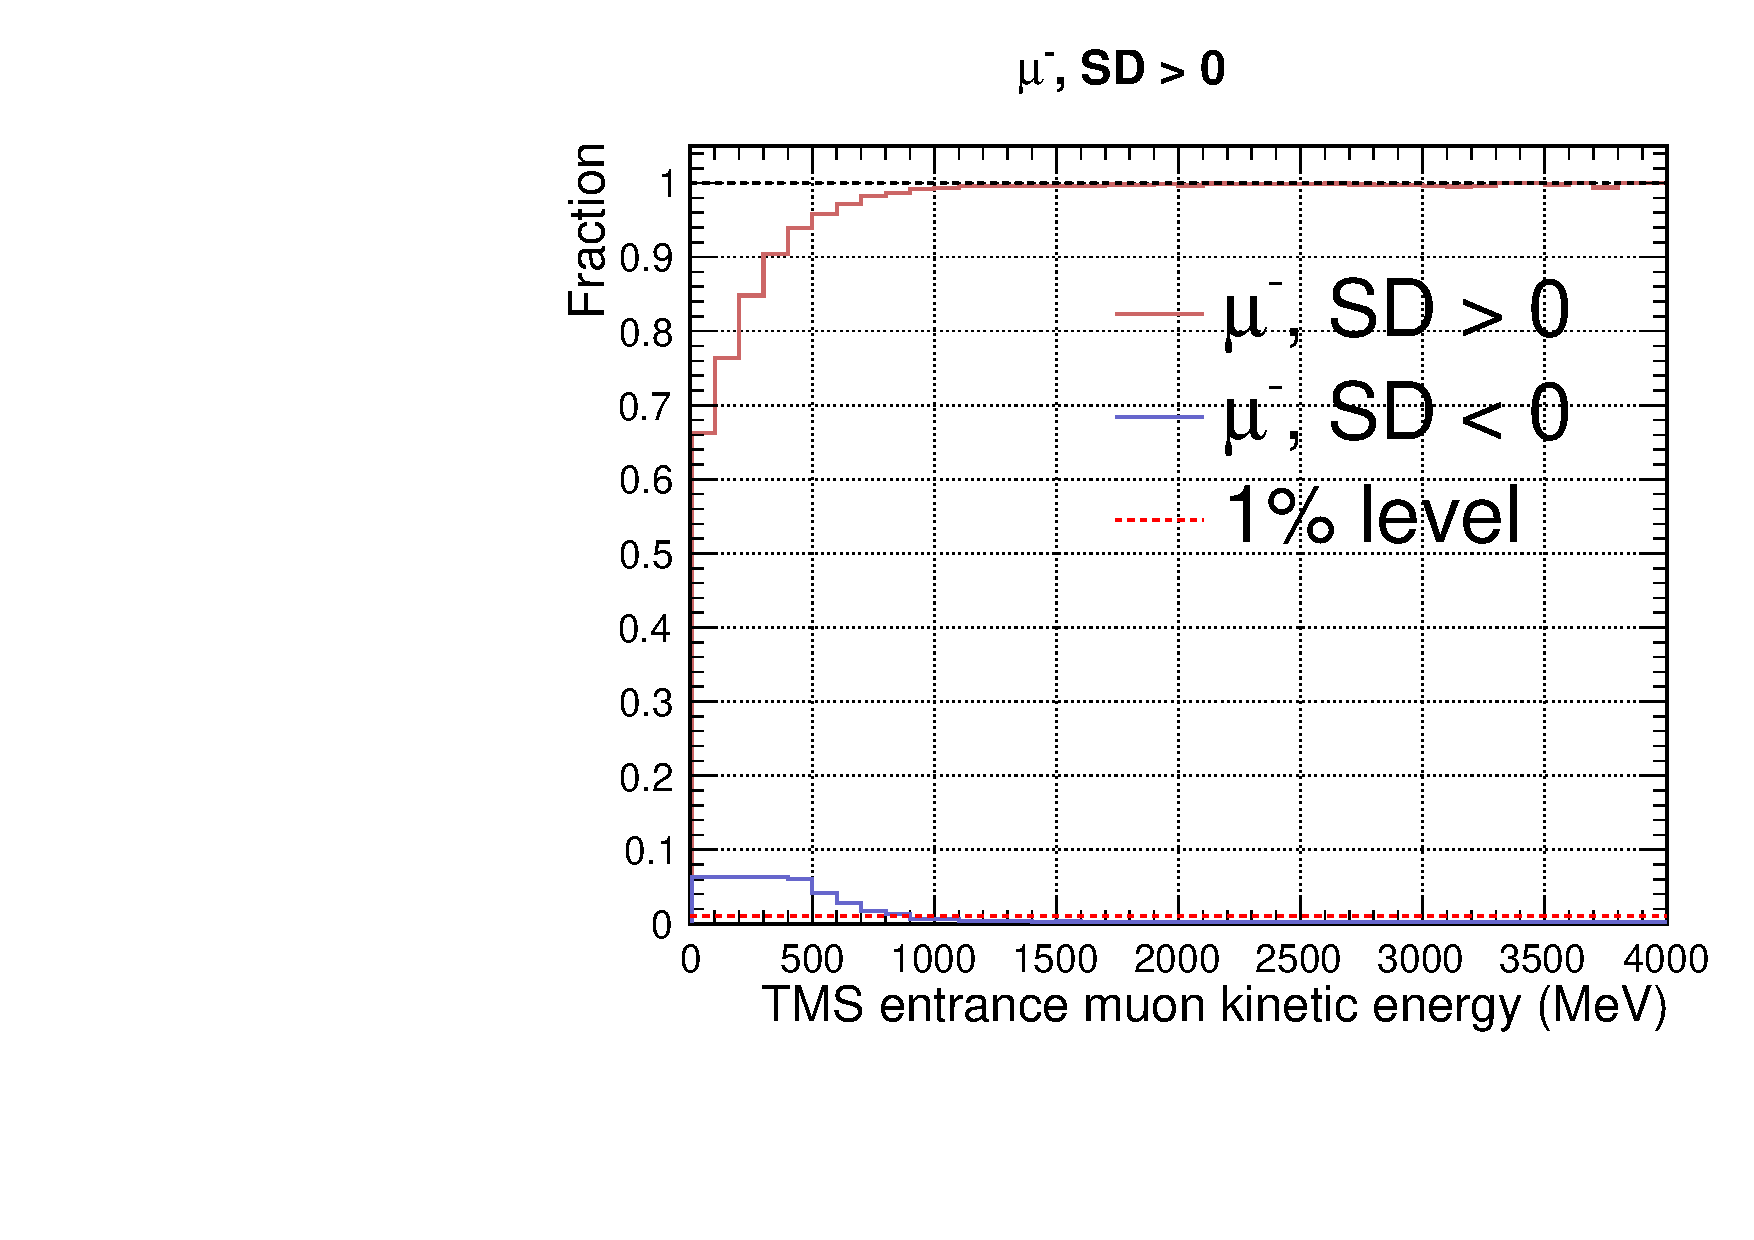
\includegraphics[width=0.49\textwidth, clip, trim={0mm 0mm 0mm 10mm}]{graphics/tms/Simulation/Bend/cmetric_signed_distance_KE_ratio.pdf}
\end{dunefigure}

\begin{dunefigure}[Entrance muon kinetic energy for $\mu^+$ with positive and negative signed distance]{fig:bend_results_mup}
{The distribution of true \dword{tms} entrance muon kinetic energy for $\mu^+$ in \dword{fhc} with positive and negative signed distance is shown on the left with the fraction of each shown on the right. The wrongly assigned signed distance ($SD>0$ for $\mu^+$) happens predominantly at low muon kinetic energy, and is mostly gone by 500 MeV.}
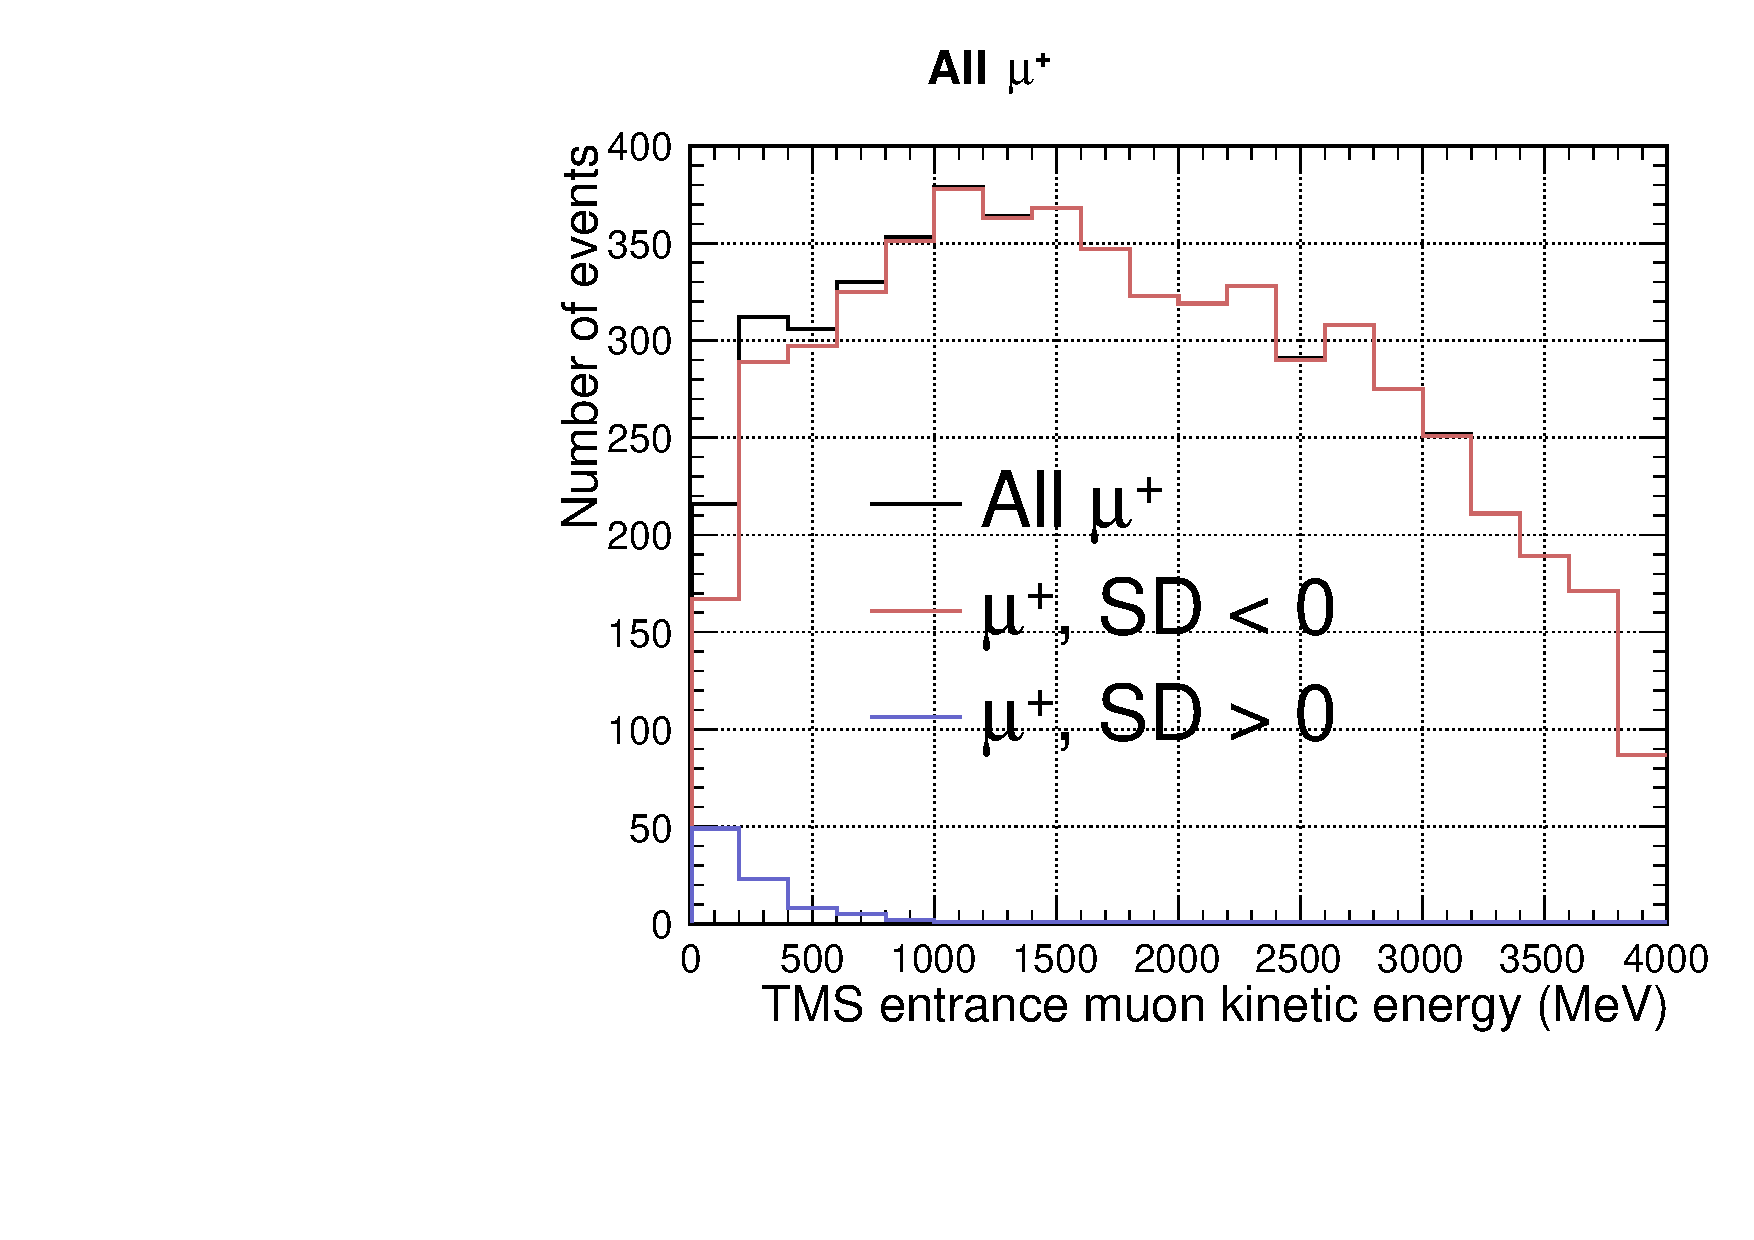
\includegraphics[width=0.49\textwidth, clip, trim={0mm 0mm 0mm 10mm}]{graphics/tms/Simulation/Bend/cmetric_signed_distance_KE_muplus.pdf} 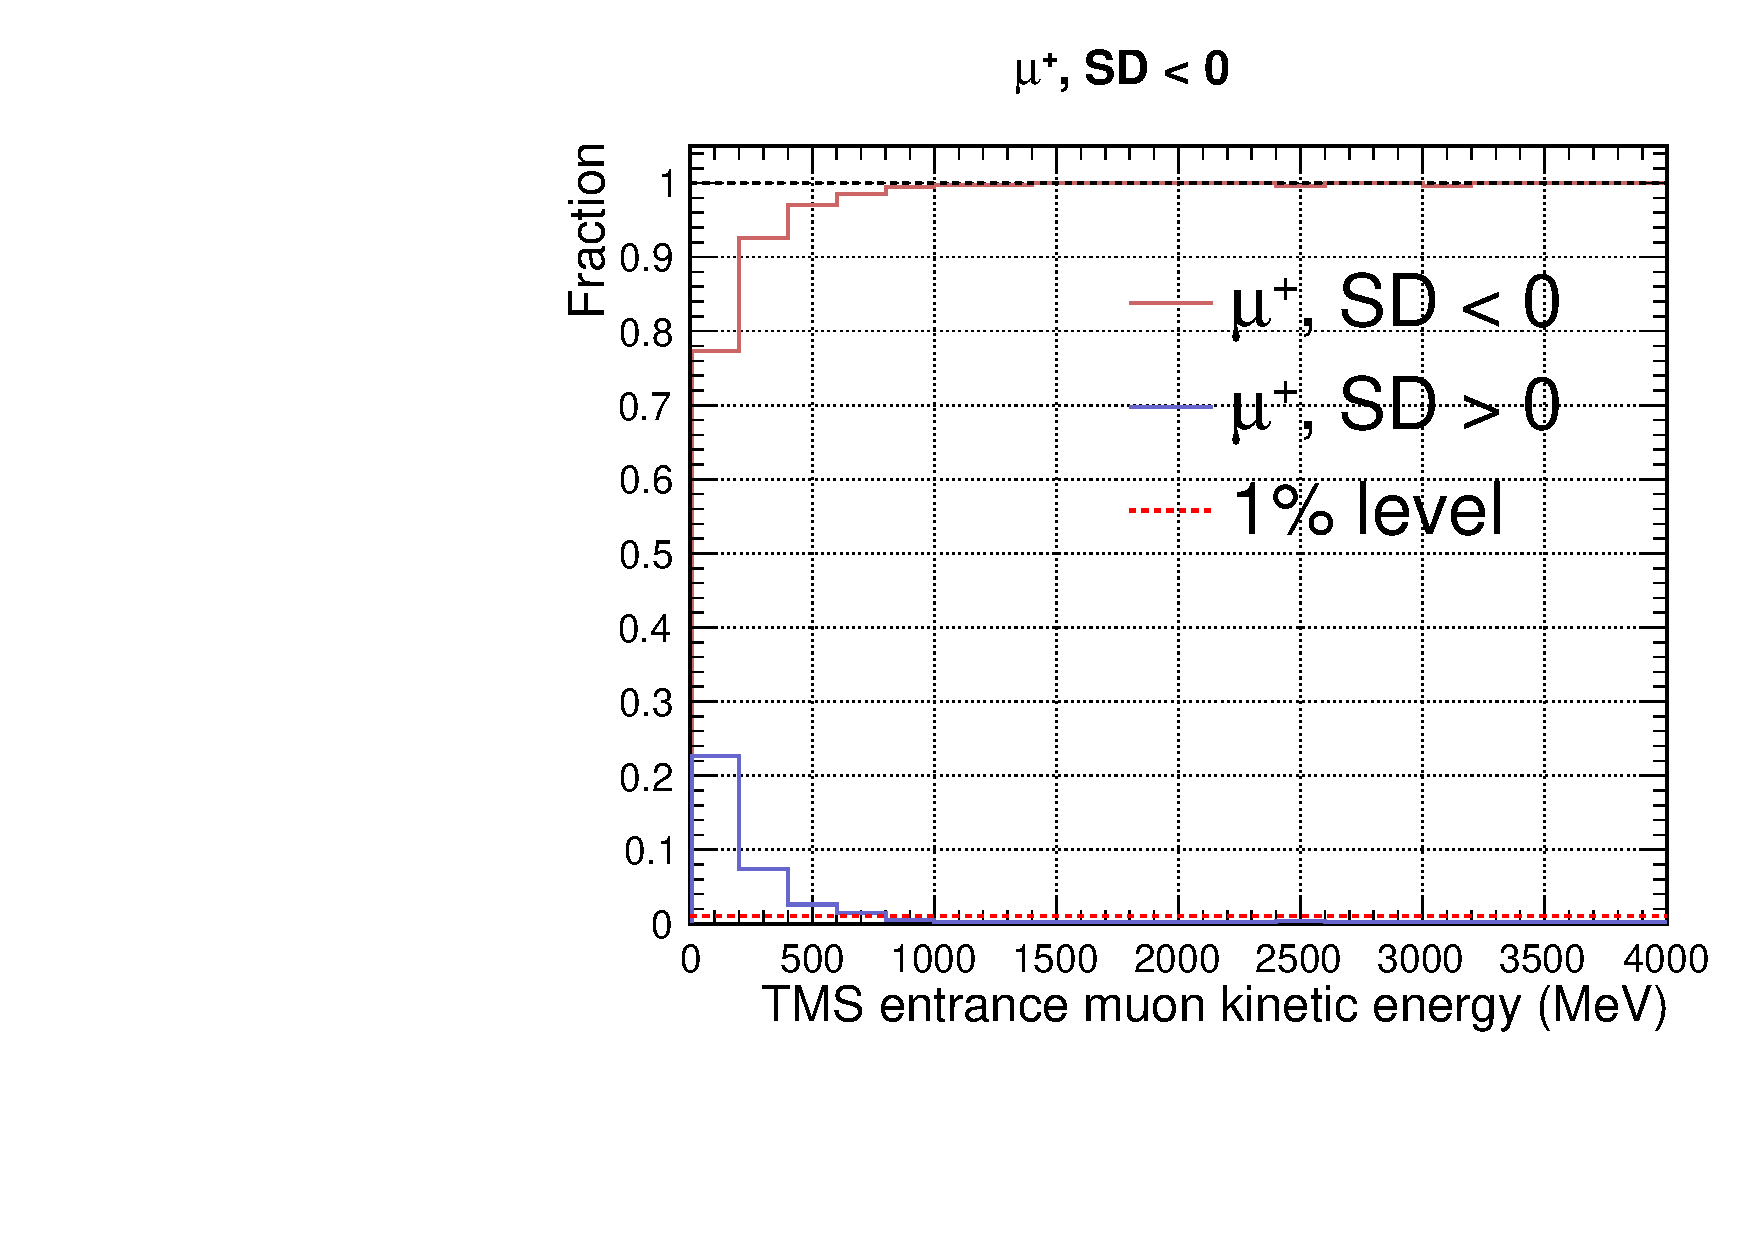
\includegraphics[width=0.49\textwidth, clip, trim={0mm 0mm 0mm 10mm}]{graphics/tms/Simulation/Bend/cmetric_signed_distance_KE_muplus_ratio.pdf}
\end{dunefigure}

% These are using Gavin's signed distance metric
\iffalse
\begin{dunetable}
[Fraction of events with signed distance for $\mu^{\pm}$.]
{cccc}
{tab:muon_bend}
{Fraction of events with their calculated signed distance for $\mu^{\pm}$ in the \dword{tms}, including the effects of cuts on the true kinetic energy in the \dword{tms}.}
Particle & Signed Distance & $T^{TMS}_\mu$ & Fraction \\ \toprowrule
$\mu^-$ & $SD>0$ & & 95.4\% \\ \colhline
$\mu^-$ & $SD<0$ & & 4.6\% \\ \colhline
$\mu^-$ & $SD>0$ & $> 0.5 \text{ GeV}$ & 98.0\% \\ \colhline
$\mu^-$ & $SD<0$ & $> 0.5 \text{ GeV}$ & 2.0\% \\ \colhline
$\mu^-$ & $SD>0$ & $= 1.0 \text{ GeV}$ & 99.1\% \\ \colhline
$\mu^-$ & $SD<0$ & $= 1.0 \text{ GeV}$ & 0.9\% \\ \colhline
$\mu^+$ & $SD>0$ & & 4.0\% \\ \colhline
$\mu^+$ & $SD<0$ & & 96.0\% \\ % no \colhline on final row
\end{dunetable}
\fi


%\label{sec:tms-ovvw-perf}
%%%%%%%%%%%%%%%%%%%%%%%%%%%%%%%%
\subsubsection{Progress toward Reconstruction}

The output of the \dword{tms} reconstruction will inform the \dword{ndlar} reconstruction as to which tracks exited the \dword{ndlar} and were reconstructed in the \dword{tms}. However, the \dword{tms} will also be able to run a stand-alone reconstruction. Our end vision of the \dword{ndlar} and \dword{tms} system is to first run both detectors' reconstruction separately, then informing the \dword{ndlar} of the most likely muon track in the \dword{tms}, followed by the \dword{ndlar} reconstruction propagating its estimates of the same muon candidate back into the \dword{tms} reconstruction for an improved \dword{tms} estimate. This process can be iterative and run in forward and back-propagating modes. A stand-alone \dword{tms}-reconstruction also enables monitoring of the inclusive neutrino event rate, using neutrinos interacting on the \dword{tms} fiducial volume.

The \dword{tms} reconstruction is in progress. The current approach is investigating running the track finding and reconstruction simultaneously through a Kalman filter, or having a separate track finding algorithm identify track candidates which it feeds to the Kalman track reconstruction.

\subsubsubsection{Track finding}
For the track finding stage, we are currently investigating three approaches. They all run in each view separately, and the 2D to 3D track matching and merging is done at a later stage.

\begin{itemize}
    \item Perform a Hough transform \cite{hough} in each view separately, and find which hits intersect the primary Hough line. Traverse the hits and group neighbouring hits into a track candidate. Take remaining hits (not belonging to a candidate) and repeat process to see if there is a $N^{th}$ track candidate. Due to the bending in the $x-z$ view, the Hough transform is often more successful in the $y-z$ view, and the neighbour clustering in $x-z$ is critically important.

    \item Sort the hits in $z$, and run a custom A* path finding algorithm from first to last hit in $z$. The intent is to find the shortest path between the first and last hit, only traversing cells that have been hit. If no path is found from start to finish, repeat A* path finding running until the hit with second largest z, and continue.
    
    \item Sort the hits in $z$, and run a Kalman filter from first to last hit in $z$. For this to succeed, the Kalman filter needs to account for the energy-loss, bending and multiple-scattering happening in the iron and scintillator layers. 
\end{itemize}

The track finding will benefit from $y-z$ and $x-z$ views communicating to correctly identify particles based on their range in z, for instance making sure the longest track candidate has similar start and end positions in both views. This is particularly useful to find the endpoint of a track in $x-z$ using the $y-z$ view, since the end of a track in $x-z$ is often bent significantly due to the magnetic field. 

We envisage using bifurcations in track candidates to tag non-muons (as muons rarely undergo secondary interactions, compared to pions), and split candidates into separate track candidates if the bifurcation is $N$ planes long.

One of the track finding algorithms (Hough transform followed by adjacent merging) is shown in Figure \ref{fig:track_Hough_1} for a single and a two track event. The single track event is particularly difficult single-track events as they traverse the gap region so have discontinuities in both views. The Hough transform correctly identifies the dominant straight line hits of the track, and the subsequent neighbour clustering finds the hits across the gap regions. A clear strength of the Hough transform is its ability to clearly recognise separate straight tracks.
\begin{dunefigure}[Hough track finding algorithm for single and a two track event.]{fig:track_Hough_1}
{One single-track and one two-track event in the \dword{tms}, where tracks are found by the Hough+clustering algorithm, showing $x-z$ (left) and $y-z$ (right) hits. The green and red boxes show the total and fiducial volume respectively, the vertical dashed gray line shows the region where the \dword{tms} transitions from thin to thick iron layers, and the three horizontal white dotted regions in the $x-z$ view shows the gap region. The yellow fills show the hits that were found by the procedure. The $x-z$ view shows the tracks traversing the central and lower gap region respectively, leaving a broken track in both views. Despite this, the Hough transform and adjacent hit merging finds all relevant hits in the track. N.B. the detector coordinate system differs from the event displays by being in mm (not cm) and translated by $\{x,y,z\}=\{0, 5, 411\}$ mm. }
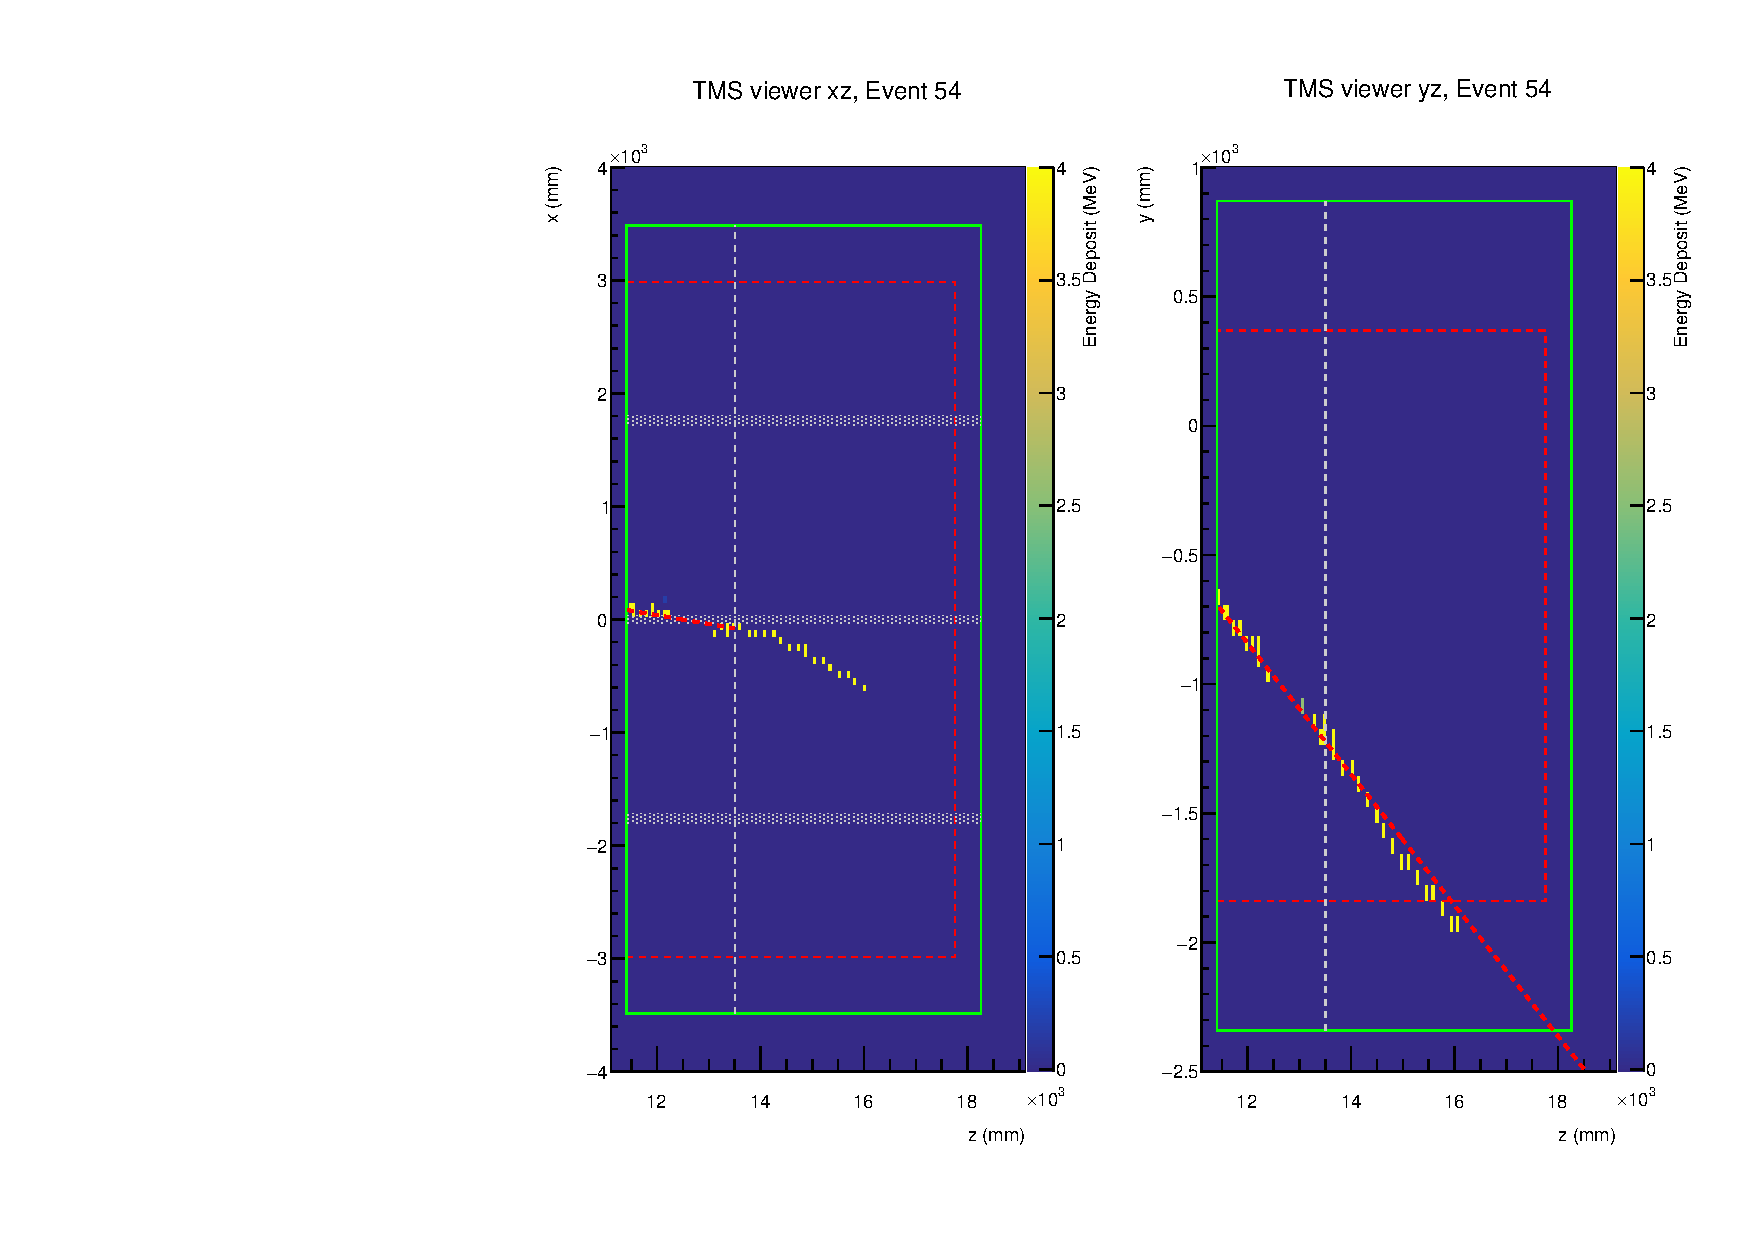
\includegraphics[width=0.49\textwidth]{graphics/tms/Simulation/Hough/Hough_Example.pdf} 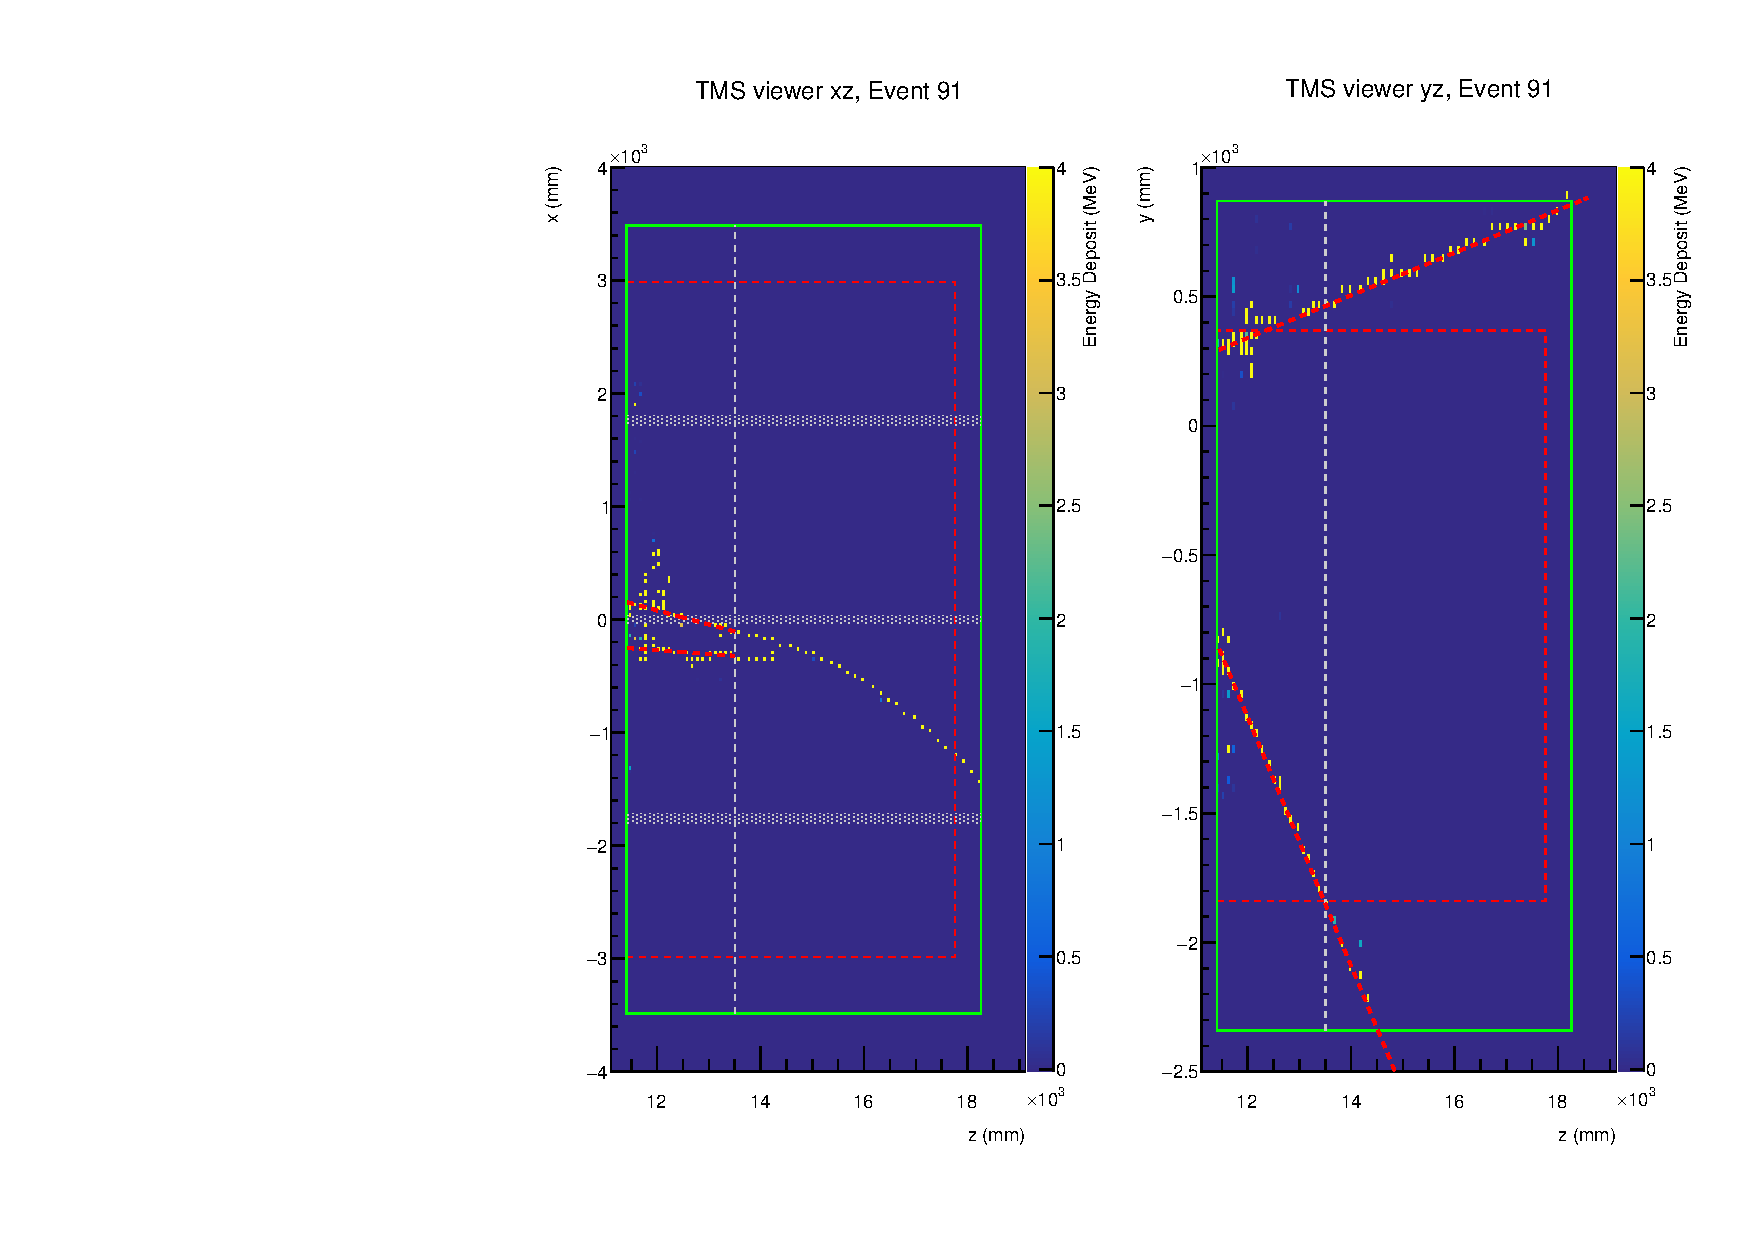
\includegraphics[width=0.49\textwidth]{graphics/tms/Simulation/Hough/2track_hough_2.pdf}
\end{dunefigure}

An example of the A* track finding is shown in Figure \ref{fig:track_astar_1}, finding the optimal path between the last and first hit in $z$ separately in both views. It does so by choosing the path that minimises the cost related to connecting nearby cells, accounting for the change in distance from the goal cell. 
%The implementation in \texttt{TMS\_Reco} allows switching A* to a greedy best-first search, where the distance to the goal cell is the only metric, and there is no cost incurred from connecting cells.
\begin{dunefigure}[A* track finding algorithm for single track events.]{fig:track_astar_1}
{Two single-track events in the \dword{tms}, where tracks are found by A* path-finding algorithm, showing $x-z$ (left) and $y-z$ (right) hits. The green and red boxes show the total and fiducial volume respectively, the vertical dashed gray line shows the region where the \dword{tms} transitions from thin to thick iron layers, and the three horizontal white dotted regions in the $x-z$ view shows the gap region. The yellow fills show the hits that were found by the procedure. The right-most event has a clear secondary interaction, where the path bends abruptly in the $y-z$ view. N.B. the detector coordinate system differs from the event displays by being in mm (not cm) and translated by $\{x,y,z\}=\{0, 5, 411\}$ mm. }
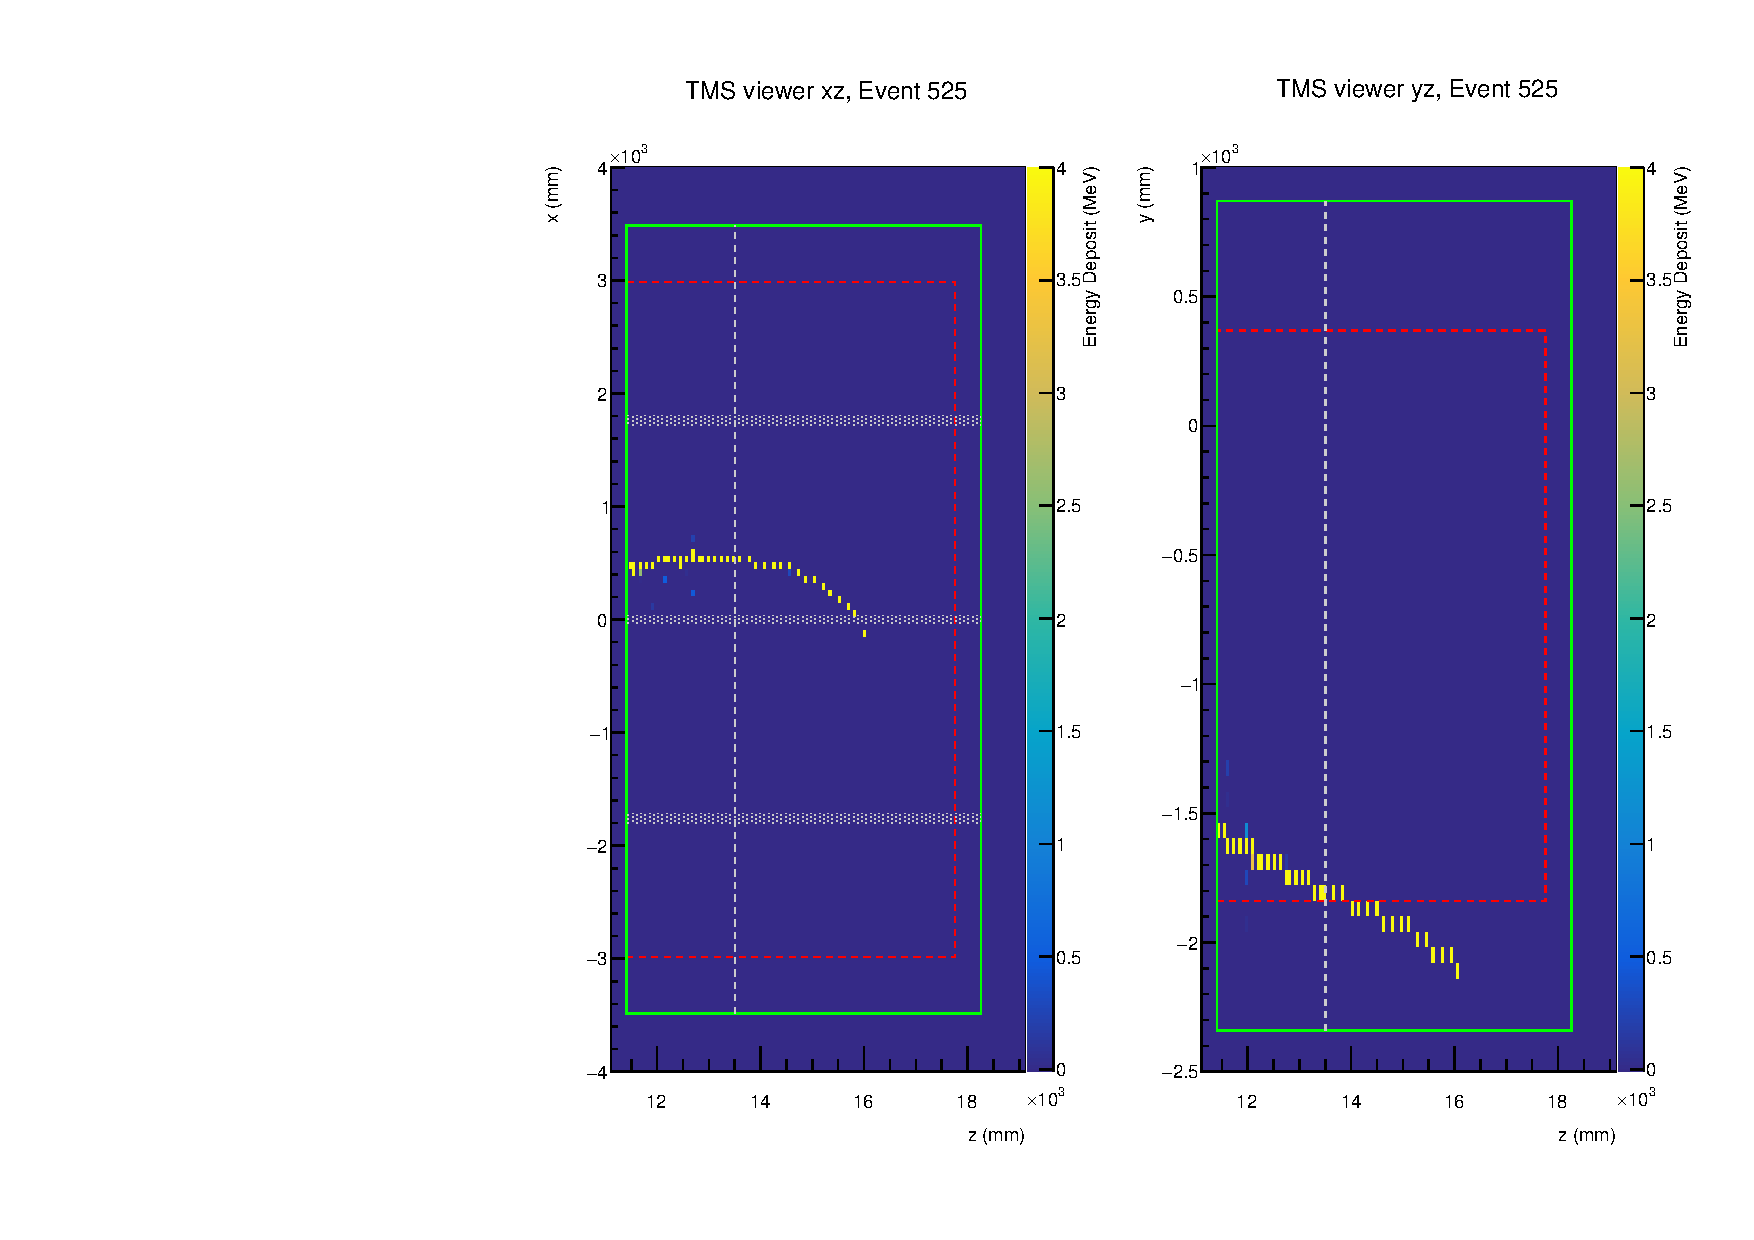
\includegraphics[width=0.49\textwidth]{graphics/tms/Simulation/Astar/track_example_astar2.pdf} 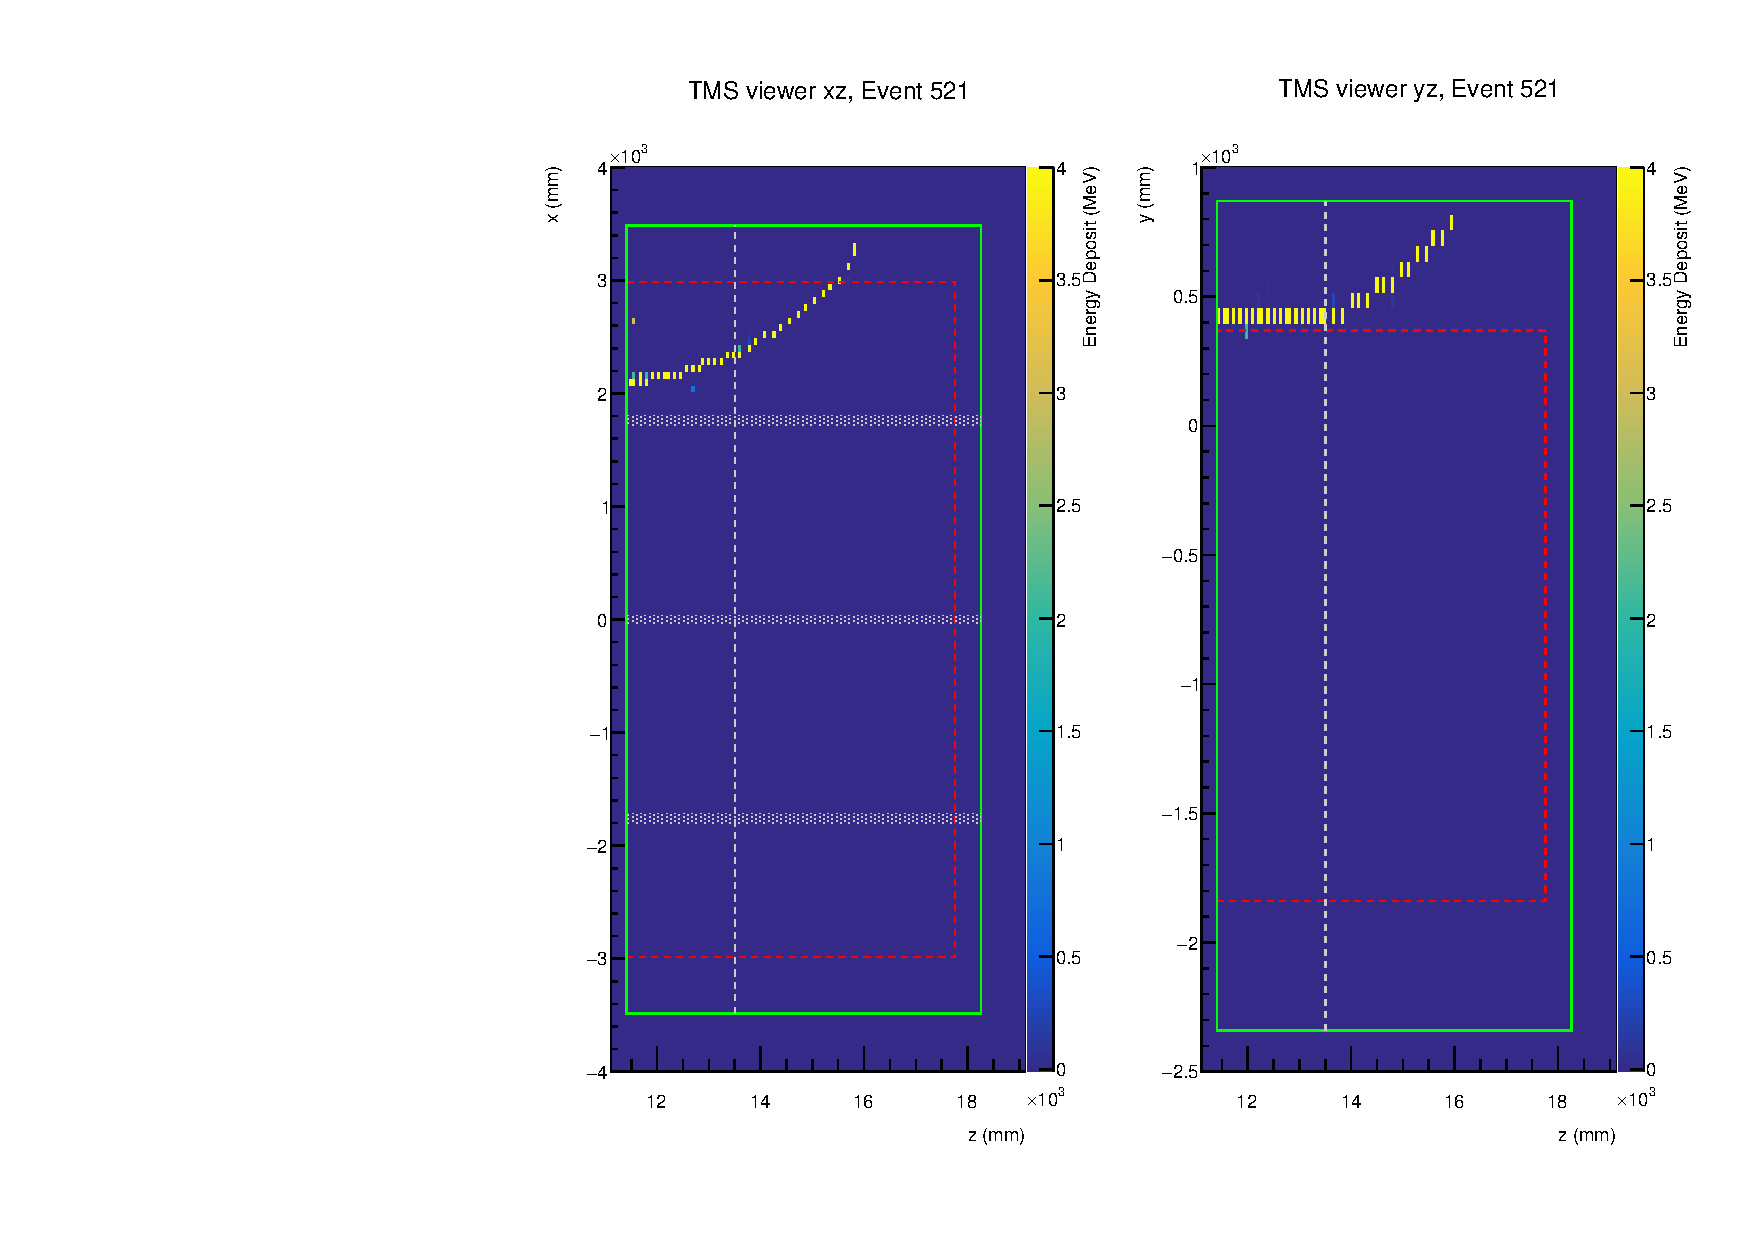
\includegraphics[width=0.49\textwidth]{graphics/tms/Simulation/Astar/track_example_astar3.pdf}
\end{dunefigure}

\subsubsubsection{Track reconstruction}
Currently, the lepton candidate is assumed to be the longest track in the track finding. After the reconstruction stage, it is envisioned the lepton candidate is assumed to be the most energetic track that fits a muon hypothesis. Depending on the final design of the \dword{tms}, the track reconstruction will operate on 2D or be combined into 3D views. 

Preliminary studies show track length is by far the most important feature for a good muon KE measurement, with the energy deposits and track bending being secondary contributions. The current Kalman implementation in the \dword{tms} software includes effects from energy loss and multiple scattering, inspired by similar implementations in \dword{minos}, \dword{minerva}, and \dword{t2k}. Efforts towards integration of the \dword{ndlar} and \dword{tms} reconstructions are also ongoing.

%\subsubsubsection{Integration with \dword{ndlar}}
%\fixme{Chris to write about LAr integration}

%%%%%%%%%%%%%%%%%%%%%%%%%%%%%%%%
\section{System Design}
\label{sec:tms-des}

%%%%%%%%%%%%%%%
\subsection{Transition Path to ND-GAr}
\label{sec:tms-des-path}

A unique aspect of the \dword{tms}
is that it is temporary. It will operate for a few
years and then be replaced by the more capable 
\dword{ndgar}. This relaxes certain requirements,
for example the need to operate at a beam power of 2.4\,MW (something planned to happen beginning in year six) but imposes others, such as the need
to be removed with minimal impact to experiment
operations.

The replacement of the \dword{tms} by \dword{ndgar} can be
accomplished in about two weeks. The procedure is
to build \dword{ndgar} on the west \dword{duneprism} rails. When
complete, temporary rail crossings between
the \dword{duneprism} east and west rails are installed,
the \dword{tms} is then disconnected and using these
rails moved from the west to east rails. From
there, \dword{tms} moves north on the west rails and
\dword{ndgar} south on the east rails. Then
\dword{ndgar} begins operation and \dword{tms} begins
disassembly.

During the \dword{ndgar} construction and \dword{tms} disassembly, the
\dword{duneprism} range of motion is reduced by about eight meters. It
would be possible to take additional running at the extreme
north position immediately before and after this period of restriction.

%%%%%%%%%%%%%%% One for each WBS element
%%%%%%%%%% The P6 WBS is not useful for this, as it breaks the work down
%%%%%%%%%%  by time, not activity
\subsection{Support Structure}
\label{sec:tms-des-structure}
The mechanical design consists of 2 parts, a steel support frame and a series of layered steel plates.  The support frame has four legs tied together with steel diagonal bracing. Bolted to the top of the legs are two beams W27 $\times$ 114, spaced \SI{6400}{\mm} apart. Transverse to those beams is a bed of five W30 $\times$ 191 beams evenly spaced. At the end of the transverse beams, bolted to the top, is a strong back consisting of two W8 $\times$ 24 beams tilted back at \SI{1.5}{\degree}. The bottom of the legs have heavy duty Hilman rollers to allow the frame to be moved using hydraulic cylinders.

%%%%%%%%%%%%%%%
%To keep the plates from sliding, bolted to the W30 beams between each layer is a block \SI{38}{\mm} $\times$ \SI{25}{\mm} $\times$ \SI{177}{\mm}. 
%To maintain the \SI{40}{\mm} spacing and to anchor the plates, they are bolted together with spacer blocks in four equally spaced locations at the perimeter of the plates. The spacer blocks are drilled at a \num{1.5} degree angle and each bolt screws into the head of the previous bolt. 

%\begin{dunefigure}[Optional short caption for LoF]{fig:required-label}
%{Required full caption.}
%
\includegraphics[width=0.8\textwidth]{dunelogo_colorhoriz}
%\end{dunefigure}

An analysis was carried out to ensure that this support structure satisfies the AISC design provisions for the given loading conditions.  The analysis was performed with a combination of hand calculations and finite element modeling with SAP2000 %\cite{SAP2000}.  
Structural steel construction specifications from the American Institute of Steel Construction (AISC 360-16 
%\cite{AISC360-16}
) were used as the guide for the strength design.  The design check takes into account all local member details, including lateral torsional buckling, local buckling effects depending on the member shapes, etc. as required by the AISC code, and determines which sections pass or fail the design check. Every structural member passes the design check based on the AISC design standards for combined axial loading and bi-axial bending.  The support structure was also checked for stability over tipover forces along the guided direction and the perpendicular direction for a nominal seismic force.   The smallest force required to tip the structure over was calculated about the right support, at 623 kips. The seismic force was calculated with 20\% of the weight of the structure, 238.2 kips, applied as a pseudo-static horizontal force applied at the center of gravity.
   
% some of Figures 6-8

%%%%%%%%%%%%%%%  One for each WBS element
\subsection{Detector Steel}
\label{sec:tms-des-steel}

The second part of the mechanical design is a series of \num{100} layered plates mounted to the bed of the steel support frame. The downstream \num{60} layers of plates are mounted on edge and lean against the strong back at \num{1.5} degrees. The plates are \SI{40}{\mm} steel and spaced \SI{40}{\mm} apart. The upstream \num{40} layers are \SI{15}{\mm} steel and spaced \SI{40}{\mm} apart. Each layer consists of three plates, two at \SI{1.85}{\m} nominal width and one at \SI{3.7}{\m} nominal width. All the plates are \SI{5.0}{\m} tall. There is a \SI{40}{\mm} horizontal gap between each of the plates.   At the sides of each plate are two notches, \SI{30}{\mm} deep $\times$ \SI{300}{\mm} high, to receive the coils. The coils wrap around each of the three groups of plates.   Figure \ref{fig:tms_anl_fig1} shows the support structure, steel plates, and coils.  


% The coils cost us a bit less than 1% in acceptance.  T
The plates are made from the same 1006 steel used for  MINOS/BaBar which is high silicon, low-carbon, chosen for its magnetic properties ($\mu \ge 700$). 


%%%%%%%%%%%%%%%  One for each WBS element
\subsection{Magnet Coils and Power Supplies}
\label{sec:tms-des-coil}

The magnet has three design goals:
\begin{itemize}
    \item As high a field as possible inside the magnet,
    \item As uniform a field as possible inside the magnet,
    \item As low a field as possible outside the magnet.
\end{itemize}

To reach these goals, each row of steel has two coil wraps to provide a uniform magnetic field, as shown in Figure \ref{fig:tms_anl_fig1}.  
%Figure \ref{fig:tms_anl_coils} is a schematic of the coil and current flow.  
There are two “belts” of coils in a Helmholtz-like configuration which gives a reasonably uniform field, especially between the coils.   This coil and field configuration strikes the balance between a large field inside the spectrometer, while keeping the field inside the \dword{ndlar} as low as possible. The coils will be air-cooled.  

\begin{dunefigure}[Schematic of coil arrangement and current flow]{fig:tms_anl_coils}
{Schematic of coil arrangement and current flow.}
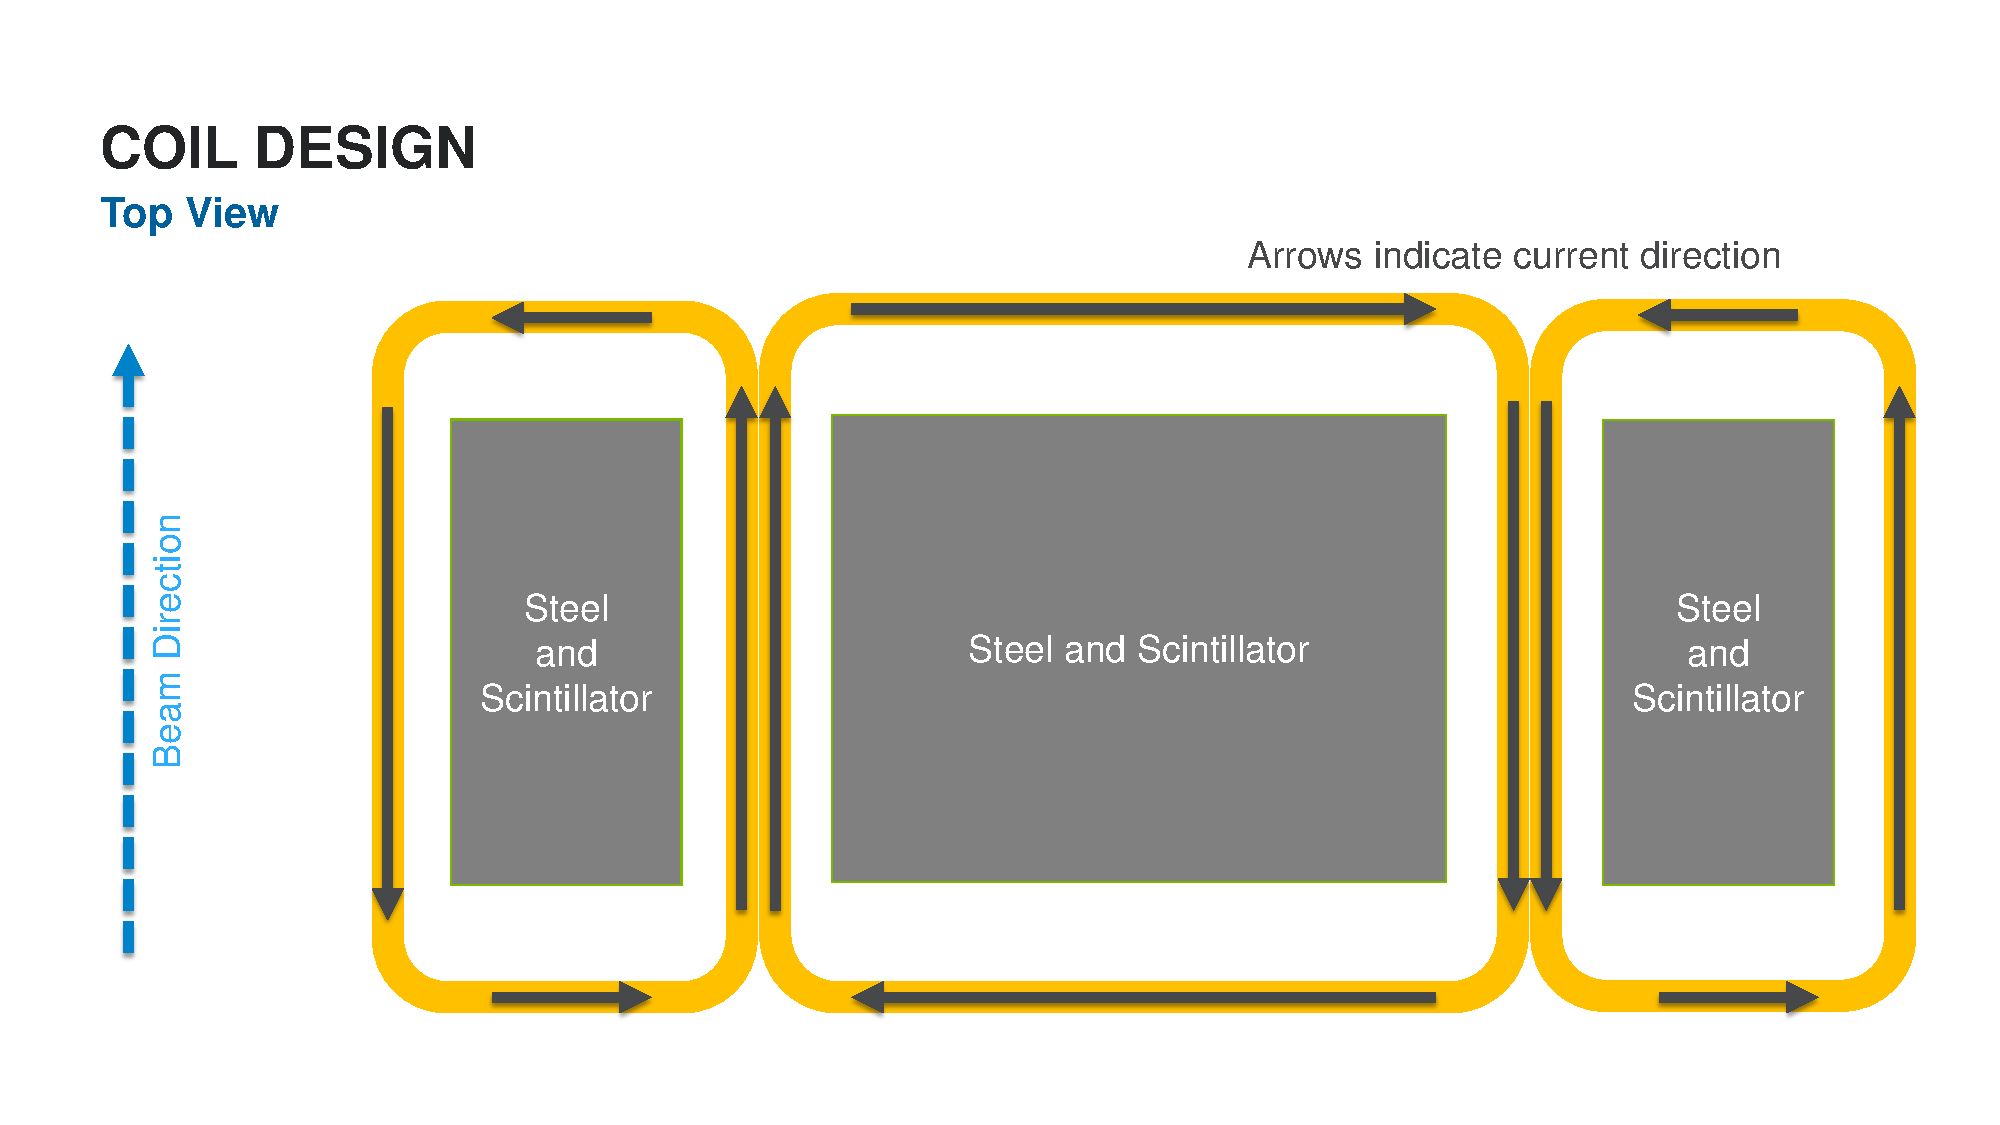
\includegraphics[width=0.9\textwidth]{graphics/tms/Detector/tms_anl_coils.pdf}
\end{dunefigure}

Additionally, there are cost considerations and 
tensions among the ensemble of goals. This design emphasizes
field magnitude, low fringe and low cost over field uniformity. The outer two-quarters of the magnet have a field, nominally vertical, in the opposite direction to the center half. Externally, these fields largely cancel: the dipole component cancels; the quadrupole component largely cancels; and the residual component is a sextupole.

A magnetic analysis was performed with the Low Frequency EMAG module in Ansys Multiphysics \cite{ANSYS}.   The goals of this analysis were to determine the magnetic field intensity and magnetic flux density in the spectrometer, determine the mechanical load due to the magnetic field on the plates, and determine the magnetic field adjacent to the spectrometer.   Each coil in the model consisted of two layers of \num{50} turns of \num{15} $\times$ \SI{10}{\mm} copper bar, giving a cross section of \num{30} $\times$ \SI{500}{\mm}.  The current in each turn was \num{300} A, for a total current of \num{30,000} A. (Various current configurations were modeled, including the present baseline of two hundred turns of 00 gauge insulated wire carrying 150 amperes) The current in each plate bundle flowed in a direction opposite that of the bundle next to it.  The model is a half symmetry, and was split on the global Y-Z plane. Solid geometry of the plates and air were created and then meshed with over four million SOLID96 eight node brick elements.   This model is shown in Figure \ref{fig:tms_anl_Bmodel1}.  Results of the magnetic field simulation are shown in Figure \ref{fig:tms_anl_Bfield1}.   In addition, the magnetic nodal forces were computed and found to be less than 25\% of the maximum pressure value.  
%Clarence put this in to make document compile
\iffalse
%This is shown Error! Reference source not found..  Boundary conditions (Figure 20) were flux-parallel on the symmetry plane and flux normal (MAG = 0) on the far field boundaries.  The flux normal boundary was achieved with INFINIT117 elements.

%The magnetic scalar potential formulation was used. 

%This method supports the use of a coil primitive, and bonded contact between regions in the model.  Due to the unusual range of dimensions in the geometry, these features were crucial to the development of a practical model.  The spectrometer consists of \num{100} thin (\num{20} and \SI{40}{\mm}thick) steel plates with a surface area of nearly \num{11} $m^2$ separated by \SI{40}{\mm} air gaps.  The coil bears directly on the steel plate, with only the insulation, estimated at \SI{1}{\mm} thick, between the copper conductor and the plate.  This four orders of magnitude between dimensions would be difficult to mesh as a single component, and the sheer size of the spectrometer would result in a very large element count.  
%Bonded contact with a magnetic degree of freedom and a coil primitive significantly streamlined the process.

%A model was built in Ansys MAPDL with a script.    The coil was modeled with SOURC36 current source primitive.  Symmetry cannot be applied to SOURC36 elements, so the whole coil is modeled. This model is shown in Figure 18 and the finite element mesh is shown in Figure 19.  
\fi

\begin{dunefigure}[ANSYS model used for the magnetic field simulation.]{fig:tms_anl_Bmodel1}
{ANSYS model used for the magnetic field simulation.  Left:  Solid geometry for the magnetic simulation.  Right:  Finite Element Mesh used in the magnetic field simulation.   }
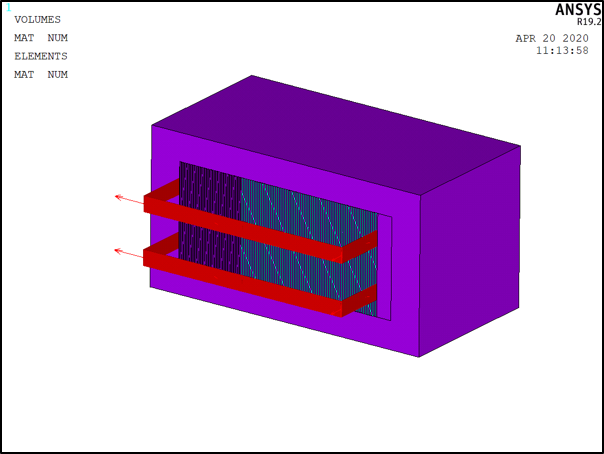
\includegraphics[width=0.49\textwidth]{graphics/tms/Detector/tms_anl_Bmodel1.pdf} 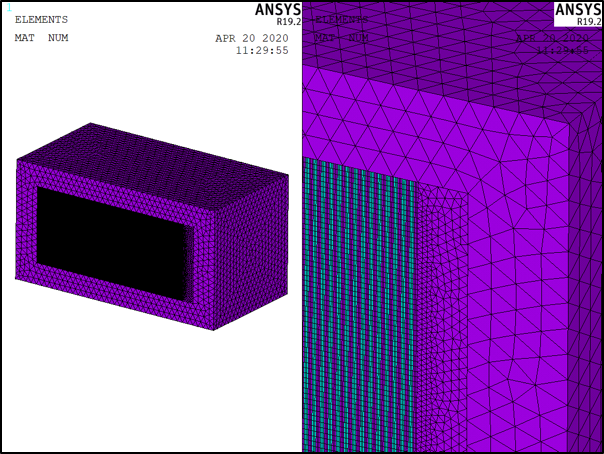
\includegraphics[width=0.49\textwidth]{graphics/tms/Detector/tms_anl_Bmodel2.pdf}
\end{dunefigure}

\begin{dunefigure}[ANSYS model used for the magnetic field simulation.]{fig:tms_anl_Bfield1}
{Results of the magnetic field simulation.   Left:  Magnetic flux density (T), \SI{40}{\mm} plates in front.  Right:  Magnetic flux density beyond last \SI{40}{\mm}  plate. }
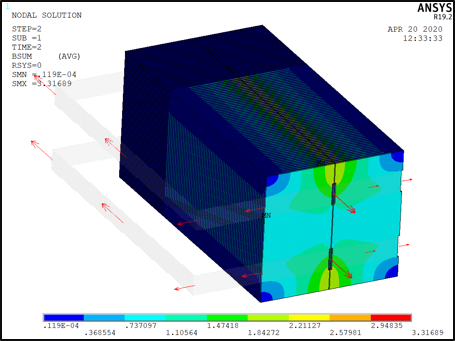
\includegraphics[width=0.49\textwidth]{graphics/tms/Detector/tms_anl_Bfield1.pdf} 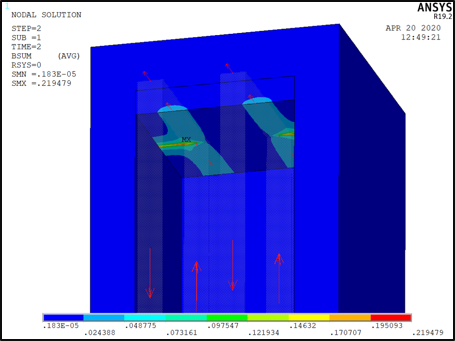
\includegraphics[width=0.49\textwidth]{graphics/tms/Detector/tms_anl_Bfield2.pdf}
\end{dunefigure}

%%%%%%%%%%%%%%%  One for each WBS element
\subsection{Detector Modules}
\label{sec:tms-des-panels}

The \dword{tms} will have \num{400} modules, each consisting of a single layer of plastic scintillator glued between \num{2} sheets of aluminum.  Each module will include \num{48} \SI{3.5}{\cm} wide $\times$ \SI{1}{\cm} thick $\times$ \SI{300}{\cm} long scintillators.  Each scintillator is outfitted with a single WLS fiber threaded through a hole centered in the scintillator and extending the full length.  

The \dword{wls} fibers exiting the scintillators will be divided into three groups of \num{16} and routed in a fiber tray to three separate fiber guide bars (FGB).  The ends of \dword{wls} fibers are precisely located by the FGB.  A manifold housing a 4x4 array of \dword{sipm} and a counter motherboard can then be mounted to each of the three FGBs for readout.  The module manifold is shown in Figure \ref{fig:tms_anl_module}.  

\begin{dunefigure}[Module Manifold Layout]{fig:tms_anl_module}
{Module manifold layout.}
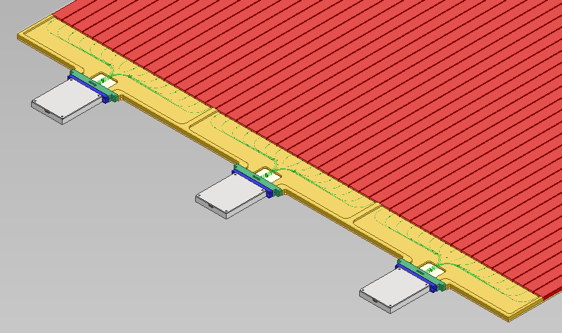
\includegraphics[width=0.6\textwidth]{graphics/tms/Detector/tms_anl_module.pdf}
\end{dunefigure}

%%%%%%%%%%%%%%%  One for each WBS element
\subsection{Detector Electronics}
\label{sec:tms-des-electronics}
\subsubsection{On-Panel Boards}
\label{sec:tms-des-elect-OPB}


The wavelength-shifting fibers are attached to the
16-channel \dword{sipm} (Hamamatsu S13361-2050AE-04) via a 
custom connector (possibly \threed printed with an included light difuser). This is mounted on one of the two electronics subsystems, the On-Panel Board (OPB).

From the \dword{sipm}, the signals are amplified by an 8$\times$ preamp,
and from there to the Analog Front-End/\dshort{adc} chip. We
have tentatively selected the eight-channel Texas Instrument AFE5807 \cite{AFE5807}.
This chip digitizes at 80\,MSPS and outputs \dword{lvds}.

Thee \dword{lvds} signals are sent via 50 pair/100 conductor cable
to the data concentrators.
 
\subsubsection{Data Concentrators}
\label{sec:tms-des-elect-DC}

There are eight data concentrators, each servicing fifty
panels or 2400 channels. Their job is to mate the
 \dword{lvds}  signals from the OPBs to the \dword{daq}. Each contains
a \dword{fpga} to do the fast processing and a small single-board
computer (SBC) to send this data over Ethernet as 
TCP/IP packets or \dword{udp} datagrams. Each packet will
contain the channel number, the event time, and the channel
energy. The DAQ does not require that the packets be in  chronological order.

%%%%%%%%%%%%%%%  One for each WBS element
\subsection{Transport and Installation}
\label{sec:tms-des-transport}

Installation of the detector components will be done by the Installation and Integration group, with some assistance for the first few panels by the construction team. The detector begins construction from the downstream side. A strongback is mounted to the support structure at a slight angle, and then Panel Layer 100 is attached. Steel and scintillator panels are then attached in alternating layers.

Because we envision three production sites, we have budgeted to move the panels from these sites to Fermilab. We intend to keep one extra day's worth of panels at the Near Detector Hall, so that we can take advantage of work going faster than planned.

%%%%%%%%%%%%%%%%%%%%%%%%%%%%%%%%

\section{Interfaces}
\label{sec:tms-interface}

Table~\ref{tbl:larndinterfaces} contains a summary and brief description of all the interfaces between the \dword{tms} consortium and other consortia, working groups, and task forces, with references to the current version of the interface documents describing those interfaces.  
Drawings of the mechanical interfaces and diagrams of the electrical interfaces are 
included in the interface documents as appropriate.
It is expected that further refinements of the interface documents will take place prior to the final \dword{prr} for the detector. The interface documents specify the responsibility of different consortia or groups during all phases of the experiment including design and prototyping, integration,  installation, and  commissioning.


\begin{dunetable}
[\dshort{tms} interface links]
{p{0.25\textwidth}p{0.5\textwidth}l}
{tbl:larndinterfaces}
{\dshort{tms} interface links}
Interfacing System & Description & Linked Reference \\ \toprowrule
Cryostat      &  (desc)
& %\citedocdb{?} 
\\ \colhline

\dshort{duneprism} &  (desc)
& %\citedocdb{?}
\\ \colhline

\dshort{sand}  &  (desc)
& %\citedocdb{?}
\\ \colhline

Computing  &  (desc)
& %\citedocdb{?}
\\ \colhline

\dshort{daq}    &  (desc)
& %\citedocdb{?}
\\
\end{dunetable}



%%%%%%%%%%%%%%%%%%%%%%%%%%%%%%%%
\section{Risks, Hazards and Their Mitigations}
\label{sec:tms-risks-hazards}


\section{Risks and Mitigations}
\label{sec:tms-risks}

%Table~\ref{tab:risks:ND-LAr} contains a list of all the
% HAT: replaced first sentence
Table~\ref{tab:table-tms-risks} contains a list of all the
risks that \dword{dune} is currently holding in the \dword{tms} risk register.  Each line includes the official \dword{dune} risk register identification number, a description of the risk, the proposed mitigation for the risk, and finally three columns rating the post-mitigation (P)robability that the risk described comes to pass, the degree of (C)ost risk for that line, and the degree of (S)chedule risk.  Risk levels are defined as (L)ow (<10\% probability of occurring, <5\% cost impact, <2 month schedule impact), (M)edium (10 to 25\% probability of occurring, 5\% to 20\% cost impact, 2 to 6 month schedule impact), or (H)igh (>25\% probability of occurring, >20\% cost impact, >6 month schedule impact).  Most of these risks are reduced to a ``Low'' level following mitigation (as shown in the table), although several of them currently hold a higher risk levels (pre-mitigation), due to the early stage of development of the \dword{tms} system relative to other systems.  

In the following sections, we present a narrative description of each of the risks and the proposed mitigation.

\fixme{Anne needs to get risk table template put together}
%\begin{dunetable}
%[Placeholder for risks table]
%{cc}
%{tab:table-tms-risks}
%{Placeholder for Risks Table - it will be generated from a spreadsheet}
%Rows & Counts \\ \toprowrule
%Row 1 & First \\ \colhline
%Row 2 & Second \\ \colhline
%Row 3 & Third \\ % no \colhline on final row
%\end{dunetable}
%\input{generated/risks-longtable-ND-LAr.tex}


Risks contained in the DUNE risk register are shown in Table~\ref{tab:table-tms-risks}. Steel and copper prices, like those of many commodities, tend to fluctuate. Getting the lowest possible price and starting construction as late as possible may be inconsistent goals, so our ability is limited to mitigate the risk by early purchase at a favorable price.  The \dword{sipm} prices have been falling since their introduction; this trend may continue.

\begin{dunetable}
[\dword{tms} Risks]
{ccc}
{tab:table-tms-risks}
{\dword{tms} Risks from Risk Register}
Risk Number & Category & Risk \\ \toprowrule
RT-131-ND-068 & Uncertainty & Copper Cost Fluctuations \\ \colhline
RT-131-ND-070 & Uncertainty & Steel Cost Fluctuations \\ \colhline
RT-131-ND-072 & Risk & Cable Noise Issues \\ \colhline
RT-131-ND-074 & Opportunity & SiPM Cost Fluctuations \\ 
\end{dunetable}

The only technical risk in the register is the potential for cable noise pickup, most likely from the magnet coils. To reduce this risk, this will be prototyped, verifying that LVDS cables can successfully operate near high-current and potentially noisy coils. More details on this prototyping plan can be found in that section.

There are some less significant risks, mostly opportunities, that have not risen to the level of the DUNE-wide risk register. Many of these are described in the Prototyping section, as successful prototyping will enable these opportunities to be realized.

In addition to typical construction hazards (e.g. hand tools), there are two specific to this. One is the use of glues and epoxies, which are hazardous materials. The other is the weight of the panels, approximately 200 pounds. This is heavy enough to potentially cause injury, but light enough for inexperienced workers to be tempted to move and position it without following procedure and using the proper fixturing. Written procedures for each step of module production will be established, and a strong safety culture is a requirement for site selection.

While not strictly a risk, the panels are ``trapped'' by the coils; coil removal is a requirement for module replacement. The acceptance loss and additional costs were considered too much given the potential benefits of repairing one or two counters that have gone bad.

%%%%%%%%%%%%%%%%%%%%%%%%%%%%%%%%
\section{Production Plans and Schedule}
\label{sec:tms-org-sched}

\subsection{Steel Procurement}

The steel plates will be produced in industry, cut to shape. The remaining dimension is in $z$, and we have requirements on both flatness and thickness. The flatness specification is 0.3\% or less within the central 3.2~m (in $y$) and 0.6\% or less outside that.

We doi not have a hard thickness specification, although we would like to keep the systematic uncertainty on energy scale to within a budget of 1\%, we need to know the material the muon traverses to within that same 1\%. The 0.3\% flatness specification implies a 0.6\% tolerance on thickness, so the only remaining uncertainty would be due to density/composition variation in the plates.

Plates will be surveyed on both sides, and the two sides registered with respect to each other so that thickness can be inferred from what are fundamentally measurements of flatness. Care will be taken to ensure that the plates are not bent during this procedure by keeping any applied bending moment to a minimum. Additionally, the plates will be individually weighed.

\subsection{Module Production}
The basic fabrication steps to fabricate a module are as follows:

Step 1. Cut Scintillators to Length (as shown in Figure~\ref{fig:tms_panel_phase_1}).
\begin{itemize}
\item{Scintillators are inspected visually and dimensionally.}
\item{A number of scintillators - for example, 12 - are loaded into a custom cut off rack.}
\item{Scintillators are cut to the same length with a cut off saw.}
\item{The fiber holes are then chamfered at each end using a center point drill.}
\end{itemize}

\begin{dunefigure}[Cutting scintillator to length]{fig:tms_panel_phase_1}
{Cutting Scintillator to length and prepping fiber holes (courtesy of Mu2e)}
\begin{center}
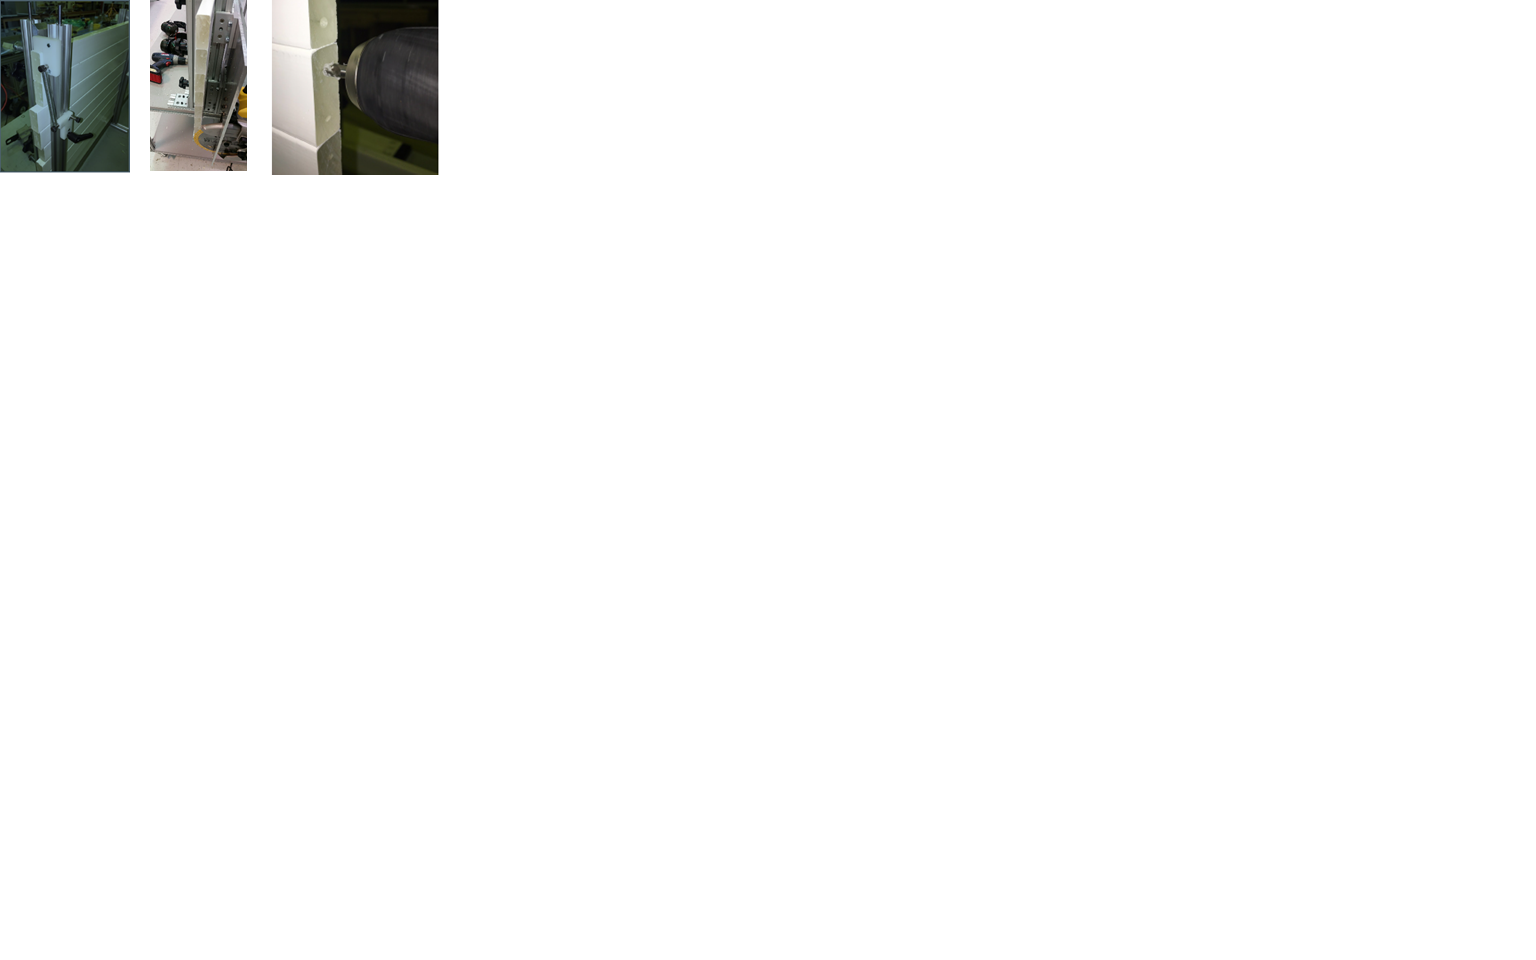
\includegraphics[trim= 0 580 0 0 clip, width=3.5\textwidth]{graphics/tms/TMS-Other/Fig39.png}
\end{center}
\end{dunefigure}

Step 2.	Assemble Scintillators, Fiber Tray, Wedge Plate and bottom Cover Plate.
\begin{itemize}
\item{Bottom cover plates are placed on a custom assembly table.}
\item{A dry run is conducted to optimize the placement of each scintillator and to make a plan for any shimming that must be done.}
\item{Orientation and location is noted and  then the scintillators are removed.}
\item{Epoxy is spread on the on plate, as shown in Figure~\ref{fig:tms_panel_phase_2a}.} 
\item{The fiber tray, wedge plate and scintillators are placed in glue.} 
\item{The assembly is bagged and placed under vacuum while epoxy sets as shown in Figure~\ref{fig:tms_panel_phase_2b}.} 
\end{itemize}

\begin{dunefigure}[Applying epoxy to bottom plate]{fig:tms_panel_phase_2a}
{Applying epoxy to bottom plate.}
\begin{center}
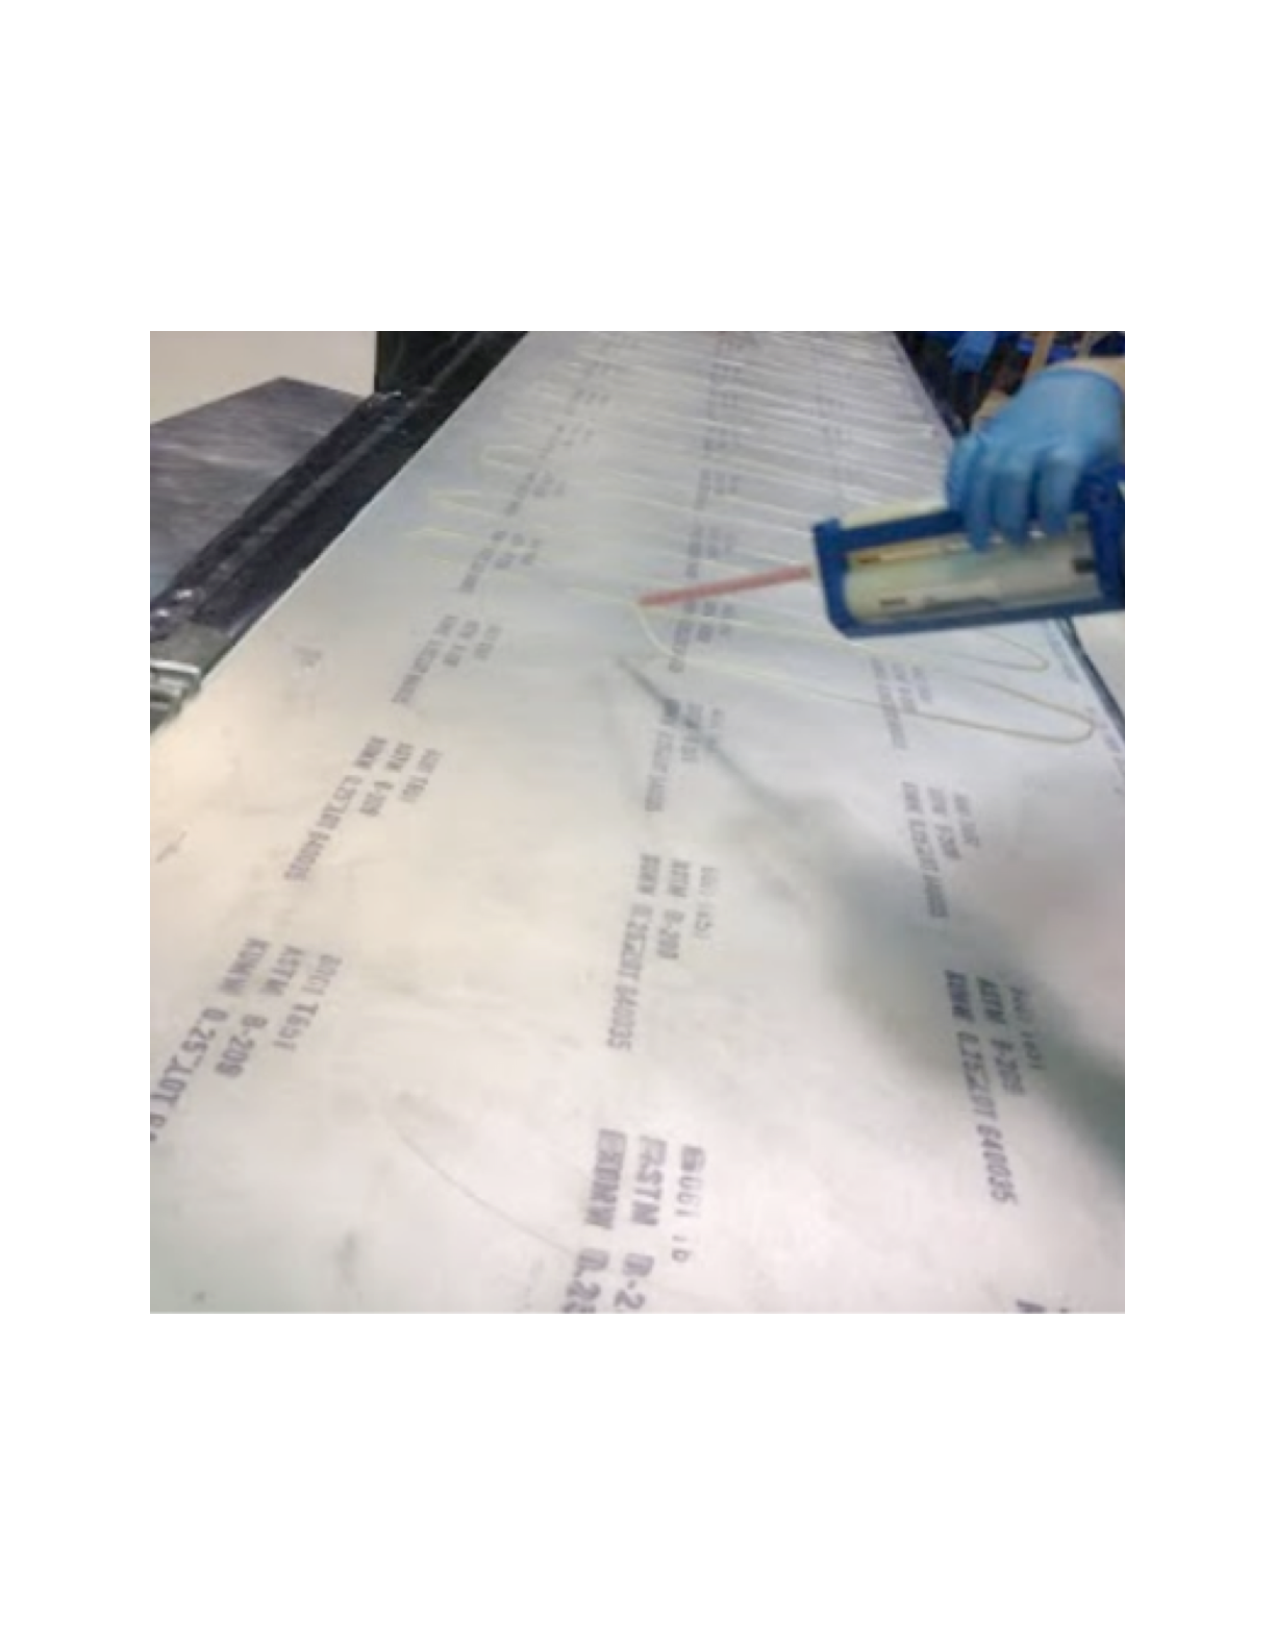
\includegraphics[width=0.5\textwidth]{graphics/tms/TMS-Other/tms_anl_fig37.pdf}
\end{center}
\end{dunefigure}

\begin{dunefigure}[Bagging assembly]{fig:tms_panel_phase_2b}
{Bagging assembly and putting it under vacuum while the epoxy sets}
\begin{center}
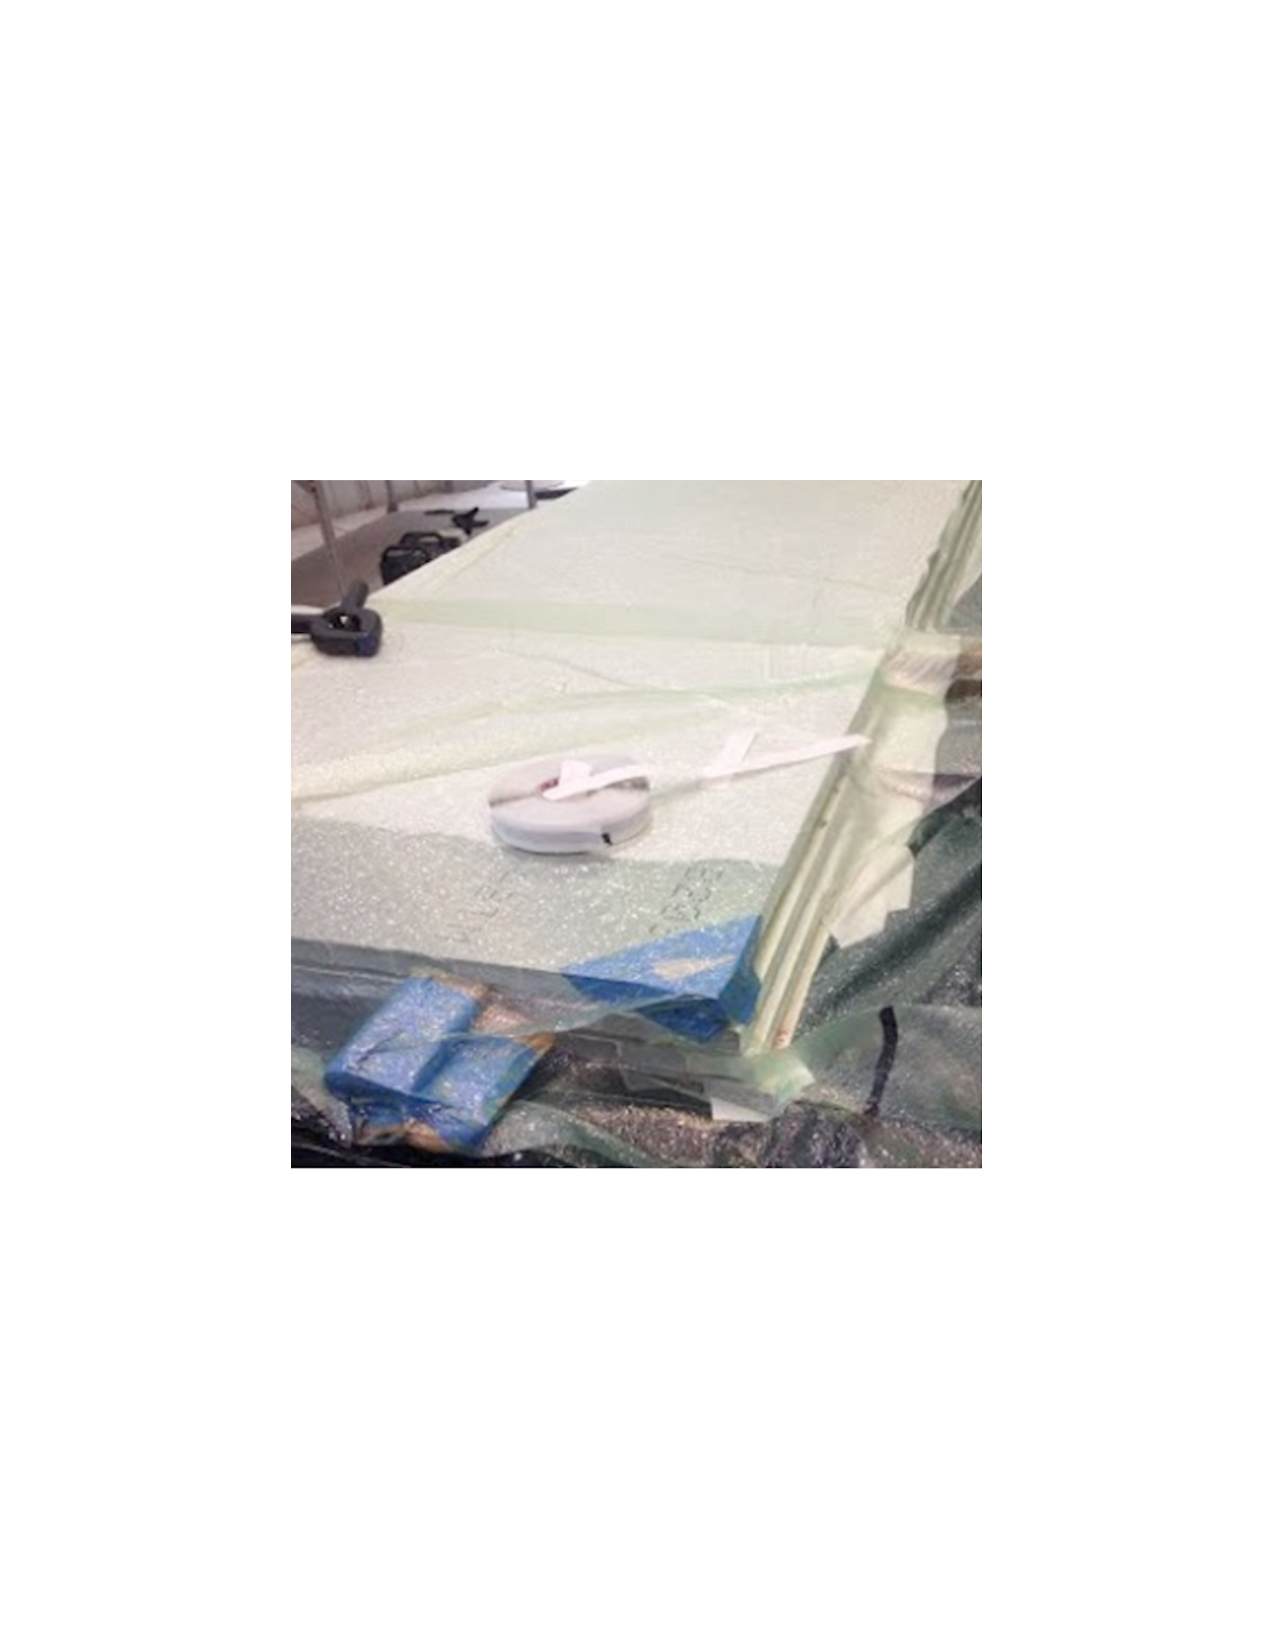
\includegraphics[width=0.5\textwidth]{graphics/tms/TMS-Other/tms_anl_fig41.pdf}
\end{center}
\end{dunefigure}
 
Step 3.	Fibers Installed and Routed to Fiber Guide Bars. %see Figure 43
\begin{itemize}
\item{Fibers are removed from the spool mounted to a fiber spool cart and are cut to length based on the scintillator position.}
\item{Fiber guide bars are installed on the fiber tray.}
\item{Epoxy is applied to each fiber as they are threaded through the hole in each scintillator, the method used for the similar length scintillator bars of the \dword{minerva} detector.  The fiber exits the scintillator and is routed in the fiber tray to the appropriate hole in one of the (3) fiber guide bars.}
\item{The fibers are potted in position at the fiber guide bars as shown in Figure~\ref{fig:tms_panel_phase_3a}}
\end{itemize}

\begin{dunefigure}[Fiber routing and fiber guide bars]{fig:tms_panel_phase_3a}
{Fiber routing and fiber guide bars}
\includegraphics[trim= 0 500 0 0 clip, width=2.7\textwidth]{graphics/tms/TMS-Other/phase3a.png}
\end{dunefigure}

Step 4.	Intermediate Quality Control Tests:
\begin{itemize}
\item{Before final assembly of a module, there are several QC checks that could be performed: fiber transmission test, fiber imaging, and possibly a source test.}
\item{A fiber transmission test could be performed using LED blocks mounted to the wedge end
%(Figure 44) 
and LED or Photo Diode blocks mounted to the fiber guide bars.}
\end{itemize}

Step 5.	Final Assembly of Module:% see Figure 45
\begin{itemize}
\item{Epoxy is spread on the scintillators, fiber tray, and wedge plate as shown in Figure~\ref{fig:tms_panel_phase_5a}.}
\item{The top cover plate is installed.}
\item{The assembly is bagged and placed under vacuum  while the epoxy sets.}
\end{itemize}
  
\begin{dunefigure}[Top cover gluing]{fig:tms_panel_phase_5a}
{Top cover gluing}
\includegraphics[trim= 0 600 0 0 clip, width=3.1\textwidth]{graphics/tms/TMS-Other/phase5a.png}
\end{dunefigure}


Step 6.	Flycut to Polish the Fiber Ends.
\begin{itemize}
\item{A hot knife is used to cut the fibers flush with the fiber guide bars.}
\item{The face of the fiber guide bar is flycut as shown in Figure~\ref{fig:tms_panel_phase_5b}.}
\item{A protective cover block is then installed.}
\end{itemize}

\begin{dunefigure}[Flycutting fibers]{fig:tms_panel_phase_5b}
{Flycutting fibers at fiber guide bars}
\includegraphics[trim= 0 600 0 0 clip, width=3.1\textwidth]{graphics/tms/TMS-Other/phase5b.png}
\end{dunefigure}

Step 7. Final Light Tightening Measures:
\begin{itemize}
\item{Edges are taped.}
\end{itemize}

Step 8.	Final Quality Control Tests:
\begin{itemize}
\item{Measurements are made on each module to ensure that it meets dimensional tolerances. }
\item{Tthe response of each module to minimum ionizing particles should be studied using a cosmic ray test stand. This may occur at the Fermilab receiving site in addition to or instead of the production site.}
\end{itemize}

Both a bottom-up estimate of construction time from the above tasks plus a top-down scaling from MINOS imply a total construction rate of 2 to 2.5 panels per week. Figure~\ref{fig:tms_panel_gantt} shows a consolidated production plan for one site. We envision two teams per site: Team One executes Tasks 2 and 3 above, and Team Two executes everything else.

\begin{dunefigure}[TMS Panel Gantt]{fig:tms_panel_gantt}
{Timeline for panel construction. For simplicity, glue curing time is not included. Colors indicate individual panels. Lighter colors represent Team One activities and darker colors represent Team Two.}
\includegraphics[trim= 0 300 0 0,  clip,width=1.00\textwidth]{graphics/tms/TMS-Other/TMSPanelGantt.pdf} 
\end{dunefigure}

The time to complete a single module is just under one week, plus two days of glue curing time. As stated before, the maximum site rate is 2-2.5 panels per week. With two sites, it will take approximately 22 months to construct all of the panels. We hope to be able to set up three sites to build in some contingency, as well as reducing the risk of one site having to slow or stop production.

The 22 months needed to assemble the panels drives the overall schedule, shown in Table \ref{tab:table-tms-schedule}. This shows we need to set the go/no-go decision date 34 months before the first beam is delivered. It assumes a six month period to go out for bid, issue the Purchase Orders and delivery of parts, particularly long lead items like wavelength-shifting fiber. It includes a 20\% contingency on the time of construction. While some schedule risk is mitigated by having a third panel construction site, some of the risk is correlated: a delay in delivery of parts affects all sites.

There is one month scheduled to wind the magnet. While most of the infrastructure and magnet will be constructed in parallel with the panels, the coils can be wound only after the panels are installed.

\begin{dunetable}[\dshort{tms} High Level Schedule]
{cc}
{tab:table-tms-schedule}
{\dshort{tms} High Level Schedule.} 
Activity & Duration\\ \toprowrule
POs issued and delivery of parts & 6 months\\ \colhline
Panel Construction               & 22 months\\ \colhline
Coil Winding                     & 1 month \\ \colhline
Contingency                      & 5 months\\ \colhline
\rowcolor{dunepeach}Total        & 34 months \\ 
\end{dunetable}


\label{sec:tms-construc}



 
%%%%%%%%%%%%%%%%%%%%%%%%%%%%%%%%
\section{Prototyping and Other Studies}
\label{sec:tms-proto}

\subsection{Construction Time and Motion Studies}

The construction time estimates shown in this document were derived from \dword{minos} and \dword{mu2e} experience with similar counters, using both a top-down and bottom-up methodology (which agree to better than 10\%.) Nevertheless, we would very much like to reduce the uncertainty on the construction time, as this directly contributes to the last possible go/no-go date for building the \dword{tms}.

We had planned to build some mechanical-only prototypes, using clear fiber and ordinary polystyrene in place of scintillator. However, the titanium dioxide co-extruded surface of the scintillator causes it to handle very differently than plain polystyrene. We are now switching to non-science-grade scintillator for these mechanical studies.

\subsection{Magnet Value Engineering}
There are three ways to increase the magnetic field. One can increase current, increasing the power needed and the heat that needs to be removed. Both of these add costs. Alternatively, one can increase the number of turns, which increases the copper costs as well as the power supply costs, but to a lesser degree than above. Finally, one can increase the amount of steel above and below the coils and panels. This increases the steel cost, as well as causing issues related to the flatness specification, the assembly time, and the mass that needs to be moved by \dword{duneprism}.

The present design has been optimized the various trade-offs based on 2020 prices. The situation may be different immediately before construction, so at that time we will hold a round of value engineering to see if a different combination of iron, steel and power provides the same performance at lower cost.

In particular, the decision to air-cool should be revisited. The present design has the individual coils air-cooled and only loosely thermally coupled to the steel. An alternative would be closed loop water cooling, where the cables are cooled by water and that heat transferred to the steel, where it is coupled to the air and cooled with the rest of the hall. Presently, this is more expensive: the additional cost of the power supplies and chillers exceeds the savings from the copper. This situation may not be the case in a few years.

\subsection{Signal Cables and Noise}
A high level risk (DUNE RT-131-ND-072) is the issue of unacceptable noise pickup on the cables from the On-Panel Boards to the Data Concentrators. These by necessity run near the magnet coils. Since the coils are 30,000 ampere-turns, a 0.1\% RMS noise level is the equivalent of 30~amperes. A series of prototyping and testing has been initiated at Wichita State to set a crosstalk/sensitivity specification and ensure we can purchase cables that meet that specification.  Alternative designs will be explored if needed, such as using external shielding / shielded conduit, or switching to optical connections, both of which have negative cost and schedule implications.

\subsection{Steel Plate Thickness}

The design of forty ``thin'' (15~mm) and sixty ``thick'' (40~mm) plates appears to meet our performance goals. One could imagine improving the performance beyond our initial goals by using three thicknesses of steel plates rather than two: an intermediate thickness between the thin and thick plates.

While this will improve performance, it does so primarily in the 2-3~GeV range, where we already do well. The place where this detector struggles the most is at very low momentum, where there are only a few hits before the muon ranges out. This could be addressed by using thinner (perhaps 10~mm, perhaps even less) plates in the very first few layers. Such plates present their own challenges, including procuring them and ensuring they can withstand the megnetic and mechanical forces.

\subsection{Fiber Location Within Scintillator}

The MINOS design had the wavelength shifting fiber on the face of the scintillator strip. \dword{mu2e} took a different approach, co-extruding a thin tube through the center of each scintillator. All other things being equal, the \dword{mu2e} solution will produce more light, but construction aspects may reduce or eliminate this potential benefit. Specifically, it is easier to get a good optical connection when gluing fibers in if one has access to the groove. 

In the center-fiber design, one inserts the fiber into the center column and then fills that column with low viscosity glue. This requires the counter to be ideally vertical but at least inclined so that bubbles in the glue rise. The effectiveness of this as well as the schedule implications remain to be demonstrated. A glue-less design is a similar option to be considered.

\subsection{Assembly and Module Strength}

The design described above is very glue-intensive. Glue provides the strength of the modules. An alternative is to make the aluminum frame and covers - informally the ``box'' - structural in addition to simply being light-tight. This would require strengthening the boxes with aluminum ribs and/or aluminum Hexcel\texttrademark{}.

This reduces the amount of glue required, and glue is a hazardous material. It also opens up the possibility for repairing a panel mid-assembly in situations where gluing would preclude that. It may shorten the overall production time. It also eliminates the whole-panel cure time. This has only a minor impact on production rate, but it eliminates the need for a separate curing station and any motion of the panels to and from these stations.

\subsection{Fiber attachment to SiPM}

One of the most time consuming aspects of the construction is attaching the sixteen fibers to a single SiPM. At this stage of the construction process, the fibers have been glued in place at the other end, and have just completed a small radius bend. This is compounded by Hamamatsu's recommendation not to use optical grease, which runs counter to past experience. 

Strain relief of the fibers, such as by routing them through a styrofoam channel, will make construction easier. We are also investigating a 3D-printed optical coupler to mate the fibers to the SiPM. This would save a great deal of production time, perhaps shortening Team One's activities enough so that they can take on one of Team Two's responsibilities. That would allow for significantly faster production and potentially a later go/no-go decision date.

However this attachment is made, we need a better handle on the behavior of the SiPM. Open questions include: is there any benefit to a diffuser, no matter how one is constructed? Is the cross-talk significant? Do we need to map the fibers to avoid adjacent channel cross-talk? Is a coupling without optical grease really the correct solution?


%%%%%%%%%%%%%%%%%%%%%%%%%%%%%%%%%%%%%%%%%%%%%%%%%%%%%%%%%%%%%%%% 
\begin{comment} % comment here to end
\fixme{The following sections are not in the new structure; I'm keeping them at the end here for now, in case you want to include one or more of them later.}

%%%%%%%%%%%%%%%%%%%%%%%%%%%%%%%% Not in Tim's new organization
\section{Safety Concerns}
\label{sec:tms-safety}


%%%%%%%%%%%%%%%%%%%%%%%%%%%%%%%% Not in Tim's new organization
\section{Calibration}
\label{sec:tms-calib}

%%%%%%%%%%%%%%%%%%%%%%%%%%%%%%%% Not in Tim's new organization
\section{Quality Assurance}
\label{sec:tms-qa}

%%%%%%%%%%%%%%%%%%%%%%%%%%%%%%%% Not in Tim's new organization
\section{Production, Assembly, and Quality Control}
\label{sec:tms-qc}

%%%%%%%%%%%%%%%%%%%%%%%%%%%%%%%% Not in Tim's new organization
\section{Transport and Handling}
\label{sec:tms-transport}

%%%%%%%%%%%%%%%%%%%%%%%%%%%%%%%% Not in Tim's new organization
\section{Installation, Integration, and Commissioning}
\label{sec:tms-iic}

%%%%%%%%%%%%%%%%%%%%%%%%%%%%%%%% Not in Tim's new organization
\section{Organization}
\label{sec:tms-org}

%%%%%%%%%%%%%%% Not in Tim's new organization
\subsection{Participating Institutions}
\label{sec:fdsp-org-inst}
%\metainfo{\color{red}\bf  Content: Segreto/Warner}

The \dword{tms} consortium benefits from the contributions of many institutions and facilities in \fixme{several countries? or the U.S. and ??}.  Table~\ref{tab:tms-institutes}
lists the member institutions. 

\begin{longtable}
{ll}
\caption{\dshort{tms} consortium institutions}\\ \colhline
\rowcolor{dunetablecolor} Member Institute  &  Country       \\  \toprowrule
univ 1 &  \\ \colhline
univ 2 &  \\ \colhline
univ 3 &  \\ 
\label{tab:tms-institutes}
\end{longtable}


\end{comment}









